% DEEP folds: WHIR soundness from list size alone.
%
%   build:  mkdir -p .build && pdflatex -interaction=nonstopmode -halt-on-error -output-directory=.build main.tex
%           (then, for the bibliography: cd .build && BIBINPUTS=..: bibtex main, and pdflatex twice more)
\documentclass[11pt]{article}
% Packages, notation and theorem environments.
% Notation follows Annex B of the leanVM specification (doc/leanvm/preamble/macros.tex).
\usepackage[T1]{fontenc}
\usepackage[utf8]{inputenc}
\usepackage{lmodern}
\usepackage[margin=1in]{geometry}
\usepackage{microtype}
\usepackage{amsmath,amssymb,amsthm,mathtools}
\usepackage{tabularx,booktabs,longtable,array}
\usepackage{enumitem}
\usepackage{xcolor}
\usepackage{tikz}
\usetikzlibrary{arrows.meta}
\usepackage{listings}
\usepackage[colorlinks=true,linkcolor=blue!50!black,citecolor=blue!50!black,urlcolor=blue!50!black]{hyperref}

\emergencystretch=1.5em

% ragged-right table cells: narrow justified columns set badly
\newcolumntype{L}[1]{>{\raggedright\arraybackslash}p{#1}}
\newcolumntype{Y}{>{\raggedright\arraybackslash}X}

% fields, multilinears
\newcommand{\F}{\mathbb{F}}
\newcommand{\Ftwo}{\mathbb{F}_2}
\newcommand{\K}{K}
\newcommand{\E}{E}
\newcommand{\q}{q}
\newcommand{\mle}[1]{\widetilde{#1}}
\newcommand{\eq}{\operatorname{eq}}
\newcommand{\cube}[1]{\{0,1\}^{#1}}
\newcommand{\inner}[2]{\langle #1,\, #2 \rangle}
\newcommand{\fc}{\chi}
\newcommand{\qeq}{\stackrel{?}{=}}

% codes and the PCS, as in Annex B
\newcommand{\Enc}{\mathrm{Enc}}
\newcommand{\RS}{\mathrm{RS}}
\newcommand{\nv}{M}
\newcommand{\nlev}{\Lambda}
\newcommand{\rate}{\rho}
\newcommand{\rexp}{\nu}
\newcommand{\rc}[1]{c^{(#1)}}
\newcommand{\nq}{\omega}
\newcommand{\blen}{n}
\newcommand{\dom}{\mathcal{D}}
\newcommand{\orc}{Z}
\newcommand{\lst}{\mathcal{L}}
\newcommand{\aset}{\mathcal{A}}
\newcommand{\agr}{t}
\newcommand{\dgr}{\mathsf{d}}
\newcommand{\jl}{\mathsf{L}}
\newcommand{\afa}{\mathsf{a}}
\newcommand{\afb}{\mathsf{b}}
\newcommand{\tabx}[1]{v_{X,#1}}
\newcommand{\phigh}{\mathbf{h}}
\newcommand{\epsaff}{\varepsilon_{\mathrm{aff}}}
\newcommand{\vansub}{\mathcal{V}}
\newcommand{\Wn}[1]{\widehat{\vansub}_{#1}}
\newcommand{\novel}{\mathcal{X}}
\newcommand{\mpoly}{\mathcal{P}}

% this paper
\newcommand{\ev}{\operatorname{ev}}            % the point evaluation functional
\newcommand{\cand}{\mathcal{T}}                % the set of candidates (challenge, list member of the fold)
\newcommand{\cls}{\mathcal{C}}                 % a class of candidates
\newcommand{\Exc}{\operatorname{Exc}}          % the exceptional set of point tuples
\newcommand{\pot}{\Psi}                        % the potential of a level
\newcommand{\thr}{\Theta}                      % the triple threshold K_0 (K_0 - 1)(K_0 - M)
\newcommand{\Kz}{K_0}                          % an integer constant of the analysis
\newcommand{\dsc}{\tau}                        % the discount of the potential
\newcommand{\epp}{\epsilon}                    % the error of one point
\newcommand{\Lb}{\mathrm{ListBound}}
\newcommand{\HK}{\mathrm{H}_{\K}}
\newcommand{\HE}{\mathrm{H}_{\E}}
\newcommand{\pull}{\operatorname{pull}}
\newcommand{\Bad}{\mathrm{Bad}}
\newcommand{\treeN}{\mathsf{N}}
\newcommand{\loc}{L}                           % a subspace polynomial L_V
\newcommand{\Zs}{Z}                            % a locator Z_S (context separates it from the oracle)
\newcommand{\Prob}{\Pr}
\newcommand{\Ex}{\mathbb{E}}
\newcommand{\bP}{\mathbf{P}}
\newcommand{\bV}{\mathbf{V}}
\DeclareMathOperator{\agrset}{agr}

% Lean names and status labels
\DeclareUrlCommand\leanurl{\urlstyle{tt}}
\newcommand{\lean}[1]{\leanurl{#1}}
\newcommand{\leanfile}[1]{\leanurl{lean/#1}}
\newcommand{\leansub}[2]{\leanurl{#1}\textsubscript{\texttt{#2}}}
\newcommand{\stmc}{\textsc{machine-checked}}
\newcommand{\stpr}{\textsc{proved}}
\newcommand{\stcj}{\textsc{conjectured}}
\newcommand{\status}[1]{\par\smallskip\noindent{\small\sloppy\textbf{Status.} #1\par}\smallskip}

% theorem environments
\theoremstyle{plain}
\newtheorem{theorem}{Theorem}[section]
\newtheorem{lemma}[theorem]{Lemma}
\newtheorem{corollary}[theorem]{Corollary}
\newtheorem{proposition}[theorem]{Proposition}
\newtheorem{conjecture}[theorem]{Conjecture}
\newtheorem{hypothesis}[theorem]{Hypothesis}
\theoremstyle{definition}
\newtheorem{definition}[theorem]{Definition}
\newtheorem{protocol}[theorem]{Protocol}
\newtheorem{problem}[theorem]{Open problem}
\theoremstyle{remark}
\newtheorem*{remark}{Remark}

% Lean listings
\lstdefinelanguage{lean}{
  morekeywords={theorem,lemma,def,noncomputable,by,fun,if,then,else,let,have,show,from,open,variable,abbrev},
  sensitive=true,
  morecomment=[l]{--},
}
\lstset{
  language=lean,
  basicstyle=\ttfamily\footnotesize,
  keywordstyle=\bfseries,
  columns=fullflexible,
  keepspaces=true,
  breaklines=true,
  breakindent=2em,
  frame=single,
  framesep=4pt,
  xleftmargin=6pt,
  xrightmargin=6pt,
  extendedchars=true,
  literate=
    {ℕ}{{$\mathbb{N}$}}1 {ℚ}{{$\mathbb{Q}$}}1 {∞}{{$\infty$}}1
    {→}{{$\to$}}1 {↔}{{$\leftrightarrow$}}1 {∀}{{$\forall$}}1 {∃}{{$\exists$}}1
    {≤}{{$\le$}}1 {≥}{{$\ge$}}1 {≠}{{$\ne$}}1 {¬}{{$\neg$}}1 {∧}{{$\wedge$}}1 {∨}{{$\vee$}}1
    {∈}{{$\in$}}1 {∉}{{$\notin$}}1 {⊆}{{$\subseteq$}}1 {∑}{{$\sum$}}1 {∏}{{$\prod$}}1
    {⊕}{{$\oplus$}}1 {×}{{$\times$}}1 {ˢ}{{$^{s}$}}1 {•}{{$\bullet$}}1 {∘}{{$\circ$}}1
    {⁻}{{$^{-}$}}1 {¹}{{$^{1}$}}1
    {₀}{{$_0$}}1 {₁}{{$_1$}}1 {₂}{{$_2$}}1 {₃}{{$_3$}}1 {ₗ}{{$_{l}$}}1
    {α}{{$\alpha$}}1 {β}{{$\beta$}}1 {σ}{{$\sigma$}}1 {τ}{{$\tau$}}1 {ι}{{$\iota$}}1 {κ}{{$\kappa$}}1
    {ζ}{{$\zeta$}}1 {φ}{{$\varphi$}}1 {Λ}{{$\Lambda$}}1 {ℓ}{{$\ell$}}1 {λ}{{$\lambda$}}1 {θ}{{$\theta$}}1
    {Γ}{{$\Gamma$}}1 {𝒞}{{$\mathcal{C}$}}1 {𝒯}{{$\mathcal{T}$}}1 {ε}{{$\varepsilon$}}1 {π}{{$\pi$}}1 {Θ}{{$\Theta$}}1
    {⟨}{{$\langle$}}1 {⟩}{{$\rangle$}}1 {↑}{{$\uparrow$}}1 {⊢}{{$\vdash$}}1 {∣}{{$\mid$}}1
}


\title{\bf DEEP folds: WHIR soundness from list size alone}
\author{}
\date{}

\begin{document}
\maketitle

\begin{abstract}
The query counts of WHIR-like polynomial commitments are set by the agreement threshold at which each level is analysed, and the known analyses stop at the Johnson radius because they need mutual correlated agreement there. We study the variant used in leanVM (binary fields, subspace domains, affine folds). First we show how little room that protocol has below the Johnson radius, whatever the analysis: on every binary subspace domain there are explicit words with large lists of close codewords, correlated agreement fails wherever lists are large, and for that protocol a large list above the threshold is an attack. At rate $1/4$ this closes the gap between proof and attack; at the other rates it bounds how far any analysis of the same protocol could go. Then we modify the fold. After each commitment the verifier sends a few out-of-domain points, the prover answers with the committed polynomial's values there, and these claims are carried, unbatched, through the fold rounds. We prove that the modified protocol is round-by-round sound, and knowledge sound with a straight-line extractor that never list-decodes, with every verifier message at most $2^{-125}$ after its grind, under one hypothesis about the code: a bound on the number of codewords close to any word. No correlated agreement theorem is used, and the bound may be as large as $2^{100}$. At today's thresholds the hypothesis is the Johnson bound, so there the protocol is unconditionally sound, with essentially today's query counts: nothing is saved. Fewer queries need the hypothesis below the Johnson radius, and there it is open: no such bound is known for arbitrary words on any binary subspace domain. We state the problem, reduce it to single words over the small field (with a loss of at most a factor two in the ranges of interest), and collect what is proved, what is conjectured and why the known techniques fail. The fold-round lemma, the lemmas and per-message transitions of the soundness proof, the reductions of the hypothesis and the attack constructions (lower bounds on the lists, not their exact sizes) are machine-checked in Lean~4, and so is the composition of the transitions into a soundness theorem for an abstract model of the protocol, in which a committed word is a function as in the oracle model, the protocol is interactive with no grind, and each level has one batch of points. The link from that model to the concrete protocol (the encoder's identities, completeness, the Fiat-Shamir transformation with grinding, the Merkle commitments, the outer protocol, the extractor as an algorithm) is proved by hand or inherited, and the Lean development discharges the list hypothesis only in the unique-decoding range.
\end{abstract}

\tableofcontents
\newpage

\section{Introduction}\label{sec:intro}

\subsection{The question}

In a FRI-like polynomial commitment such as WHIR \cite{ACFY25}, the proof size and the verifier's work are dominated by the Merkle openings of the queries, and the number of queries of a level is set by one number, the \emph{agreement threshold} $\agr$ at which the level is analysed: a level of block length $\blen$ needs about $\lambda/\log_2(\blen/\agr)$ queries for $\lambda$ bits of security. For a Reed-Solomon code of rate $\rate$ the analyses that exist prove soundness for $\agr$ down to the Johnson radius $\sqrt\rate\,\blen$. Capacity, $\agr\approx\rate\,\blen$, would halve the query counts.

This paper is about the WHIR variant used in leanVM \cite{leanvm}: binary fields, an additive (subspace) evaluation domain, and the affine combiner of \cite{CWYZ26}. Its deployed query counts are already within a few queries of what the Johnson radius allows. We ask how far below the Johnson radius the thresholds can go, and what exactly would have to be proved.

For the protocol as it stands the answer is: nowhere at rate $1/4$ on subspace domains, and at the other rates no further than the agreement of the first large list (\S\ref{sec:gap}). The proof of soundness needs two things at the threshold, a small list of close codewords and \emph{mutual correlated agreement} (the fold of two words is close to a codeword only if the two words are close to a pair of codewords). On subspace domains both fail below the Johnson radius in places: there are explicit words with lists of $2^{26}$ to $2^{77}$ codewords, and wherever lists are large correlated agreement fails with them. Worse, for today's protocol a large list is an attack, not only a hole in the proof (\S\ref{sec:limit}).

\subsection{The idea}

We change the fold so that its soundness depends on the list size alone. Right after a commitment the verifier sends a few random points outside the domain, and the prover answers with the value of the committed polynomial at each of them (one field element per point, the lanes being combined with powers of a second random scalar). In every fold round, before the challenge, the prover says how each of these values splits over the two halves being folded; both parties then update the value for the folded polynomial. These \emph{point claims} are carried through the level next to the usual running claim and are never batched with it. That is the whole change (Protocol~\ref{prot:D}). We call it a DEEP fold, after the out-of-domain sampling of DEEP-FRI \cite{BGKS20}; STIR and WHIR \cite{ACFY24,ACFY25} already use out-of-domain samples to single out one member of a list at commitment time, and here the samples are in addition carried through the fold rounds.

Here is why it works. A fold challenge is a pair $(\afa,\afb)$, and the fold of a pair of polynomials $(F,G)$ is $G+(\afa+\afb X)F$.

\emph{First picture: a wrong list member keeps a line per point, and lines of different points have different slopes.} Suppose $(F,G)$ is close to the two halves of the committed word, but its values at a point $\zeta$ differ from the split $(y^F,y^G)$ the prover announced, by $(\delta^F,\delta^G)\ne(0,0)$. Its fold is consistent with the updated point claim exactly when
\[
\delta^G+(\afa+\afb\,\zeta)\,\delta^F=0 .
\]
This is a line in the plane of challenges. The prover chooses where the line lies, through its answers; its slope is set by $\zeta$, which the verifier chose. A second point $\zeta'\ne\zeta$ at which the pair also misses the answers gives a second line of a different slope, and two such lines meet in one challenge. So a list member that misses the answers at two points survives for at most one challenge out of $|\E|^2$, where in today's protocol it survives on a whole curve of about $|\E|$ challenges. (A member that misses the answers at one point only keeps a line; \S\ref{sec:sharp} says what that costs.) Large lists stop being dangerous.

\begin{figure}[t]
\centering
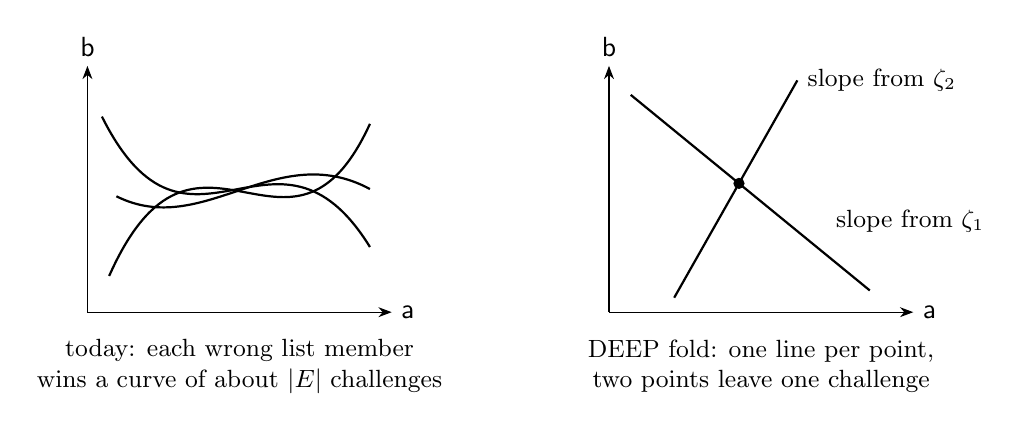
\begin{tikzpicture}[scale=0.92,>=Stealth]
\begin{scope}
\draw[->] (0,0) to (4.2,0) node[right] {$\afa$};
\draw[->] (0,0) to (0,3.4) node[above] {$\afb$};
\draw[thick] (0.3,0.5) .. controls (1.5,3.2) and (2.8,0.2) .. (3.9,2.6);
\draw[thick] (0.2,2.7) .. controls (1.4,0.3) and (2.6,3.0) .. (3.9,0.9);
\draw[thick] (0.4,1.6) .. controls (1.6,1.0) and (2.6,2.4) .. (3.9,1.7);
\node[align=center,font=\small] at (2.1,-0.75) {today: each wrong list member\\ wins a curve of about $|\E|$ challenges};
\end{scope}
\begin{scope}[xshift=7.2cm]
\draw[->] (0,0) to (4.2,0) node[right] {$\afa$};
\draw[->] (0,0) to (0,3.4) node[above] {$\afb$};
\draw[thick] (0.3,3.0) to (3.6,0.3);
\node[font=\small,anchor=west] at (3.0,1.25) {slope from $\zeta_1$};
\draw[thick] (0.9,0.2) to (2.6,3.2) node[right,font=\small] {slope from $\zeta_2$};
\fill (1.794,1.778) circle (2.2pt);
\node[align=center,font=\small] at (2.1,-0.75) {DEEP fold: one line per point,\\ two points leave one challenge};
\end{scope}
\end{tikzpicture}
\caption{The plane of fold challenges $(\afa,\afb)$ for one list member whose values disagree with the prover's answers.}\label{fig:lines}
\end{figure}

\emph{Second picture: three candidates consistent with one answer force a determinant to vanish.} The hard part of every fold analysis is the codewords close to the folded word that are \emph{not} folds of a close pair: ruling them out is what correlated agreement does, and below the Johnson radius it cannot be done. The point claims handle them without any such theorem. Take three polynomials $P_1,P_2,P_3$, close to the folded word at three different challenges $(\afa_k,\afb_k)$, all consistent with the same answers at a point: $P_k(\zeta)=y^G+(\afa_k+\afb_k\zeta)\,y^F$. Then the three rows $\bigl(P_k(\zeta),\,1,\,\afa_k+\afb_k\zeta\bigr)$ are orthogonal to the vector $(1,y^G,y^F)$, so
\[
\det\begin{pmatrix}P_1&1&\afa_1+\afb_1X\\P_2&1&\afa_2+\afb_2X\\P_3&1&\afa_3+\afb_3X\end{pmatrix}\ \text{vanishes at }X=\zeta .
\]
This determinant is a polynomial of degree at most one more than the code's; it depends on the three candidates and not on the answers; and it is the zero polynomial exactly when the three candidates are folds of one common pair. So three candidates that are \emph{not} folds of a common pair can all be consistent with one answer only if $\zeta$ is a root of a fixed nonzero polynomial, which a random $\zeta$ is with probability about $\text{degree}/|\E|\approx2^{-104}$, and $s$ independent points all are with probability $2^{-104s}$.

\emph{Counting.} There are at most $L$ close codewords per challenge, so at most $(L|\E|^2)^3$ triples. With enough points, only a negligible fraction of them survive, and then among any $\Kz$ challenges that the prover could win with one message, for $\Kz$ a few hundred times $|\E|$, more than $2|\E|$ are folds of a single pair $(F,G)$. That pair is a list member of the unfolded word and it matches the carried claims, so by the invariant it violates the running claim; but a pair with a false claim wins at most $2|\E|$ challenges. So fewer than $\Kz$ challenges can be won, and the fold round's error is $\Kz/|\E|^2$, a few hundred over $|\E|$, with no list factor and no correlated agreement term. The list size appears only in the number of points: at level $0$ each point is worth about $104$ bits, and $3\log_2L$ bits of the total pay for the list.

\subsection{Contributions and their status}\label{sec:contrib}

Every numbered theorem, lemma, proposition, corollary and conjecture below carries one of three labels. \stmc: the statement is a theorem of the accompanying Lean~4 development, with the Lean name and file given; where the Lean statement is more abstract or covers only part of the text, the label says so. \stpr: a complete proof by hand is given in this paper or, where explicitly said, in the cited source. No numbered statement carries this label on the strength of the project's working notes alone. Those notes are unpublished and do not accompany this paper. Some results quoted in the running text, in the tables of \S\ref{sec:proved} and in the status lines of the conjectures are proved only there: each such place says so, and their proofs are not reproduced here, so the reader cannot check them from this paper and should take them as claims of the project. A second reader within the project refereed part of the notes, and the text says which results were not refereed. This paper has had no external review. \stcj: not proved, with the evidence stated. Definitions and the protocol carry no label.

\begin{enumerate}[itemsep=2pt,topsep=3pt]
\item \emph{Today's protocol is at its limit} (\S\ref{sec:limit}). A path-cost model for attacks under Fiat-Shamir with grinding (\stpr). Large lists are attacks on the protocol of Annex~B (\stpr). Explicit lists on every binary subspace domain: at least $\blen-1$ codewords at agreement $\blen/2-1$ at rate $1/4$ (\stmc), which with the previous item closes the gap between proof and attack there, and $56\blen-392$ polynomials at agreement $5\blen/8$ at rate $1/2$ (\stpr; the Lean development checks lower bounds linear in $\blen$, not this count). Correlated agreement fails wherever lists are large, for every polynomial combiner (\stmc, over a field large enough to separate the list). At rates other than $1/4$ a window between the known lists and the Johnson radius stays open for the protocol of Annex~B.
\item \emph{The DEEP fold} (\S\ref{sec:deepfold}). The protocol, and the fold-round lemma: outside an exceptional set of points, defined from the committed word alone and of probability at most $L^3|\E|^6\epp^s/\thr$ with $\thr$ close to $\Kz^3$, fewer than $\Kz$ fold challenges let a doomed state escape (\stmc).
\item \emph{Round-by-round and knowledge soundness} (\S\ref{sec:rbr}). Under one hypothesis on the code, $\Lb$ (every word has at most $L$ close codewords at the level's threshold), the modified protocol is round-by-round sound with every verifier message at most $2^{-125}$ after its grind, and knowledge sound with a straight-line extractor that never list-decodes (\stpr; \stmc{} for an abstract model of the protocol with one batch of points per level, interactive and before grinding: the per-message transitions, their composition into one round-by-round statement over a run, and the bound on every prover strategy; what the model leaves out is listed in \S\ref{sec:formal}).
\item \emph{What is unconditional} (Corollary~\ref{cor:johnson}). At today's thresholds $\Lb$ is the Johnson bound, so the protocol is sound there with no hypothesis, with a proof that does not use the affine correlated agreement theorem (\stpr). This saves no queries: the thresholds, and so the query counts, are those of today up to one query per level.
\item \emph{The hypothesis in its weakest form} (\S\ref{sec:interleave}). $\Lb$ for interleaved words over the large field follows from the same statement for single words over the small field, with a loss of a factor at most $2$ in the ranges of interest (\stmc). The statement for single words is itself open below the Johnson radius.
\item \emph{The state of the list problem} (\S\ref{sec:lists}). A table of everything proved about lists below the Johnson radius on binary subspace domains, from the report of a referee internal to the project; theorems for all words that constrain large lists (\stpr); five conjectures with their evidence (\stcj); and where the known techniques break.
\item \emph{Parameters and cost} (\S\ref{sec:params}). Points per level, a schedule that reuses points across rounds at the least cost, query counts and opening sizes as a function of the threshold that a future list bound would allow, and a re-tuning of today's protocol that needs no new theorem.
\item \emph{A Lean~4 development} (\S\ref{sec:formal}, Appendix~\ref{app:lean}) of about $12{,}300$ lines in six libraries, covering the constructions of item 1 (as lower bounds), items 2 and 5, the lemmas, the transitions and the composition of item 3 for an abstract model of the protocol, and the parameter arithmetic at level $0$. It does not cover the link from the model to the concrete protocol, nor $\Lb$ outside the unique-decoding range.
\end{enumerate}

\subsection{What this paper does not show}

It does not show that leanVM, or any WHIR, can use fewer queries. The query counts in \S\ref{sec:sizes} below the Johnson radius are conditional on $\Lb$ at thresholds where it is \emph{open}: no list bound below the Johnson radius is known for arbitrary words on any binary subspace domain, and the real domain is provably less well behaved than the idealized model in which most partial results live. What the paper does is change the question. Before, lowering a threshold needed a list bound of about $2^7$ \emph{and} a correlated agreement theorem, and the second is false where lists are large. After, it needs a list bound alone, the bound may be as large as $2^{100}$, and it is a statement about a Reed-Solomon code and nothing else (Open problem~\ref{prob:list}).

Further limits, stated where they arise: at the thresholds where the hypothesis is a theorem today the protocol saves no queries (\S\ref{sec:sizes}); the machine-checked soundness theorem is about an abstract model of the protocol (committed words as functions, interactive, before any grind, one batch of points per level), and the identities that tie the model to the real encoder, completeness, the Fiat-Shamir compilation with grinding, the Merkle commitments, the outer protocol of leanVM and the extractor as an algorithm are by hand or inherited (\S\ref{sec:formal}); the proved number of points is far above what any known attack needs (\S\ref{sec:sharp}); sizes are model outputs for a transcript that is not implemented.

\subsection{Related work}

The base protocol is WHIR \cite{ACFY25} in the Ligerito style \cite{NA25} with the affine combiner of Chiesa, Weissenberg, Yogev and Zheng \cite{CWYZ26}, whose correlated agreement error is of order $1/|\E|$ up to the Johnson radius. Counterexamples to proximity gaps below the Johnson radius over binary fields are due to Dao, Kominers, Thaler and Zheng \cite{DKTZ26}; the $5\blen/8$ family of \S\ref{sec:five8} is the smallest case of their construction, turned into a list, and large lists for Reed-Solomon codes over binary extension fields are also the subject of \cite{Zhu26} and, earlier, of the subspace-polynomial constructions of \cite{BKR06}. The list-decoding and correlated-agreement questions behind WHIR-like protocols are surveyed in \cite{ABF26}. For evaluation points in general position Reed-Solomon codes are list decodable up to the generalized Singleton bound \cite{BGM}; \S\ref{sec:obstructions} explains why those proofs do not transfer to subspaces.

\section{Setting}\label{sec:setting}

We work with the polynomial commitment scheme of Annex~B of the leanVM specification \cite{leanvm} (``Annex~B'' below), a WHIR/Ligerito scheme \cite{ACFY25,NA25} over binary fields with the affine combiner of \cite{CWYZ26}, and we keep its notation. This section recalls what the rest of the paper uses.

\subsection{Fields, domains, codes}\label{sec:fields}

The fields are $\K=\Ftwo[x]/(x^{64}+x^4+x^3+x+1)$ and $\E=\K[y]/(y^2+xy+1)$, and we write $\q:=|\E|=2^{128}$. For $\kappa,\rexp\ge0$ the domain $\dom=\dom_{\kappa,\rexp}\subseteq\K$ is the $\Ftwo$-span of $1,x,\dots,x^{\kappa+\rexp-1}$, an additive subgroup of $\blen=2^{\kappa+\rexp}$ points. The code is the Reed-Solomon code $\RS[\E,\dom,2^\kappa]$ of rate $\rate=2^{-\rexp}$: polynomials over $\E$ of degree less than $2^\kappa$, evaluated on $\dom$. Annex~B writes a message $g:\cube{\kappa}\to\E$ as the polynomial $\mpoly_g$ whose coefficients in the \emph{novel basis} $(\novel_j)_j$ are the values of $g$; all we need of this basis is that $\deg\novel_j=j$, that $\novel_{2^\kappa+r}=\Wn{\kappa}\novel_r$ for $r<2^\kappa$, where $\Wn{\kappa}$ is the normalized subspace polynomial of degree $2^\kappa$, and that for every $x\in\E$ the evaluation $\mpoly_g(x)=\inner{W_x}{g}$ is an inner product with a weight $W_x(u)=\prod_k\Wn{k}(x)^{u_k}$ whose multilinear extension the verifier evaluates in $O(\kappa)$ operations.

A fold round raises degrees by one, so the analysis of a level with $\ell$ fold rounds works with polynomials of degree at most $\dgr=2^\kappa-1+\ell$. We call a polynomial of degree less than $2^\kappa$ \emph{genuine} and the $\ell$ extra coefficients the \emph{slack}.

\begin{definition}[Interleaved words, lists, claims; Annex~B]\label{def:lists}
An \emph{interleaved word} with $\ell$ lane variables is a matrix $\orc\in\E^{\cube{\ell}\times\dom}$ of $2^\ell$ \emph{lanes}; its \emph{columns} are indexed by $\dom$. A \emph{polynomial tuple} $U=(U_u)_{u\in\cube{\ell}}$ has degree at most $\dgr$ if every $U_u$ does, and \emph{agrees} with $\orc$ at the column $x$ if $U_u(x)=\orc[u,x]$ for all $u$. For an agreement $\agr$, the \emph{list} $\lst(\orc;\agr,\dgr)$ is the set of polynomial tuples of degree at most $\dgr$ agreeing with $\orc$ on at least $\agr$ columns. A tuple \emph{decodes} to the message $g_U:\cube{\ell+\kappa}\to\E$ formed by the coefficients of its lanes below $2^\kappa$, its \emph{low part}. For a weight $W:\cube{\ell}\times\cube{\kappa}\to\E$ put $\inner{W}{U}:=\inner{W}{g_U}=\sum_{u,x}W(u,x)\,g_U(u,x)$. A \emph{weighted claim} is a pair $(W,c)$, and $U$ \emph{satisfies} it if $\inner{W}{U}=c$; a weighted claim sees only the low part.
\end{definition}

\begin{definition}[Affine fold; Annex~B, \cite{CWYZ26}]\label{def:fold}
Split a lane index as $(\iota,u')$ with $\iota\in\{0,1\}$ the variable folded first, and let $\orc_\iota:=\orc[(\iota,\cdot),\cdot]$ be the two \emph{halves}. For a challenge $c=(\afa,\afb)\in\E^2$ write $a_c:=\afa+\afb X$. The \emph{affine fold} of $\orc$ is the word $\orc_c:=\orc_1+a_c\,\orc_0$ with one lane variable fewer, whose column at $x$ is $\orc_1[\cdot,x]+(\afa+\afb x)\,\orc_0[\cdot,x]$. For a polynomial tuple $U$ with halves $F:=U_{(0,\cdot)}$ and $G:=U_{(1,\cdot)}$ the fold is $U_c:=G+a_cF$, of degree at most one more. Evaluation commutes with the fold: if $U$ agrees with $\orc$ at $x$ then $U_c$ agrees with $\orc_c$ at $x$.
\end{definition}

\begin{theorem}[Johnson bound for interleaved words; Annex~B]\label{thm:johnson}
Let $\dgr<\blen$ and $\agr^2>\blen\dgr$. Every interleaved word $\orc$ on a domain of size $\blen$ has $|\lst(\orc;\agr,\dgr)|\le\jl(\agr,\dgr):=\lfloor\blen(\agr-\dgr)/(\agr^2-\blen\dgr)\rfloor$.
\end{theorem}
\status{\stpr{} in Annex~B (a double count and Cauchy-Schwarz; it uses only that two distinct tuples agree on at most $\dgr$ columns). It is also part of the Lean development of leanVM itself, outside this paper's.}

The agreement $\sqrt{\rate}\,\blen$ at which this bound starts is the \emph{Johnson radius}. Below agreement $\rate\,\blen$, the \emph{capacity} radius, lists are necessarily enormous, so no threshold can go below it.

\subsection{The protocol of Annex B and its theorem}\label{sec:annexb}

The scheme commits to $f:\cube{\nv}\to\K$ across $\nlev$ \emph{levels} $i=0,\dots,\nlev-1$ with variable counts $\nv=\nv_0>\nv_1>\dots>\nv_\nlev\ge0$. Level $i$ has $\ell_i:=\nv_i-\nv_{i+1}$ fold rounds, message size $\kappa_i:=\nv_{i+1}$, rate $2^{-\rexp_i}$, a domain $\dom_i\subseteq\K$ of size $\blen_i=2^{\kappa_i+\rexp_i}$ and $\nq_i$ queries. In outline, with $\bP$ the prover and $\bV$ the verifier:
\begin{itemize}[itemsep=1pt,topsep=2pt]
\item \emph{Commit.} $\bP$ sends the Merkle root of the interleaved word $\orc^{(0)}$, whose $2^{\ell_0}$ lanes are the encodings of the rows of $f$. $\bV$ sends an out-of-domain point $z_0\leftarrow\E^{\nv}$ and $\bP$ answers with the multilinear evaluation $\mle f(z_0)$; this \emph{OOD claim} joins the claims to be opened.
\item \emph{Open.} $\bV$ batches the $J_0\le512$ weighted claims with one scalar $\lambda_0$ into a \emph{running claim} $(W^{(0,0)},\rc{0,0})$.
\item \emph{Fold round $j$ of level $i$.} With lanes $P^{(i,j-1)}$, halves $F,G$ and running claim $(W,c)=(W^{(i,j-1)},\rc{i,j-1})$, $W_\iota:=W(\iota,\cdot)$: $\bP$ sends four scalars, honestly $v_G=\inner{W_0}{G}$, $v_F=\inner{W_0+W_1}{F}$, $\tabx{\iota}=\inner{W_\iota}{XF}$. $\bV$ sends $(\afa,\afb)\leftarrow\E^2$. Both set $W^{(i,j)}:=\mle{W}(\afa,\cdot)=(1+\afa)W_0+\afa W_1$ and
\begin{equation}\label{eq:claim-update}
\rc{i,j}:=v_G+\afa\,(v_G+\rc{i,j-1})+\afa^2v_F+\afb\,\tabx{0}+\afa\afb\,(\tabx{0}+\tabx{1}),
\end{equation}
and $\bP$ folds its lanes, $P^{(i,j)}:=G+(\afa+\afb X)F$.
\item \emph{Level boundary.} After $\ell_i$ rounds $P^{(i,\ell_i)}$ is one polynomial $\mpoly_{f^{(i+1)}}+\Wn{\kappa_i}H^{(i)}$ with $H^{(i)}:=\sum_{r<\ell_i}\phigh^{(i)}_r\novel_r$. $\bP$ commits to the encoding $\orc^{(i+1)}$ of the low part $f^{(i+1)}$ and sends the \emph{high part} $\phigh^{(i)}\in\E^{\ell_i}$; $\bV$ sends a new OOD point, then $\nq_i$ uniform query positions in $\dom_i$ and a scalar $\lambda_{i+1}$; it reads the queried columns of $\orc^{(i)}$, folds them with the round challenges into values $w^{(i)}(x)$ of the folded word $w^{(i)}$, removes the high part, and batches the residual claim, the OOD claim and the $\nq_i$ query claims into the running claim of level $i+1$.
\item \emph{Last level.} $\bP$ sends the final polynomial in the clear, $\bV$ checks it at $\nq_{\nlev-1}$ queries and runs $\nv_\nlev$ rounds of a degree-two sumcheck on the last running claim.
\end{itemize}

\paragraph{Thresholds.} The analysis of level $i$ has one free integer, the \emph{threshold} $\agr_i\le\blen_i$, and sets
\[
\dgr^{(i)}:=2^{\kappa_i}-1+\ell_i,\qquad \agr^{(i,j)}:=\agr_i-(\ell_i-j)\quad(0\le j\le\ell_i).
\]
The honest lanes start at degree $2^{\kappa_i}-1$ and gain one per round; the threshold loses one column per round going back from $\agr^{(i,\ell_i)}=\agr_i$.

\begin{theorem}[Round-by-round soundness of Annex~B]\label{thm:annexb}
Suppose $(\agr^{(i,0)})^2>\blen_i\dgr^{(i)}$ for every level, and let $L_i:=\jl(\agr^{(i,0)},\dgr^{(i)})$. The protocol of Annex~B is round-by-round sound with errors $(J_0-1)L_0/\q$ for the batching, $\epsaff(\blen_i,\dgr^{(i)},\agr^{(i,j)})+2\,\jl(\agr^{(i,j)}-1,\dgr^{(i)})/\q$ for a fold challenge, $\binom{L_i}{2}\nv_i/\q$ for an OOD point, $\bigl((\agr_i-1)/\blen_i\bigr)^{\nq_i}+(\nq_i+1)L_{i+1}/\q$ for a query message (the second term being absent at the last level), and $2/\q$ for a tail round, where $\epsaff$ is the mutual correlated agreement error of the affine combiner \cite[Thm.~4.10]{CWYZ26}.
\end{theorem}
\status{\stpr{} in Annex~B, and machine-checked in leanVM's own Lean development, which is not part of this paper's.}

Round-by-round soundness \cite{CCHLRR19,ACFY25} means: there is an invariant on partial transcripts (a ``doomed'' state) that (i) holds at the start on a false statement, (ii) survives every prover message, (iii) is escaped by a verifier message with probability at most that message's error, and (iv) implies rejection at the end. After the Fiat-Shamir transformation each message's error is an upper bound on the success probability of one hash evaluation at that message \cite{CCHLRR19,BCS16}.

\paragraph{Grinding and the target.} Before a verifier message the prover finds a proof of work of $b$ bits, which divides that message's error by $2^b$. leanVM holds every message to $2^{-125}$ after its grind. The grinds of the PCS are $13$ bits for the level-$0$ batching, $7$ for a fold round, $15$ for an OOD point and $17$ for a query message; a message of error $N/\q$ outside the PCS grinds $\max(0,\lceil\log_2N\rceil-3)$ bits.

\subsection{One number per level sets the query count}\label{sec:onenumber}

The query message of a level has error $((\agr_i-1)/\blen_i)^{\nq_i}$ plus a term of order $1/\q$. With the $17$-bit grind and the $2^{-125}$ target a level therefore needs
\begin{equation}\label{eq:queries}
\nq_i=\Bigl\lceil\frac{108}{\log_2\bigl(\blen_i/(\agr_i-1)\bigr)}\Bigr\rceil
\end{equation}
queries, so the whole question is how small the threshold $\agr_i$ can be:
\begin{center}
\begin{tabular}{lcc}
\toprule
regime & threshold $\agr/\blen$ & bits per query\\
\midrule
Johnson (what Theorem~\ref{thm:annexb} allows) & $\sqrt\rate$ & $\tfrac12\log_2(1/\rate)$\\
capacity (a hard limit) & $\rate$ & $\log_2(1/\rate)$\\
\bottomrule
\end{tabular}
\end{center}
Capacity at rate $\rate$ gives exactly what Johnson gives at rate $\rate^2$. In leanVM, level $0$ has $\ell_0=6$ and rate $2^{-\rexp}$ with $\rexp\in\{1,2,3,4\}$, and each later level has $\ell_i\le4$ and a rate $2^{-3}$ lower than the level before. Level $0$ dominates the proof: it has the most queries and $2^6$ lanes in every opened column. For a commitment of $2^{30}$ field elements the deployed level-$0$ query counts are $218$, $109$, $73$, $55$ at rates $1/2$, $1/4$, $1/8$, $1/16$, and over the whole opening the deployed counts are within one to seven queries of the Johnson limit, so nothing is left inside Theorem~\ref{thm:annexb}.

\section{Today's protocol is at its limit}\label{sec:limit}

This section explains why a better analysis of the protocol of Annex~B has little or nothing to gain on the domains it uses: below the Johnson radius there are words with large lists, and for that protocol a large list above the threshold is an attack, not only a gap in a proof. At rate $1/4$ this leaves no room at all. At the other rates it leaves a window between the first large list and the Johnson radius (\S\ref{sec:gap}) in which nothing is proved in either direction, and in which an analysis of the same protocol would need both a list bound and a correlated agreement theorem.

\subsection{Attacks are paths}\label{sec:paths}

Model the Fiat-Shamir transformation by a random oracle with a grind of $g_m$ bits before verifier message $m$: a query for message $m$ fixes the whole prefix and returns a challenge that is uniform and passes the grind with probability $2^{-g_m}$.

\begin{lemma}[Paths]\label{lem:paths}
Suppose every accepting transcript has a \emph{type} $\pi$ in a finite set, and each type comes with pairs $(m,\mathcal E^\pi_m)$, where $\mathcal E^\pi_m$ is an event on the prefix before message $m$ and the challenge of $m$, such that an accepting transcript of type $\pi$ satisfies $\mathcal E^\pi_m$ at every $m$ of $\pi$ and, for every prefix, $\Prob[\mathcal E^\pi_m]\le p^\pi_m$ over the challenge. Then an adversary making $Q$ oracle queries outputs an accepting transcript with probability at most $Q\sum_\pi\min_{m\in\pi}2^{-g_m}p^\pi_m$, plus the usual term for challenges it never queried. Conversely the staged strategy ``at each $m$ of the path, redraw until $\mathcal E_m$'' succeeds with expected cost $\sum_{m\in\pi}2^{g_m}/p_m$ when it can realize each event with probability $p_m$.
\end{lemma}
\status{\stpr. Not machine-checked.}
\begin{proof}
Fix $\pi$ and let $m^\ast$ minimize $2^{-g_m}p^\pi_m$. An accepting transcript of type $\pi$ contains an answered query for $m^\ast$ whose answer passes the grind and satisfies $\mathcal E^\pi_{m^\ast}$; each query does so with probability at most $2^{-g_{m^\ast}}p^\pi_{m^\ast}$. Take a union over the queries and the types. The converse is the mean of a sum of geometric variables.
\end{proof}

So the cost of an attack is that of the most expensive event on its path, up to the number of events. Round-by-round soundness is the special case in which every type is a single event, ``the state leaves doom at $m$''. An attack is \emph{real} when one can name a path all of whose events are cheap. Every path ends with the query message of some level against a codeword that agrees with the committed word on some $\agr$ columns, which costs $2^{17}(\blen/\agr)^{\nq}$ hash evaluations. The honest-looking strategy ``commit to a word at agreement $\agr_i-1$ from a codeword that satisfies all claims'' costs $2^{17}(\blen_i/(\agr_i-1))^{\nq_i}\approx2^{125}$ and needs nothing else, which is why the query term is tight and why only lists \emph{at or above} the threshold matter: against a list below the threshold the query message alone already costs the full $2^{125}$.

\subsection{Lists are attacks}\label{sec:listattack}

In the protocol of Annex~B the claims are bound to the committed word by weighted claims only, and a list member that violates the running claim can be rescued by a fold challenge.

\begin{lemma}[A list in one half gives one line per member]\label{lem:lines}
In a fold round of Annex~B with running claim $(W,c)$, let $(F,G_i)$, $i\le L$, be tuples with a common first half and $c_i^\ast:=\inner{W_0}{F}+\inner{W_1}{G_i}\ne c$. If the prover sends $v_F,\tabx{0},\tabx{1}$ honestly for $F$ and any $v_G$, then for each $i$ the fold of $(F,G_i)$ satisfies the updated claim \eqref{eq:claim-update} exactly on the line $\afa=\afa_i:=\delta_i/(\delta_i+c_i^\ast+c)$ of $\E^2$, where $\delta_i:=\inner{W_0}{G_i}+v_G$ (no challenge if the denominator vanishes). The challenge escapes for some member with probability $\#\{\afa_i\}/\q$, and the prover recognises success by a table lookup.
\end{lemma}
\status{\stpr. Not machine-checked.}
\begin{proof}
By the expansion in the proof of Lemma~\ref{lem:F}, the difference between the true value of the folded claim for $(F,G_i)$ and the right side of \eqref{eq:claim-update} is $\delta_i+\afa(\delta_i+c_i^\ast+c)+\afa^2\delta_F+\afb\delta_0+\afa\afb(\delta_0+\delta_1)$, where $\delta_F,\delta_0,\delta_1$ are the errors of $v_F,\tabx{0},\tabx{1}$, here zero.
\end{proof}

Any single-lane list can be placed in the $G$ half of the first round. Consequently a list of $L$ usable codewords at agreement $\agr$ gives the path: escape the first fold round (cost about $2^{g}\q/L$ with $g=7$ grinding bits), then be honest for the member that escaped and pay the query message at agreement $\agr$:
\begin{equation}\label{eq:listcost}
\text{cost}\;\approx\;\frac{2^{7}\,\q}{L}+2^{17}\Bigl(\frac{\blen}{\agr}\Bigr)^{\nq}.
\end{equation}
So a list at agreement $\agr$ breaks the protocol of Annex~B as soon as the threshold is at or below $\agr$ and $L>2^{10}$. Conversely the proof of Theorem~\ref{thm:annexb} needs, at its threshold, a list budget of about $2^7$ (the binding terms are the level-$0$ batching and the OOD point) and, separately, a bound on the challenges whose fold has a close codeword not explained by a close pair, which is what mutual correlated agreement provides and what is known only down to the Johnson radius.

\subsection{Flats: large lists at agreement \texorpdfstring{$2\rate\blen$}{2 rho n}}\label{sec:flats}

For a finite $\Ftwo$-subspace $V$ of a field of characteristic two, write $\loc_V:=\prod_{v\in V}(X-v)$ for its subspace polynomial.

\begin{proposition}[Flats]\label{prop:flats}
Let $\dom$ be an $\Ftwo$-subspace of a field of characteristic two and $V\le\dom$ a subspace of size $2^s$, $s\ge1$. Then $\loc_V$ is linearized, $\loc_V=X^{2^s}+c_{s-1}X^{2^{s-1}}+\dots+c_0X$, so $Q_V:=(\loc_V-X^{2^s})/X$ is a polynomial of degree at most $2^{s-1}-1$, and $Q_V(x)=x^{2^s-1}$ exactly for $x\in V\setminus\{0\}$. Distinct $V$ give distinct $Q_V$. Hence, for the code of rate $\rate$ and dimension $k=\rate\blen$ on $\dom$, the single word $x\mapsto x^{2k-1}$ has at least as many genuine codewords at agreement $2\rate\blen-1$ as $\dom$ has subspaces of size $2k$. At rate $1/4$ this is at least $\blen-1$ codewords at agreement $\blen/2-1$.
\end{proposition}
\status{\stmc. Linearity and the degree are \lean{subPoly_isLinearized} and \lean{natDegree_subPoly_sub_le} in \leanfile{Constructions/Subspace.lean}; the rest is \lean{flatPoly_natDegree_le}, \lean{flatPoly_eval}, \lean{agree_flatPoly}, \lean{flatPoly_injective}, \lean{flats_list}, \lean{card_hyperplanes_ge}, \lean{flats_quarter} in \leanfile{Constructions/Flats.lean}. The number of subspaces of size $2k$ (a Gaussian binomial, about $2^{51}$ at rate $1/8$ and $2^{77}$ at rate $1/16$ at level $0$) is machine-checked only for hyperplanes.}
\begin{proof}
For $a\notin W$, $\loc_{W+\{0,a\}}=\loc_W(X)\,\loc_W(X+a)=\loc_W^2+\loc_W(a)\,\loc_W$, since $\loc_W$ is additive; by induction on the dimension $\loc_V$ is linearized. Then $\loc_V-X^{2^s}$ has degree at most $2^{s-1}$ and no constant term. For $x\ne0$, $Q_V(x)=x^{2^s-1}$ if and only if $\loc_V(x)=0$, that is $x\in V$. And $Q_V$ determines $\loc_V$, hence $V$.
\end{proof}

At rate $1/4$ the Johnson radius is $\blen/2$, and the flats sit at $\blen/2-1$: they are one point inside the range of the Johnson bound (which allows $\blen^2/4$ codewords there), so they do not contradict it; what they show is that the list just below the proven threshold is at least $\blen-1\approx2^{26}$. With \eqref{eq:listcost}: at level $0$ of a commitment of $2^{30}$ elements at rate $1/4$, the escape costs $2^{7}\cdot2^{102}=2^{109}$ and the queries $2^{17+\nq_0}$, so the protocol of Annex~B is broken as soon as $\nq_0\le107$, and it deploys $109$. \emph{At rate $1/4$ on subspace domains the gap between proof and attack is closed.} At other rates the flats sit at $2\rate\blen$, far below $\sqrt\rate\,\blen$ for $\rate<1/4$, and give nothing at rate $1/2$.

\subsection{Rate \texorpdfstring{$1/2$}{1/2}: large lists at agreement \texorpdfstring{$5\blen/8$}{5n/8}}\label{sec:five8}

\begin{proposition}[The $5\blen/8$ families]\label{prop:five8}
Let $\dom$ be an $\Ftwo$-subspace of $\blen\ge16$ points of a field of characteristic two.
\begin{enumerate}[itemsep=1pt,topsep=2pt,label=\textnormal{(\alph*)}]
\item For every subspace $U\le\dom$ of size $\blen/8$, the word $\loc_U^5$ agrees on exactly $5\blen/8$ points with each of $56\blen-392$ distinct polynomials of degree at most $\blen/2$.
\item For every $p\in\dom$, the $35\blen-245$ members through $p$ give genuine codewords (degree less than $\blen/2$) at agreement $5\blen/8-1$ with one word. With the analysis degree $\dgr=\blen/2-1+\ell$, lists of $7\blen-35$ polynomials exist up to agreement $5\blen/8+\ell-1$.
\item For every hyperplane $H$ of $\dom$ and every set $P\subseteq H$ of $3\blen/8$ points, the word $x\mapsto\Zs_P(x)\,x^{\blen/4}$, with $\Zs_P$ the locator of $P$, has at least $\blen-2$ polynomials of degree at most $\blen/2$ at agreement $5\blen/8$; with $|P|=3\blen/8-1$, at least $\blen-2$ genuine codewords at agreement $5\blen/8-1$.
\end{enumerate}
\end{proposition}
\status{(c) is \stmc: \lean{five_eighths_slack}, \lean{five_eighths_genuine} in \leanfile{Constructions/Padded.lean}. For (a), one list member per admissible label set of one hyperplane $W$ is \stmc{} (\lean{glued_list}, \lean{glued_five_eighths} in \leanfile{Constructions/Glued.lean}), as is a lower bound of $\blen/8-1$ members (\lean{glued_list_card} in \leanfile{Constructions/GluedCount.lean}), in both cases with agreement at least, not exactly, $5\blen/8$; the exact count $56\blen-392$ and (b) are \stpr{} by hand and were re-enumerated independently at $\blen=32,64,128$, but are \emph{not} machine-checked.}
\begin{proof}
(a) Let $W$ be a hyperplane of $U$ and $\eta$ the nonzero element of $\loc_W(U)$, so that $\loc_U=\loc_W^2+\eta\,\loc_W$. The image $\loc_W(\dom)$ is a set of $16$ labels, an $\Ftwo$-space of dimension $4$ containing $\eta$. For a set $Y$ of ten labels with $\sum_{y\in Y}y=\eta$ let $S:=\dom\cap\loc_W^{-1}(Y)$, of size $10|W|=5\blen/8$. Its locator is $\Zs_S=V_Y(\loc_W)$ with $V_Y(T)=\prod_{y\in Y}(T-y)=T^{10}+\eta\,T^9+\cdots$, and $\loc_U^5=(\loc_W^2+\eta\loc_W)^5=\loc_W^{10}+5\eta\,\loc_W^9+\cdots$ with $5\eta=\eta$. So $V_Y(T)-(T^2+\eta T)^5$ has degree at most $8$ in $T$, and $\loc_U^5-\Zs_S$ has degree at most $8|W|=\blen/2$: it is a list member, agreeing with the word exactly on $S$. Count: there are $504$ ten-subsets of the label space with sum $\eta$; $56$ of them are unions of five pairs $\{y,y+\eta\}$, that is, $S$ is a union of five cosets of $U$, and these arise from every $W$; sets from different hyperplanes that are not unions of cosets of $U$ are distinct (a set arising from $W\ne W'$ is invariant under $W+W'=U$). With $|U|-1=\blen/8-1$ hyperplanes this gives $56+448(\blen/8-1)=56\blen-392$.

(b) Divide by $X-p$: the word $(\loc_U^5-\loc_U(p)^5)/(X-p)$ agrees on $S\setminus\{p\}$ with a polynomial of degree less than $\blen/2$ for each member through $p$, and a fraction $5/8$ of the members contain a given point. For the slack, enlarge the members that avoid one fixed coset of $U$ by a set of $j\le\ell-1$ points of that coset and multiply the word by the locator of that set.

(c) A flat $a+V$ has locator $\loc_V(X)+\loc_V(a)=X^{|V|}+(\text{degree}\le|V|/2)$. For each of the $\blen-2$ flats $F$ of size $\blen/4$ contained in $\dom\setminus H$ (the affine hyperplanes of the other coset of $H$), $\Zs_{P\sqcup F}=\Zs_P\,X^{\blen/4}+C_F$ with $\deg C_F\le|P|+\blen/8=\blen/2$, so $C_F$ agrees with the word exactly on $P\cup F$, a set of $5\blen/8$ points, and distinct flats give distinct $C_F$.
\end{proof}

At level $0$ of a commitment of $2^{30}$ elements, (a) is a list of $2^{30.8}$ members at $5\blen/8$, found three times independently in the project's unpublished working notes (it is proved here, as Proposition~\ref{prop:five8}(a)); the same word is the height-two case of the decision-tree construction of \cite{DKTZ26}, which counts the members containing one fixed coset. By \eqref{eq:listcost} the protocol of Annex~B cannot have a threshold at or below $5\blen/8+\ell-1$, which is a floor of $160$ queries. Above $5\blen/8$ there is a family of multiset-top lists whose size decreases with the distance $\eta\blen$ to $5\blen/8$ like $1/(64\eta^2)$ (\S\ref{sec:proved}); its $4064$ genuine codewords at $0.627\,\blen$ raise the floor to $161$. This family is proved only in the project's unpublished working notes, and its proof is not reproduced in this paper. Nothing that grows with $\blen$ at a fixed fraction between $5/8$ and $1/\sqrt2$ is known on any binary domain, and no proof excludes it.

\subsection{Pole pairs: correlated agreement fails where lists are large}\label{sec:pole}

\begin{proposition}[Pole collapse]\label{prop:pole}
Let $\dom$ be a finite subset of a field, $\beta_0\notin\dom$, and $f_0(x):=1/(x-\beta_0)$. For every $(\afa,\afb)$ and every $x\in\dom$, $(\afa+\afb x)f_0(x)=\afb+(\afa+\afb\beta_0)f_0(x)$, so for any second word $f_1$ the affine fold $f_1+(\afa+\afb x)f_0$ is, up to the constant codeword $\afb$, the scalar fold $f_1+\gamma f_0$ at $\gamma=\afa+\afb\beta_0$. The same holds for any polynomial combiner $C(x)$ in place of $\afa+\afb x$, with $\gamma=C(\beta_0)$ and a polynomial of degree $\deg C-1$ in place of $\afb$. Consequently, if a word $w$ has $L$ polynomials $C_i$ of degree at most $\dgr+1$ at agreement $\agr$ with distinct values $C_i(\beta_0)$, then the pair $(f_0,\,w/(x-\beta_0))$ has at least $L\q$ challenges whose fold agrees with a polynomial of degree at most $\dgr$ on $\agr$ points, although $f_0$ agrees with no polynomial of degree at most $\dgr$ on more than $\dgr+1$ points.
\end{proposition}
\status{\stmc, over any field: \lean{pole_collapse}, \lean{combiner_collapse}, \lean{affFold_pole_close_iff}, \lean{lemmaA}, \lean{lemmaA_card}, \lean{list_gives_bad_challenges} in \leanfile{Constructions/Pole.lean}; with the flats, \lean{flats_break_mca} in \leanfile{Constructions/Concrete.lean}; the last clause is \lean{card_agree_poleWord_le}. The count $L\q$ for a given pole that separates the list is \lean{lemmaA_card} and has no condition on the field; that such a pole exists (\lean{list_gives_bad_challenges}, \lean{flats_break_mca}) assumes the field large enough, $(\dgr+1)\binom L2+\blen<|\text{field}|$.}
\begin{proof}
The identity is $\afa+\afb x=\afb(x-\beta_0)+(\afa+\afb\beta_0)$. On the line $\afa+\afb\beta_0=-C_i(\beta_0)$ the fold of the pair equals $\afb+(w-C_i(\beta_0))/(x-\beta_0)$, which agrees with the polynomial $\afb+(C_i-C_i(\beta_0))/(X-\beta_0)$ of degree at most $\dgr$ wherever $C_i$ agrees with $w$. And $F(X)(X-\beta_0)-1$ is a nonzero polynomial of degree at most $\dgr+1$.
\end{proof}

So wherever lists are large, mutual correlated agreement fails with error about $L/\q$: pole pairs and lists are the same object. With the flats at rate $1/4$ this is a pair of words whose fold is close for at least $(\blen-1)\q$ challenges while the first word is far from every codeword. Pole pairs are not a real attack on the protocol (the prover who uses one wins a line, $1/\q$ per attempt, like one list member); they are a constraint on any analysis whose state is ``the fold is far, or explained by a close pair''. This is the reason for changing the protocol and not only the proof.

\subsection{What does not help}\label{sec:nohelp}

\paragraph{Grinding.} A list budget $2^b$ in the fold round needs $b-2$ grinding bits in each of the $26$ fold messages of an opening. With the smaller terms of the analysis repaired by small protocol changes, a budget of $2^{16}$ costs $1.24$ times today's grinding work, $2^{20}$ costs $8$ times, and $2^{26}$ about $450$ times; neutralising the flats at rate $1/4$ needs $23$ bits per fold round. The trade is linear in bits against exponential in work. (These are counts of hash evaluations from a model of the transcript, not measurements.)

\paragraph{Higher-degree and multi-lane combiners.} By Proposition~\ref{prop:pole} every combiner that is a polynomial in $x$ with coefficients linear in the challenges collapses onto one scalar under a pole pair, so the term $L/\q$ is unchanged; a list member with a false claim still has a nonzero residual of degree two in the challenges, so the term $2L/\q$ is unchanged. Only the already negligible term of order $(\blen/\q)^2$ improves.

\paragraph{A larger challenge field.} Challenges in a quadratic extension of $\E$ turn every $1/\q$ into $1/\q^2$, so lists of $2^{60}$ and more would fit the budgets of the present proof. But every later level's oracle and all arithmetic after the first challenge then live in the larger field, and it proves nothing below the Johnson radius: it only weakens what has to be proved about lists, while the correlated agreement term remains.

\paragraph{Capacity-achieving codes.} Folded Reed-Solomon codes and other subspace-design codes have proximity gaps up to capacity that are proved today \cite{GG25,LXYYZ26}. As far as we can see the argument that makes folded Reed-Solomon codes subspace designs does not depend on the characteristic; this is our reading and not a statement of those papers, and the folding protocol of \cite{LXYYZ26} is for prime fields. They bundle $m$ evaluations into one symbol, and a level-$0$ leaf already carries $64$ lanes, so any alphabet blow-up is paid $64$ times over while the query count can drop by at most a factor two; in a model of the opening, every folding parameter that lowers the query count raises level $0$'s proof bytes and hash count by a large factor. The comparison that settles it: capacity at rate $\rate$ gives $\log_2(1/\rate)$ bits per query, exactly what the Johnson bound gives at rate $\rate^2$. Squaring the level-$0$ rate is available today, with a proof, at the price of a larger encoding, and dominates every capacity code with bundled symbols.

\paragraph{A different domain.} For rates $1/4$ and below, the domain can be any union of $2^{\rexp}$ cosets of the message subspace: the encoding cost is the same, and Theorem~\ref{thm:annexb} holds verbatim, since the Johnson bound and the affine correlated agreement theorem are stated for any domain. If the coset representatives are additively independent (no four of them sum into the message subspace), the flats family at rate $1/4$ has $3$ members instead of $2^{26}$. This proves nothing, and the families of rate $1/2$ survive inside each union of two cosets, but it removes the one proven obstruction at rate $1/4$ and is the natural domain on which to look for a list bound there.

\subsection{Where the gap stands}\label{sec:gap}

At level $0$ of a commitment of $2^{30}$ elements, for the protocol of Annex~B:
\begin{center}
\small
\begin{tabular}{@{}lcL{0.36\textwidth}cL{0.24\textwidth}@{}}
\toprule
rate & deployed & largest agreement with a list of at least $2^{10}$ & floor & status\\
\midrule
$1/2$ & $218$ & $5\blen/8$ ($2^{30.8}$ members); $0.627\,\blen$ ($4064$) & $160$; $161$ & open on the proof side\\
$1/4$ & $109$ & $\blen/2-1$ (flats, $2^{26}$) & $108$ & closed on subspace domains\\
$1/8$ & $73$ & $\blen/4-1$ (flats, $2^{51}$) & $54$ & open\\
$1/16$ & $55$ & $\blen/8-1$ (flats, $2^{77}$); $0.152\,\blen$ ($2^{15.6}$, non-constructive) & $36$; $40$ & open\\
\bottomrule
\end{tabular}
\end{center}
The floor is the least level-$0$ query count at which the query message of the attack \eqref{eq:listcost}, against the lists of the third column, costs at least $2^{125}$, that is $\lceil108/\log_2(\blen/\agr)\rceil$; where two lists are given, the second floor counts the second list (at rate $1/2$ the family above $5\blen/8$ of \S\ref{sec:five8}; at rate $1/16$ a list whose existence is proved by a pigeonhole argument, which the referee of the notes read and did not recompute; both are proved only in the project's unpublished working notes, and neither proof is reproduced in this paper, so the floors $161$ and $40$ rest on those notes and the floors $160$, $108$, $54$ and $36$ do not). Between the floor and the deployed count nothing is proved in either direction, except at rate $1/4$. The attack floors are statements about the protocol of Annex~B. For Protocol~\ref{prot:D} lists are not attacks (\S\ref{sec:sharp}); they are only what has to be bounded, and counted in the number of points.

\section{The DEEP fold}\label{sec:deepfold}

\subsection{The protocol}\label{sec:protocol}

A \emph{point} is a pair $z=(\theta,\zeta)\in\E^2$. Fix a level with $\ell$ lane variables $u_1,\dots,u_\ell$, where round $j$ folds $u_j$. After $j$ rounds a tuple $U=(U_u)$ is indexed by $u=(u_{j+1},\dots,u_\ell)\in\cube{\ell-j}$.

\begin{definition}[Point evaluation]\label{def:ev}
For a point $z=(\theta,\zeta)$, a round index $0\le j\le\ell$ and a tuple $U$ of rational functions over $\E$ without pole at $\zeta$, indexed by $\cube{\ell-j}$,
\[
\ev^{(j)}_z(U):=\sum_{u}\theta^{e_j(u)}\,U_u(\zeta),\qquad e_j(u):=\sum_{k=j+1}^{\ell}(1-u_k)\,2^{k-1}.
\]
For $j=\ell$ this is $U(\zeta)$. Whole polynomials are evaluated, the coefficients of index $2^\kappa$ and above included. A \emph{point claim} at round $j$ is a pair $(z,v)$ with $v\in\E$, and $U$ \emph{satisfies} it if $\ev^{(j)}_z(U)=v$.
\end{definition}

So a point evaluates all lanes at one $\zeta$ and combines them with distinct powers of one $\theta$: two scalars per point, whatever the number of lanes.

\begin{protocol}[DEEP-fold WHIR]\label{prot:D}
\emph{Parameters.} Those of the protocol of Annex~B (\S\ref{sec:annexb}) and, for each level $i$, a \emph{schedule} of integers $s^{(i)}_1\ge1$ and $s^{(i)}_2,\dots,s^{(i)}_{\ell_i}\ge0$, with $\bar s^{(i)}_j:=s^{(i)}_1+\dots+s^{(i)}_j$ the number of points \emph{held} at round $j$. Grinds: $15$ bits before the points of a commitment, $7$ before the first message of the opening, $7$ before a fold message, $17$ before a query message. Every scalar the prover sends is absorbed before the next challenge is drawn, and challenges drawn with no prover message between them form one verifier message. There is no multilinear out-of-domain claim.

\smallskip\noindent\textbf{Commit.} $\bP$ sends the Merkle root of $\orc^{(0)}$, as in Annex~B. $\bV$ sends $s^{(0)}_1$ points $z_m=(\theta_m,\zeta_m)\leftarrow\E^2$ in one message. $\bP$ sends $y_m\in\E$, honestly $y_m=\ev^{(0)}_{z_m}(P^{(0,0)})$. The pairs $(z_m,y_m)$ are the first \emph{carried claims} of level $0$, with values $v_m:=y_m$. They are never batched into the weighted claims.

\smallskip\noindent\textbf{Open}, for $J_0\le512$ weighted claims $(W_k,c_k)$. $\bV$ sends $\lambda_0\leftarrow\E$ (in leanVM's stacked opening, the sixteen ring-switching scalars and $\lambda_0$, in one message). The running claim is $(W^{(0,0)},\rc{0,0}):=(\sum_k\lambda_0^{k-1}W_k,\sum_k\lambda_0^{k-1}c_k)$. Then, for $i=0,\dots,\nlev-1$:
\begin{enumerate}[itemsep=1pt,topsep=2pt]
\item \emph{Fold round $j=1,\dots,\ell_i$.}
\begin{enumerate}[itemsep=0pt,topsep=1pt,label=(\alph*)]
\item If $j\ge2$ and $s^{(i)}_j>0$: $\bP$ answers the points of batch $j$, honestly $y=\ev^{(j-1)}_{z}(P^{(i,j-1)})$; they become carried claims with value $v:=y$.
\item $\bP$ sends $v_G,v_F,\tabx{0},\tabx{1}$ as in Annex~B, and one scalar $\varphi_m\in\E$ for each of the $\bar s^{(i)}_j$ points held, honestly $\varphi_m=\ev^{(j)}_{z_m}(F^{(i,j)})$, the point evaluation of the first half.
\item $\bV$ sends $(\afa,\afb)\leftarrow\E^2$ and, in the same message if $j<\ell_i$, the $s^{(i)}_{j+1}$ fresh points of batch $j+1$.
\item Both update the running claim by \eqref{eq:claim-update} and every carried value by
\begin{equation}\label{eq:carry}
v_m\;\leftarrow\;v_m+\bigl(\theta_m^{2^{j-1}}+\afa+\afb\,\zeta_m\bigr)\,\varphi_m .
\end{equation}
$\bP$ folds its lanes, $P^{(i,j)}:=G^{(i,j)}+(\afa+\afb X)F^{(i,j)}$.
\end{enumerate}
\item \emph{Level boundary}, if $i<\nlev-1$. $\bP$ sends the root of $\orc^{(i+1)}$ and the high part $\phigh^{(i)}$. $\bV$ sends the $s^{(i+1)}_1$ points of the new commitment in one message and $\bP$ answers them, honestly with $\ev^{(0)}_z(P^{(i+1,0)})$; these are the first carried claims of level $i+1$. $\bV$ sends $\nq_i$ uniform query positions $x_{i,k}\in\dom_i$ and $\lambda_{i+1}\leftarrow\E$ in one message. It opens the queried columns, folds each to $w^{(i)}(x_{i,k})$ and removes the high part as in Annex~B, $c_{i,k}:=w^{(i)}(x_{i,k})+\Wn{\kappa_i}(x_{i,k})H^{(i)}(x_{i,k})$. It \emph{converts} every carried claim of level $i$,
\begin{equation}\label{eq:convert}
c'_{i,m}:=v_m+\Wn{\kappa_i}(\zeta_m)\,H^{(i)}(\zeta_m),
\end{equation}
into the weighted claim $(W_{\zeta_m},c'_{i,m})$ on the low part, and batches the $J_{i+1}:=1+\bar s^{(i)}_{\ell_i}+\nq_i$ claims (the residual running claim, the converted point claims, the query claims $(W_{x_{i,k}},c_{i,k})$) with the distinct powers $\lambda_{i+1}^0,\dots,\lambda_{i+1}^{J_{i+1}-1}$ into the running claim of level $i+1$.
\item \emph{Last level}, $i=\nlev-1$. $\bP$ sends the $2^{\nv_\nlev}+\ell_i$ novel-basis coefficients of $P:=P^{(i,\ell_i)}$. $\bV$ checks $P(\zeta_m)\qeq v_m$ for every carried claim, samples $\nq_i$ query positions and checks $w^{(i)}(x_{i,k})\qeq P(x_{i,k})$, then runs the tail sumcheck and the terminal check of Annex~B; the terminal weight now contains the weights of the converted point claims.
\end{enumerate}
$\bV$ accepts if and only if every check passed.
\end{protocol}

The schedule with $s^{(i)}_2=\dots=s^{(i)}_{\ell_i}=0$ sends all points of a level right after its commitment; we call it \emph{one batch}. A schedule with later batches is a \emph{ladder}; it has the same total number of points and fewer prover scalars (\S\ref{sec:points}). Compared with Annex~B the prover sends $s^{(i)}_1$ answers per commitment in place of one OOD value, and one scalar per held point in each fold round. The verifier adds the update \eqref{eq:carry} (one squaring and two products per point and round), the conversions \eqref{eq:convert}, the evaluations of the final polynomial at the last level's points, and $O(\kappa)$ products per point at the terminal check.

\begin{proposition}[Completeness]\label{prop:complete}
Protocol~\ref{prot:D} is perfectly complete: the honest prover is accepted with probability one, with no division and no rejection sampling.
\end{proposition}
\status{\stpr{}. The identities (E1) to (E3) it rests on are \stmc{} (Lemma~\ref{lem:E}); completeness of the whole protocol is not formalized. It was also run on toy instances (honest runs accepted, altered prover values rejected); that code and its output are in the project's unpublished working notes and do not accompany this paper, and the label does not rest on them.}
\begin{proof}
Given Annex~B's completeness, only the carried claims are new. By induction on $j$, the carried value of a point $z=(\theta,\zeta)$ after round $j$ is $\ev^{(j)}_z(P^{(i,j)})$. This holds when the point is answered. If $v=\ev^{(j-1)}_z(P^{(i,j-1)})$ then by (E2) of Lemma~\ref{lem:E} below $v=\theta^{2^{j-1}}\varphi+\ev^{(j)}_z(G)$, and by (E1) and (E3) $\ev^{(j)}_z(G+(\afa+\afb X)F)=\ev^{(j)}_z(G)+(\afa+\afb\zeta)\varphi=v+(\theta^{2^{j-1}}+\afa+\afb\zeta)\varphi$ in characteristic two, which is \eqref{eq:carry}. After the last round the carried claim reads $P^{(i,\ell_i)}(\zeta)=v$. As polynomials $P^{(i,\ell_i)}=\mpoly_{f^{(i+1)}}+\Wn{\kappa_i}H^{(i)}$, so $\mpoly_{f^{(i+1)}}(\zeta)=v+\Wn{\kappa_i}(\zeta)H^{(i)}(\zeta)$, and $\mpoly_g(\zeta)=\inner{W_\zeta}{g}$ holds at every $\zeta\in\E$ (\S\ref{sec:fields}): the converted claim \eqref{eq:convert} is true. At the last level the check is the carried claim itself.
\end{proof}

\subsection{The evaluation functional}\label{sec:E}

\begin{lemma}[Four facts]\label{lem:E}
Let $z=(\theta,\zeta)$ be a point of a level with $\ell$ lane variables.
\begin{enumerate}[itemsep=1pt,topsep=2pt,label=\textnormal{(E\arabic*)}]
\item $\ev^{(j)}_z$ is $\E$-linear.
\item If $F=U_{(0,\cdot)}$ and $G=U_{(1,\cdot)}$ are the halves of a tuple $U$ with lane variables $u_j,\dots,u_\ell$, then $\ev^{(j-1)}_z(U)=\theta^{2^{j-1}}\,\ev^{(j)}_z(F)+\ev^{(j)}_z(G)$.
\item For a polynomial $a\in\E[X]$, $\ev^{(j)}_z(aU)=a(\zeta)\,\ev^{(j)}_z(U)$.
\item If $U\ne0$ is a polynomial tuple of degree at most $\delta$ at round $j$, then for a uniform point $\Prob_{z\leftarrow\E^2}[\ev^{(j)}_z(U)=0]\le(\delta+2^\ell-2^j)/\q$.
\end{enumerate}
\end{lemma}
\status{\stmc: \lean{evL_add}, \lean{evL_halves}, \lean{evL_mul}, \lean{card_evL_zero_le} in \leanfile{DeepFold/Lanes.lean}, for any injective exponent map bounded by $2^\ell-2^j$; that $e_j$ is such a map and satisfies the recursion behind (E2) is \lean{exL_injective}, \lean{exL_add_le}, \lean{evL_exL_halves} in \leanfile{Protocol/Level.lean}.}
\begin{proof}
(E1) and (E3) are immediate from the definition. (E2): $e_{j-1}(0,u')=2^{j-1}+e_j(u')$ and $e_{j-1}(1,u')=e_j(u')$. (E4): $\sum_u\theta^{e_j(u)}U_u(\zeta)$ is a polynomial in $(\theta,\zeta)$. The exponents $e_j(u)$ are pairwise distinct, being read off the binary digits of $u$, so the polynomial is nonzero as soon as some $U_u$ is. Its total degree is at most $\max_ue_j(u)+\delta=2^\ell-2^j+\delta$, and the Schwartz-Zippel lemma applies.
\end{proof}

Throughout, the error of one point of a level is
\begin{equation}\label{eq:eps}
\epp:=\frac{\dgr+2^\ell-1}{\q},
\end{equation}
which bounds both uses of (E4) below: tuples of degree at most $\dgr$ at $j=0$, and tuples of degree at most $\dgr+1$ at $j\ge1$. At level $0$ of a commitment of $2^{30}$ elements, $\epp\approx2^{-104}$.

\subsection{Candidates, classes, and the determinant}\label{sec:L1}

Fix a level (lane variables, degree bound $\dgr$, domain $\dom$ of size $\blen$), a round $j\in\{1,\dots,\ell\}$, and an interleaved word $\orc$ with lane variables $u_j,\dots,u_\ell$ and halves $\orc_0,\orc_1$. Fix an integer $\agr\le\blen$, and let $L$ be an upper bound on $|\lst(\orc_c;\agr,\dgr)|$ over all challenges $c$.

\begin{definition}[Candidates and classes]\label{def:cand}
The set of \emph{candidates} is $\cand:=\{(c,P):c\in\E^2,\ P\in\lst(\orc_c;\agr,\dgr)\}$. It depends on $\orc,\agr,\dgr$ only, and $|\cand|\le L\q^2$. For a pair $(F,G)$ of tuples of rational functions, its \emph{class} is $\cls(F,G):=\{(c,P)\in\cand:P=G+a_cF\}$; a class has at most one element per challenge. For three candidates $(c_k,P_k)$, $k=1,2,3$, with $a_k:=a_{c_k}$, put
\[
\Delta:=(a_2+a_3)\,P_1+(a_1+a_3)\,P_2+(a_1+a_2)\,P_3,
\]
a polynomial tuple of degree at most $\dgr+1$. In characteristic two it is, lane by lane, the determinant of the matrix with rows $(P_k,\,1,\,a_k)$.
\end{definition}

\begin{lemma}[Determinant lemma]\label{lem:L1}
For candidates and classes as in Definition~\ref{def:cand}:
\begin{enumerate}[itemsep=1pt,topsep=2pt,label=\textnormal{(\alph*)}]
\item Two candidates with different challenges lie in exactly one class, that of $F=(P_1+P_2)/(a_1+a_2)$ and $G=P_1+a_1F$.
\item Three candidates with pairwise different challenges lie in one class if and only if $\Delta=0$.
\item If for a point $z=(\theta,\zeta)$ and two values $y^F,y^G\in\E$ the three candidates satisfy $\ev^{(j)}_z(P_k)=y^G+a_k(\zeta)\,y^F$, then $\ev^{(j)}_z(\Delta)=0$.
\item Let $\mathcal W\subseteq\cand$ have $K$ elements with pairwise different challenges, and suppose every class contains at most $M$ elements of $\mathcal W$. Then at least $K(K-1)(K-M)$ ordered triples of distinct elements of $\mathcal W$ do not lie in one class.
\end{enumerate}
\end{lemma}
\status{\stmc, over any field with the signs of the determinant: \lean{Delta_eq_det}, \lean{Delta_char_two}, \lean{Delta_eval_eq_zero}, \lean{Delta_natDegree_le} in \leanfile{DeepFold/Basic.lean}; \lean{isFold_unique}, \lean{Delta_eq_zero_iff} in \leanfile{DeepFold/Class.lean}; with lanes \lean{isFoldL_unique}, \lean{DeltaL_eq_zero_iff}, \lean{evL_DeltaL_eq_zero} in \leanfile{DeepFold/Lanes.lean}; (d) is \lean{card_nondep_triples_ge} in \leanfile{DeepFold/Counting.lean}.}
\begin{proof}
(a) As $c_1\ne c_2$, $a_1+a_2\ne0$, and $G+a_2F=P_1+(a_1+a_2)F=P_2$. If both lie in $\cls(F',G')$ then $P_1+P_2=(a_1+a_2)F'$, so $F'=F$ and $G'=G$.

(b) With $(F,G)$ the pair of the first two candidates,
\begin{align*}
(a_2+a_3)(G+a_1F)+(a_1+a_3)(G+a_2F)&=(a_1+a_2)\,G+(a_1a_2+a_1a_3+a_1a_2+a_2a_3)\,F\\
&=(a_1+a_2)(G+a_3F),
\end{align*}
so $\Delta=(a_1+a_2)(G+a_3F+P_3)$, which is zero exactly when $P_3=G+a_3F$.

(c) Write $\lambda_1:=a_2+a_3$, $\lambda_2:=a_1+a_3$, $\lambda_3:=a_1+a_2$. By (E1) and (E3), $\ev_z(\Delta)=\sum_k\lambda_k(\zeta)\,\ev_z(P_k)=y^G\sum_k\lambda_k(\zeta)+y^F\sum_k\lambda_k(\zeta)a_k(\zeta)$, and $\sum_k\lambda_k=0$, $\sum_k\lambda_ka_k=2(a_1a_2+a_1a_3+a_2a_3)=0$ in characteristic two. (Equivalently: the three rows $(\ev_z(P_k),1,a_k(\zeta))$ are orthogonal to the nonzero vector $(1,y^G,y^F)$, so their determinant vanishes.)

(d) By (a) every ordered pair of distinct elements of $\mathcal W$ lies in exactly one class, which holds at most $M-2$ further elements of $\mathcal W$. So at most $K(K-1)(M-2)$ ordered triples lie in one class, out of $K(K-1)(K-2)$.
\end{proof}

\subsection{The size of a class}\label{sec:L2}

Three kinds of pairs $(F,G)$ can have a class with two or more elements: pairs with a pole, pairs whose degree is too high, and honest-looking polynomial pairs. Only the last kind can have a large class, and then it is a member of the list of the unfolded word.

\begin{lemma}[Class trichotomy]\label{lem:L2}
Let $\cls=\cls(F,G)$ have at least two elements.
\begin{enumerate}[itemsep=1pt,topsep=2pt,label=\textnormal{(\alph*)}]
\item If some component of $F$ is not a polynomial, all challenges of $\cls$ lie on one line $\afa+x_0\afb=\gamma$ of $\E^2$, so $|\cls|\le\q$.
\item If $F$ is a polynomial tuple of degree at least $\dgr$, all challenges of $\cls$ share $\afb$, so $|\cls|\le\q$.
\item Otherwise $F$ and $G$ are polynomial tuples with $\deg F\le\dgr-1$ and $\deg G\le\dgr$. Let $\aset_{F,G}:=\{x\in\dom:F(x)=\orc_0(x),\ G(x)=\orc_1(x)\}$. At most $\binom{\blen-|\aset_{F,G}|}{2}$ elements $(c,P)$ of $\cls$ have two or more agreement columns of $P$ with $\orc_c$ outside $\aset_{F,G}$. Hence, if $|\aset_{F,G}|\le\agr-2$ then $|\cls|\le\binom{\blen}{2}$; and if $|\aset_{F,G}|\ge\agr-1$ then $U:=(F,G)\in\lst(\orc;\agr-1,\dgr)$, and for all but at most $\binom{\blen}{2}$ elements $(c,P)$ of $\cls$, $U$ is a \emph{near tuple} of $P$: it agrees with $\orc$ on all but at most one column of the agreement set of $P$ with $\orc_c$.
\end{enumerate}
\end{lemma}
\status{\stmc{} in the form the fold round uses, which for (a) and (b) is coarser than the text. For one lane, \lean{class_trichotomy} in \leanfile{DeepFold/Class.lean} states the three alternatives (a polynomial pair of degrees below $\dgr$ and at most $\dgr$, or all challenges on one line, or all with one $\afb$) without saying which case of $F$ gives which. With lanes only the consequence is checked: a class with more than $\q$ elements is a polynomial pair of those degrees (\lean{class_poly_of_card_gt}, and \lean{classL_poly_of_card_gt} in \leanfile{DeepFold/Lanes.lean}). The attributions in (a) and (b) are \stpr{} by hand below. (c) is checked as stated: the count is \lean{card_agr_outside_le} in \leanfile{DeepFold/Agreement.lean} and \lean{card_agrL_outside_le} in \leanfile{DeepFold/Lanes.lean}, its two consequences are \lean{agrPair_card_ge} and \lean{exists_nearL} (a class with more than $\binom\blen2$ elements has $|\aset_{F,G}|\ge\agr-1$ and an element of which $U$ is a near tuple).}
\begin{proof}
For two elements $(c,P_c),(c',P_{c'})$ of $\cls$, $P_c+P_{c'}=(a_c+a_{c'})F$ is a polynomial tuple of degree at most $\dgr$, and $a_c+a_{c'}\ne0$ has degree at most one.

(a) Write the component in lowest terms with denominator $\Delta_0$, $\deg\Delta_0\ge1$. Then $\Delta_0$ divides every $a_c+a_{c'}$, so $\Delta_0=X+x_0$ for some $x_0\in\E$ and $a_c+a_{c'}=(\afb+\afb')(X+x_0)$, that is $\afa+x_0\afb=\afa'+x_0\afb'$.

(b) $(a_c+a_{c'})F$ has degree at most $\dgr$ only if $a_c+a_{c'}$ is constant, that is $\afb=\afb'$.

(c) The remaining case is a polynomial tuple $F$ of degree at most $\dgr-1$, and then $G=P_c+a_cF$ is a polynomial tuple of degree at most $\dgr$. Let $(c,P)\in\cls$ and let $x\in\dom\setminus\aset_{F,G}$ be a column with $P(x)=\orc_c(x)$. Then $(G+\orc_1)(x)=a_c(x)\,(F+\orc_0)(x)$ as vectors indexed by the lanes. If $(F+\orc_0)(x)=0$ then $(G+\orc_1)(x)=0$ and $x\in\aset_{F,G}$; so $(F+\orc_0)(x)\ne0$ and the scalar $a_c(x)=\afa+\afb x$ is determined by $F,G,\orc$ and $x$. Two such columns $x\ne x'$ determine $c$, because the linear system has determinant $x+x'\ne0$, and $c$ determines the element. So each pair of columns outside $\aset_{F,G}$ accounts for at most one element. If $|\aset_{F,G}|\le\agr-2$, every element has at least $\agr-|\aset_{F,G}|\ge2$ agreement columns outside $\aset_{F,G}$. If $|\aset_{F,G}|\ge\agr-1$, then $U$ has degree at most $\dgr$ and agrees with $\orc$ on $\aset_{F,G}$, and an element with at most one agreement column outside $\aset_{F,G}$ has $U$ as a near tuple.
\end{proof}

This is the only place where one column of agreement is lost per round, and the reason for the thresholds $\agr^{(i,j)}=\agr_i-(\ell_i-j)$.

\subsection{Counting}\label{sec:counting}

\begin{definition}[Exceptional points]\label{def:exc}
Let $\Kz>M\ge2$ be integers and $\thr:=\Kz(\Kz-1)(\Kz-M)$. For a tuple of points $\mathbf z=(z_1,\dots,z_s)\in(\E^2)^s$ let $N(\mathbf z)$ be the number of ordered triples of candidates with pairwise different challenges and $\Delta\ne0$ such that $\ev^{(j)}_{z_m}(\Delta)=0$ for all $m$. The \emph{exceptional set} of $\orc$ at round $j$ is
\[
\Exc_j(\orc):=\{\mathbf z:N(\mathbf z)\ge\thr\}.
\]
\end{definition}

The set is defined from the word alone: from $\orc$, $\agr$, $\dgr$, the constants, and nothing the prover sends later.

\begin{theorem}[Counting]\label{thm:count}
With the notation of Definition~\ref{def:exc}:
\begin{enumerate}[itemsep=1pt,topsep=2pt,label=\textnormal{(\arabic*)}]
\item For $s$ independent uniform points,
\[
\Prob\bigl[\mathbf z\in\Exc_j(\orc)\bigr]\;\le\;\frac{\Ex[N(\mathbf z)]}{\thr}\;\le\;\frac{L^3\,\q^6\,\epp^{s}}{\thr}.
\]
\item Let $\mathbf z\notin\Exc_j(\orc)$, let $(y^F_m,y^G_m)_{m\le s}$ be any values in $\E$, and let $\mathcal W\subseteq\cand$ have at least $\Kz$ elements with pairwise different challenges, each satisfying $\ev^{(j)}_{z_m}(P)=y^G_m+a_c(\zeta_m)\,y^F_m$ for all $m$. Then some class contains more than $M$ elements of $\mathcal W$.
\end{enumerate}
\end{theorem}
\status{\stmc: (1) is \lean{lemmaF_exc} in \leanfile{DeepFold/Main.lean} (integer form \lean{card_ExcL_mul_le} in \leanfile{DeepFold/Lanes.lean}), with the error $(\dgr+1+\max_ue(u))/\q$ of one point for any exponent map, which is at most $\epp$ for the maps $e_j$, $j\ge1$; (2) is \lean{exists_big_class} in \leanfile{DeepFold/Counting.lean}, in an abstract form that uses of ``lying in one class'' only that every ordered pair has at most $M$ third elements; its instance for lanes is the first step of \lean{deepFoldL_theorem3} in \leanfile{DeepFold/Lanes.lean}.}
\begin{proof}
(1) The set $\cand$ is fixed by $\orc$ before the points. For a fixed triple with $\Delta\ne0$, $\Delta$ is a polynomial tuple of degree at most $\dgr+1$ at round $j\ge1$, so by (E4) and independence all $s$ evaluations vanish with probability at most $\bigl((\dgr+1+2^\ell-2^j)/\q\bigr)^s\le\epp^s$. Hence $\Ex[N]\le|\cand|^3\epp^s\le L^3\q^6\epp^s$, and Markov's inequality gives the claim.

(2) Suppose every class contains at most $M$ elements of $\mathcal W$, and let $K:=|\mathcal W|\ge\Kz$. By Lemma~\ref{lem:L1}(d) at least $K(K-1)(K-M)\ge\thr$ ordered triples of $\mathcal W$ are not in one class (the function is increasing for $K\ge\Kz>M$). By Lemma~\ref{lem:L1}(b) each has $\Delta\ne0$, and by Lemma~\ref{lem:L1}(c) each has $\ev^{(j)}_{z_m}(\Delta)=0$ for all $m$. So $N(\mathbf z)\ge\thr$, contradicting $\mathbf z\notin\Exc_j(\orc)$.
\end{proof}

In words: unless the points are exceptional, which happens with probability about $L^3\q^6\epp^s/\Kz^3$, among any $\Kz$ challenges that can be won with one prover message more than $M$ are won through \emph{one} pair $(F,G)$. With $\Kz$ a constant multiple of $\q$ the probability is about $L^3\q^3\epp^s$. So the points of a level must supply about $3\cdot128+3\log_2L$ bits on top of the target, at $\log_2(1/\epp)$ bits per point (about $104$ at level $0$), plus the cost of reusing them across rounds (\S\ref{sec:potential}); the exact counts are in \S\ref{sec:points}.

\subsection{The fold round with its claims}\label{sec:F}

\begin{lemma}[DEEP fold round]\label{lem:F}
Let $\Kz>M:=\max\bigl(2\q,\binom{\blen}{2}\bigr)$ be integers, and $\Exc_j(\orc)$ the exceptional set of Definition~\ref{def:exc} for these constants.
\begin{enumerate}[itemsep=1pt,topsep=2pt,label=\textnormal{(\arabic*)}]
\item For independent uniform points, $\Prob[\mathbf z\in\Exc_j(\orc)]\le L^3\q^6\epp^s/\thr$.
\item Let $\mathbf z\notin\Exc_j(\orc)$. Let $(W,c^\circ)$ be a weighted claim on tuples with lane variables $u_j,\dots,u_\ell$, let $v_1,\dots,v_s\in\E$, and let $B$ be any predicate on such tuples. Suppose that every $U\in\lst(\orc;\agr-1,\dgr)$ with $B(U)$ and $\ev^{(j-1)}_{z_m}(U)=v_m$ for all $m$ has $\inner{W}{U}\ne c^\circ$. Then for every prover message $(v_G,v_F,\tabx{0},\tabx{1},\varphi_1,\dots,\varphi_s)\in\E^{4+s}$, fewer than $\Kz$ challenges $c=(\afa,\afb)$ admit a $P\in\lst(\orc_c;\agr,\dgr)$ with
\begin{enumerate}[itemsep=0pt,topsep=1pt,label=\textnormal{(\alph*)}]
\item[\textnormal{(p)}] $\ev^{(j)}_{z_m}(P)=v_m+(\theta_m^{2^{j-1}}+\afa+\afb\,\zeta_m)\,\varphi_m$ for all $m$;
\item[\textnormal{(w)}] $\inner{\mle{W}(\afa,\cdot)}{P}=v_G+\afa\,(v_G+c^\circ)+\afa^2v_F+\afb\,\tabx{0}+\afa\afb\,(\tabx{0}+\tabx{1})$;
\item[\textnormal{(b)}] every near tuple of $P$ (a tuple of degree at most $\dgr$ agreeing with $\orc$ on all but at most one column of the agreement set of $P$ with $\orc_c$) satisfies $B$.
\end{enumerate}
\end{enumerate}
For plain soundness take $B$ true; then \textnormal{(b)} is void.
\end{lemma}
\status{\stmc: \lean{lemmaF_exc} and \lean{lemmaF_round} in \leanfile{DeepFold/Main.lean} (statements in Appendix~\ref{app:lean}). The Lean form takes any $M\ge\max(2\q,\binom\blen2)$, two arbitrary linear functionals for the weight, an arbitrary injective exponent map, and a hypothesis restricted to pairs with $\deg F<\dgr$, so it is slightly stronger. Characteristic two is used in one line.}
\begin{proof}
(1) is Theorem~\ref{thm:count}(1).

(2) Put $y^F_m:=\varphi_m$ and $y^G_m:=v_m+\theta_m^{2^{j-1}}\varphi_m$, so that (p) reads $\ev^{(j)}_{z_m}(P)=y^G_m+a_c(\zeta_m)\,y^F_m$. Suppose at least $\Kz$ challenges are as stated and choose one $P_c$ for each: a set $\mathcal W\subseteq\cand$ of at least $\Kz$ candidates with pairwise different challenges, each satisfying (p), (w), (b). We show that every class contains at most $M$ elements of $\mathcal W$, which contradicts Theorem~\ref{thm:count}(2). Let $\cls=\cls(F,G)$ contain at least two elements of $\mathcal W$.
\begin{itemize}[itemsep=1pt,topsep=2pt]
\item If $F$ is not a polynomial tuple, or has degree at least $\dgr$: at most $\q$ elements, by Lemma~\ref{lem:L2}(a), (b).
\item Otherwise $(F,G)$ is a polynomial pair of degrees $(\dgr-1,\dgr)$. If $|\aset_{F,G}|\le\agr-2$: at most $\binom\blen2$ elements, by Lemma~\ref{lem:L2}(c).
\item Otherwise $U:=(F,G)\in\lst(\orc;\agr-1,\dgr)$. For each $m$ put $\delta^F_m:=\ev^{(j)}_{z_m}(F)+y^F_m$ and $\delta^G_m:=\ev^{(j)}_{z_m}(G)+y^G_m$. An element $(c,G+a_cF)$ of $\cls\cap\mathcal W$ satisfies (p), which by (E1) and (E3) reads
\begin{equation}\label{eq:line}
\delta^G_m+(\afa+\afb\,\zeta_m)\,\delta^F_m=0\qquad\text{for all }m.
\end{equation}
\begin{itemize}[itemsep=1pt,topsep=1pt]
\item If $(\delta^F_m,\delta^G_m)\ne(0,0)$ for some $m$, then \eqref{eq:line} has no solution when $\delta^F_m=0$ and a line of solutions in $\E^2$ otherwise: at most $\q$ elements.
\item If all $\delta$ vanish, then by (E2) $\ev^{(j-1)}_{z_m}(U)=\theta_m^{2^{j-1}}y^F_m+y^G_m=v_m$ for all $m$: the pair $U$ satisfies the carried point claims. If $|\cls\cap\mathcal W|\le\binom\blen2$ we are done. Otherwise, by Lemma~\ref{lem:L2}(c), some element of $\cls\cap\mathcal W$ has $U$ as a near tuple, and (b) for that element gives $B(U)$. The hypothesis then gives $c^\ast:=\inner{W}{U}\ne c^\circ$. For every challenge, by linearity of $\inner{W_\iota}{\cdot}$ and $\mle W(\afa,\cdot)=(1+\afa)W_0+\afa W_1$,
\[
\inner{\mle W(\afa,\cdot)}{G+\afa F+\afb XF}=v^\ast_G+\afa\,(v^\ast_G+c^\ast)+\afa^2v^\ast_F+\afb\,v^\ast_{X,0}+\afa\afb\,(v^\ast_{X,0}+v^\ast_{X,1}),
\]
with $v^\ast_G=\inner{W_0}{G}$, $v^\ast_F=\inner{W_0+W_1}{F}$, $v^\ast_{X,\iota}=\inner{W_\iota}{XF}$ and $c^\ast=\inner{W_0}{F}+\inner{W_1}{G}$ (expand; the coefficient of $\afa$ is $\inner{W_0}{G}+\inner{W_1}{G}+\inner{W_0}{F}$). The difference between this and the right side of (w) is a polynomial of total degree at most two in $(\afa,\afb)$ whose constant term is $\delta_G:=v^\ast_G+v_G$ and whose coefficient of $\afa$ is $\delta_G+c^\ast+c^\circ$; they do not both vanish. So it is nonzero and has at most $2\q$ zeros in $\E^2$, and (w) holds for at most $2\q$ elements of $\cls$.
\end{itemize}
\end{itemize}
So every class holds at most $M=\max(2\q,\binom\blen2)$ elements of $\mathcal W$.
\end{proof}

Three remarks. First, the only input from the code is the list bound $L$: no correlated agreement theorem is used, and the pairs $(F,G)$ that correlated agreement would produce are obtained here, for the candidates that matter, from the class structure. Second, the weight enters only through the linear functionals $\inner{W_\iota}{\cdot}$; that they see only low parts is not used. Third, $\Kz>2\q$ is necessary for any statement of this kind, since one list member with a false claim wins exactly the up to $2\q$ challenges on its conic.

\subsection{Pinning}\label{sec:P}

The out-of-domain point of Annex~B separates the \emph{messages} of the list at one multilinear point. The points of Protocol~\ref{prot:D} separate the \emph{tuples} themselves, high parts included, so they also play the role of that OOD point.

\begin{lemma}[Pinning]\label{lem:P}
Let $\orc$ have $\ell$ lane variables and $|\lst(\orc;\agr,\dgr)|\le L$. For $s$ independent uniform points, except with probability at most $\binom{L}{2}\epp^s$, any two distinct members $U\ne U'$ of the list have $\ev^{(0)}_{z_m}(U)\ne\ev^{(0)}_{z_m}(U')$ for some $m$. Such points are called \emph{separating} for $\orc$; then, for every answer vector $(y_m)_m$, at most one member of the list satisfies all point claims $(z_m,y_m)$.
\end{lemma}
\status{\stmc: \lean{lemmaP}, \lean{pinned_unique}, \lean{card_pinned_le_one} in \leanfile{Protocol/Pinning.lean}.}
\begin{proof}
(E4) for the nonzero tuple $U+U'$ of degree at most $\dgr$, independence of the points, and a union bound over the pairs.
\end{proof}

\subsection{The potential: reusing points across the rounds of a level}\label{sec:potential}

The points of a level are sampled once (or in a few batches) and used in all its fold rounds, but the word of round $j$ depends on the challenges $c_1,\dots,c_{j-1}$ drawn after the points. A cheating prover may therefore try to steer, by grinding early challenges, towards a folded word for which the points it already holds are exceptional. A potential function pays for this.

Fix a level with committed word $\orc$ and a schedule $s_1\ge1$, $s_2,\dots,s_\ell\ge0$, and write $\orc^{(k)}$ for $\orc$ folded by $c_1,\dots,c_k$. The verifier messages of the level are $m_0$ (the points of batch $1$), $m_k=(c_k,\text{batch }k+1)$ for $1\le k<\ell$, and $m_\ell=c_\ell$. Let $N_j$ be the triple count of Definition~\ref{def:exc} for the word $\orc^{(j-1)}$, the round $j$ and the $\bar s_j$ points held at round $j$; it is a function of $\orc$ and $m_0,\dots,m_{j-1}$, and no prover message enters. For $0\le k\le\ell$ and a discount $0<\dsc<1$ define
\begin{equation}\label{eq:pot}
\pot_k:=\sum_{j=k+1}^{\ell}\dsc^{-(j-k-1)}\ \frac{\Ex\bigl[N_j\mid m_0,\dots,m_k\bigr]}{\thr},
\end{equation}
the expectation being over uniform $m_{k+1},\dots,m_{j-1}$. So $\pot_\ell=0$, and the first term of $\pot_k$ is $N_{k+1}/\thr$ itself.

\begin{lemma}[Potential]\label{lem:T}
Suppose that for every round $j$ and every word $\orc'$ of the shape of round $j$, the folds of $\orc'$ have lists of at most $L$ members at the agreement of round $j$. Then:
\begin{enumerate}[itemsep=1pt,topsep=2pt,label=\textnormal{(\alph*)}]
\item $\displaystyle\Prob_{m_0}\bigl[\pot_0\ge1\bigr]\;\le\;\frac{L^3\q^6}{\thr}\sum_{j=1}^{\ell}\dsc^{-(j-1)}\,\epp^{\bar s_j}$, which for one batch of $s$ points is $\dfrac{L^3\q^6\epp^{s}}{\thr}\sum_{j=0}^{\ell-1}\dsc^{-j}$.
\item If $\pot_{k-1}<1$ for some $1\le k\le\ell$, then the points held at round $k$ are not in $\Exc_k(\orc^{(k-1)})$, and $\Prob_{m_k}[\pot_k\ge1]<\dsc$.
\end{enumerate}
\end{lemma}
\status{\stmc: for one batch, with the indicator of $\Exc$ in place of $N_j/\thr$ (a smaller potential with the same two bounds), \lean{levelPot_init} and \lean{levelPot_step} in \leanfile{Protocol/Level.lean}; for a schedule, in the form \eqref{eq:pot}, \lean{ladderPot_init} and \lean{ladderPot_step} in \leanfile{Protocol/Ladder.lean}; the abstract statements are \lean{pot_step}, \lean{potT_step}, \lean{potT_init} in \leanfile{Protocol/Potential.lean}.}
\begin{proof}
(a) By the tower property $\Ex_{m_0}[\pot_0]=\sum_j\dsc^{-(j-1)}\Ex[N_j]/\thr$, the inner expectation over $m_0,\dots,m_{j-1}$. For each fixed $c_1,\dots,c_{j-1}$ the word $\orc^{(j-1)}$ is fixed and the $\bar s_j$ points held at round $j$ are uniform and independent of it, whatever message they were drawn in, so $\Ex[N_j]\le L^3\q^6\epp^{\bar s_j}$ as in Theorem~\ref{thm:count}(1). Markov's inequality concludes.

(b) All terms of $\pot_{k-1}$ are nonnegative and its first term is $N_k/\thr$, so $N_k<\thr$: the points held are not exceptional for $\orc^{(k-1)}$. The message $m_k$ is one uniform draw independent of the past, and for $j>k$ the tower property gives $\Ex_{m_k}\bigl[\Ex[N_j\mid m_0..m_k]\bigr]=\Ex[N_j\mid m_0..m_{k-1}]$. Hence
\[
\Ex_{m_k}[\pot_k]=\sum_{j>k}\dsc^{-(j-k-1)}\frac{\Ex[N_j\mid m_0..m_{k-1}]}{\thr}=\dsc\,\Bigl(\pot_{k-1}-\frac{N_k}{\thr}\Bigr)<\dsc,
\]
and Markov's inequality concludes.
\end{proof}

For a level with one fold there is no discount at all: $\pot_0=N_1/\thr$. The potential is a function of the commitment, the points and the challenges only, a deterministic quantity that need not be efficiently computable, which the definition of round-by-round soundness allows. A prover that redraws $c_1$ until its points become exceptional for round $2$ is exactly what $\dsc$ pays for: the event ``$\pot_1\ge1$'' has probability below $\dsc$ per attempt.

Why a later batch of a single point is enough, although it rides a message with only a $7$-bit grind: a fresh point is not asked to make the next round safe by itself. By (b) the points already held do that, with probability $1-\dsc$; the fresh points are what made the \emph{expectation} at the first message small, and that event is charged once, to the first point message.

\section{Round-by-round and knowledge soundness}\label{sec:rbr}

\subsection{Hypothesis and standing assumptions}\label{sec:hyp}

Thresholds and degree bounds are those of Annex~B (\S\ref{sec:annexb}): $\dgr^{(i)}=2^{\kappa_i}-1+\ell_i$ and $\agr^{(i,j)}=\agr_i-(\ell_i-j)$ for one free integer $\agr_i\le\blen_i$ per level. The point error of level $i$ is $\epp_i:=(\dgr^{(i)}+2^{\ell_i}-1)/\q$, as in \eqref{eq:eps}.

\begin{hypothesis}[$\Lb_i(L_i)$]\label{hyp:LB}
For every $0\le m\le\ell_i$ and every interleaved word $\orc:\cube{m}\times\dom_i\to\E$: $|\lst(\orc;\agr^{(i,0)},\dgr^{(i)})|\le L_i$.
\end{hypothesis}
\status{A hypothesis, not a claim of this paper. It is \stpr{} in the two cases named below (the Johnson bound and the counting bound) and open otherwise; \S\ref{sec:conj} states what is \stcj.}

Lists at a larger agreement are subsets, so the same $L_i$ bounds every list the proof uses. In fact the proof uses the hypothesis only on a diagonal: for a word with $r$ lane variables, $0\le r\le\ell_i$, at the agreement $\agr^{(i,\ell_i-r)}$ (the committed word at $\agr^{(i,0)}$, a word folded $k$ times at $\agr^{(i,k)}$, a single lane at $\agr_i$). This weaker form is the exact hypothesis of the machine-checked composition (\S\ref{sec:formal}); it differs from the stated one by at most $\ell_i$ columns and changes no number in this paper. We state the stronger form because it is the one the reductions of \S\ref{sec:interleave} deliver. The hypothesis is a statement about the code alone. It is a theorem in two cases: with the Johnson count $L_i=\jl(\agr^{(i,0)},\dgr^{(i)})$ when $(\agr^{(i,0)})^2>\blen_i\dgr^{(i)}$ (Theorem~\ref{thm:johnson}), and with the trivial \emph{counting bound} $L_i=\binom{\blen_i}{\dgr^{(i)}+1}/\binom{\agr^{(i,0)}}{\dgr^{(i)}+1}$ for $\agr^{(i,0)}\ge\dgr^{(i)}+1$ (each tuple is determined by any $\dgr^{(i)}+1$ of its agreement columns), which is astronomically large except at the last, smallest levels. Section~\ref{sec:lists} reduces it to single-lane words over $\K$ and says what is known beyond these two cases.

\paragraph{Standing assumptions.} All are satisfied by every parameter set leanVM derives ($\ell_0=6$, $\ell_i=4$ after, $\kappa_{\nlev-1}\in\{2,\dots,5\}$, $\blen_i\le2^{28}$).
\begin{enumerate}[itemsep=1pt,topsep=2pt,label=\textnormal{(S\arabic*)}]
\item $1\le\ell_i\le2^{\kappa_i}$, so that $\Wn{\kappa_i}H^{(i)}$ with $\deg H^{(i)}<\ell_i$ is the part of index $2^{\kappa_i}$ and above of a polynomial of degree at most $\dgr^{(i)}$.
\item $\dgr^{(i)}+2\le\agr^{(i,0)}$ and $\agr_i\le\blen_i$.
\item $\binom{\blen_i}{2}\le2\q$.
\item $\Kz$ is an integer with $\Kz>M:=2\q$, and $0<\dsc<1$. These two are constants of the analysis; they do not appear in the protocol.
\end{enumerate}
We write $\thr:=\Kz(\Kz-1)(\Kz-2\q)$. The machine-checked composition shows which of these assumptions the soundness statement really uses: $\ell_i\ge1$, a nonempty domain, (S3), $M\ge2\q$, $\dsc>0$, $\thr>0$, thresholds that grow by at least one per round, and $\Lb$. It uses neither (S2), nor $\dsc<1$, nor $\agr_i\le\blen_i$. (S2) is needed only for the uniqueness of the near tuple in the descent of \S\ref{sec:ks}, that is, to read the extraction predicate as the output of a decoder, and (S1) enters only through the two properties of the high part used in the transition M3.

\subsection{The theorem}\label{sec:thm}

Call the input claims (the weighted claims $(W_k,c_k)_k$ and the commit-phase point claims $(z_m,y_m)_m$ of level $0$) \emph{false} if no $U\in\lst(\orc^{(0)};\agr^{(0,0)},\dgr^{(0)})$ has $\ev^{(0)}_{z_m}(U)=y_m$ for all $m$ and $\inner{W_k}{g_U}=c_k$ for all $k$.

\begin{theorem}[Round-by-round soundness of the DEEP-fold protocol]\label{thm:rbr-deep}
Assume \textnormal{(S1)} to \textnormal{(S4)} and $\Lb_i(L_i)$ for every level. Then Protocol~\ref{prot:D} is round-by-round sound with the following errors.
\begin{center}\upshape
\renewcommand{\arraystretch}{1.9}
\begin{tabular}{@{}lp{0.3\textwidth}p{0.56\textwidth}@{}}
\toprule
 & verifier message & round-by-round error\\
\midrule
M0 & first points of level $i$ & $\displaystyle\binom{L_i}{2}\epp_i^{\,\bar s^{(i)}_1}+\frac{L_i^3\,\q^6}{\thr}\sum_{j=1}^{\ell_i}\dsc^{-(j-1)}\,\epp_i^{\,\bar s^{(i)}_j}$\\
M1 & batching $\lambda_0$ & $(J_0-1)/\q$; with the sixteen ring-switching scalars in the same message, $(J_0+1)/\q$\\
M2 & fold challenge of round $j$ (with batch $j+1$) & $(\Kz-1)/\q^2+\dsc$ for $j<\ell_i$; $(\Kz-1)/\q^2$ for $j=\ell_i$\\
M3 & queries of level $i<\nlev-1$, with $\lambda_{i+1}$ & $\bigl((\agr_i-1)/\blen_i\bigr)^{\nq_i}+\bigl(\bar s^{(i)}_{\ell_i}+\nq_i\bigr)/\q$\\
M4 & queries of the last level & $\bigl((\agr_{\nlev-1}-1)/\blen_{\nlev-1}\bigr)^{\nq_{\nlev-1}}$\\
M5 & each tail round & $2/\q$\\
\bottomrule
\end{tabular}
\end{center}
For one batch of $s_i$ points the first row is $\bigl[\binom{L_i}{2}+\frac{L_i^3\q^6}{\thr}\sum_{j<\ell_i}\dsc^{-j}\bigr]\epp_i^{\,s_i}$.
\end{theorem}
\status{\stpr{} (this section), and \stmc{} in the following form. Each transition is a standalone counting statement with exactly this error: M0 is \lean{dens_not_good_le} (one batch) and \lean{dens_not_goodS_le} (a schedule) in \leanfile{Protocol/Level.lean} and \leanfile{Protocol/Ladder.lean}; M1 \lean{batch_transition_density}; M2 \lean{fold_transition_density}, together with \lean{levelPot_step} or \lean{ladderPot_step} of the same two \texttt{Protocol} files for the term $\dsc$; M3 \lean{query_transition_density}; M4 \lean{final_transition_density}; M5 \lean{tail_round_transition_density}; the five transition statements are in \leanfile{Rounds/}. For one batch of points per level the composition is machine-checked for an abstract model of the protocol: \lean{protocolD_rbr} in \leanfile{Soundness/ProtocolD.lean} states that the model, on any ladder of levels with any tail, has a round-by-round state function (\lean{StateFunction}, properties (i) to (iv), in \leanfile{Soundness/RBR.lean}) with exactly the errors of rows M0 to M5, and \lean{protocolD_sound}, \lean{protocolD_sound_plain} in \leanfile{Soundness/Sound.lean} that every prover strategy wins with probability at most their sum. In that state function property (i) holds at every start, with no condition on the claims, and the falsity of the claims is part of the winning condition, as explained in \S\ref{sec:state}; the potential is the one-batch potential of the Lean development (status of Lemma~\ref{lem:T}). In the model a committed word is a function sent by the prover, the map $U\mapsto\mpoly_{g_U}$ is any linear map, the high part is any polynomial with the two properties used in M3, the tail is a sumcheck on two abstract tables, row M1 is $(J_0-1)/\q$, and the errors are those of the interactive protocol before any grind. That the model has prover strategies is machine-checked on every ladder and with every tail, under two conditions on the abstract maps without which the prover can have no message (\lean{strategy_nonempty_ladder} in \leanfile{Soundness/Sound.lean}; \S\ref{sec:composed}). No Lean theorem covers: the composition for a schedule with later batches (only its point message), the identities of Annex~B that make the real encoder an instance of the model, completeness, the Fiat-Shamir transformation and grinding, Merkle commitments, or the outer protocol (\S\ref{sec:formal}).}

Neither the Johnson hypothesis nor the correlated agreement error $\epsaff$ of Theorem~\ref{thm:annexb} appears, and no list size multiplies a term of order $1/\q$: the list size enters only the first row, where it is multiplied by $\epp_i^{s}$ and can be paid for with points. With $\Kz=2^9\q$ and $\dsc=2^{-119}$ the fold message has error below $2^{-118}$ and $2^{-125}$ after its $7$-bit grind; the query message is as in Annex~B; the first row is brought below $2^{-110}$ (so $2^{-125}$ after the $15$-bit grind) by the choice of the schedule (\S\ref{sec:points}); the first opening message has error at most $513/\q$ and needs a $7$-bit grind where Annex~B needs $13$.

\begin{corollary}[At the Johnson threshold the protocol is unconditionally sound]\label{cor:johnson}
If $(\agr^{(i,0)})^2>\blen_i\dgr^{(i)}$ for every level, Theorem~\ref{thm:rbr-deep} holds with $L_i=\jl(\agr^{(i,0)},\dgr^{(i)})$ and no hypothesis.
\end{corollary}
\status{\stpr{} (Theorem~\ref{thm:rbr-deep} and Theorem~\ref{thm:johnson}). The Lean development does not connect the Johnson bound to the composed theorem; its instances without a list hypothesis are in the unique-decoding range $\agr^{(i,0)}>(\blen_i+\dgr^{(i)})/2$, in \leanfile{Soundness/Hypothesis.lean}: \lean{protocolD_sound_unique}, and two concrete instances of it in which every hypothesis is discharged: \lean{protocolD_sound_concrete_unique_le}, one level with no tail over a field of $2^{128}$ elements on which every prover strategy wins with probability at most $2^{-109}$, and \lean{protocolD_sound_concrete_ladder}, two levels with a tail of two rounds over the same field. Neither is a deployed parameter set (\S\ref{sec:composed}): they show that the hypotheses of the composed theorem can be met.}

This is the precise sense in which the DEEP fold changes what has to be proved. The corollary changes the proof and not the cost: at these thresholds the query counts are those of Annex~B up to one query per level, and the points cost about what that saves (\S\ref{sec:sizes}). Below the Johnson radius the theorem is conditional on $\Lb$, and \emph{no instance of $\Lb$ below the Johnson radius with a useful $L_i$ is known} (\S\ref{sec:lists}), apart from the counting bound at the smallest levels.

\subsection{The state function}\label{sec:state}

Let $\orc^{(i,j)}$ be the level-$i$ word folded by its first $j$ challenges, so $\orc^{(i,0)}=\orc^{(i)}$ and $\orc^{(i,\ell_i)}=w^{(i)}$, and let $\lst^{(i,j)}:=\lst(\orc^{(i,j)};\agr^{(i,j)},\dgr^{(i)})$, of size at most $L_i$. Let $\pot^{(i)}_k$ be the potential \eqref{eq:pot} of level $i$, with the exceptional sets taken at $\agr=\agr^{(i,j)}$, $\dgr=\dgr^{(i)}$, $L=L_i$, the theorem's $\Kz$ and $M=2\q$, which is $\max(2\q,\binom{\blen_i}{2})$ by (S3). The first points $\mathbf z^{(i)}$ of level $i$ are \emph{good} for $\orc^{(i)}$ if they are separating for $\orc^{(i)}$ at $(\agr^{(i,0)},\dgr^{(i)})$ (Lemma~\ref{lem:P}) and $\pot^{(i)}_0<1$.

The invariant is: some check of $\bV$ has already failed, or the condition attached to the last verifier message holds.
\begin{itemize}[itemsep=1pt,topsep=2pt]
\item After the first points of level $0$, and through the outer protocol up to the opening: $\mathbf z^{(0)}$ is good for $\orc^{(0)}$. At the start of the opening, in addition: the input claims are false.
\item After $\lambda_i$ ($j=0$; for $i\ge1$ this is the query message of level $i-1$) and after the fold message of round $j\ge1$:
\begin{itemize}[itemsep=0pt,topsep=1pt]
\item[$(\mathrm I_{i,j})$] no $U\in\lst^{(i,j)}$ satisfies the running claim $(W^{(i,j)},\rc{i,j})$ and all carried point claims $(z_m,v_m)$ of the batches $1,\dots,\max(j,1)$ at round $j$;
\item[$(\mathrm G_{i,j})$] $\pot^{(i)}_j<1$.
\end{itemize}
\item After the first points of level $i+1$: $(\mathrm I_{i,\ell_i})$ holds and $\mathbf z^{(i+1)}$ is good for $\orc^{(i+1)}$.
\item After the last query message: the low part $f^{(\nlev)}$ of the polynomial sent does not satisfy the running claim.
\item After each tail round: the running sumcheck claim is false.
\end{itemize}

\paragraph{Properties (i), (ii), (iv).} (i) When the commit-phase answers and the claims are given and false, the start is the definition of false input claims together with goodness, whose failure is charged to M0. (ii) Every condition is a function of the transcript up to the last verifier message only. Goodness and $\pot^{(i)}_j$ depend on the commitment, the points and the challenges. $(\mathrm I_{i,j})$ depends in addition on $\rc{i,j}$ and the carried values, which are functions of prover messages sent before the challenge of round $j$. The conditions after a point message do not involve the answers. So no prover message breaks the invariant. (iv) At the end either a check failed or the last sumcheck claim is false, and $\bV$, who holds $f^{(\nlev)}$, evaluates it and rejects.

\paragraph{Commitment and opening as one protocol.} The commit-phase answers and the input claims are sent by the prover \emph{after} the level-$0$ points. So when commitment and opening are read as one protocol, ``the input claims are false'' cannot be part of a state that survives prover messages: the prover leaves it by naming true claims. The statement that composes is the relativised one of Theorem~\ref{thm:K} below with the canonical predicate $\Bad(U):\Longleftrightarrow U$ violates a commit-phase point claim or an input claim. With it the state before the points is empty (the standing assumptions and $\Lb$), the hypothesis of the transition M1 is a tautology, and property (iv) reads: at a doomed end position, if $\bV$ has accepted then the final polynomial descends to a member of $\lst^{(0,0)}$ that matches all commit-phase answers and satisfies all input claims. Theorem~\ref{thm:rbr-deep} is the corollary: if no such member exists, $\bV$ rejects. This is the form of the machine-checked composition, and it came out of the formalization. One consequence is worth stating: the errors of M1 and of all later messages are paid on every run, whether the claims are true or false, which is what a statement about adaptively chosen claims needs.

\subsection{The transitions}\label{sec:transitions}

\paragraph{M0, first points of level $i$.} $\orc^{(i)}$ is committed before its points. By Lemma~\ref{lem:P} with the $\bar s^{(i)}_1$ points of batch $1$, they are separating except with probability $\binom{L_i}{2}\epp_i^{\bar s_1}$. A fold of a word of the shape of round $j$ has $\ell_i-j$ lane variables, and its list at agreement $\agr^{(i,j)}\ge\agr^{(i,0)}$ is contained in its list at $\agr^{(i,0)}$, which has at most $L_i$ members by $\Lb_i$; so Lemma~\ref{lem:T}(a) applies with $L=L_i$ and $\pot^{(i)}_0\ge1$ with probability at most $(L_i^3\q^6/\thr)\sum_j\dsc^{-(j-1)}\epp_i^{\bar s_j}$. For $i\ge1$ the condition $(\mathrm I_{i-1,\ell_{i-1}})$ does not involve the new points and stays.

\paragraph{M1, batching $\lambda_0$.} The points are separating, so at most one $U^\ast\in\lst^{(0,0)}$ satisfies all point claims $(z_m,y_m)$. If there is none, $(\mathrm I_{0,0})$ holds for every $\lambda_0$. Otherwise the input claims are false, so $U^\ast$ violates some weighted claim, and $\sum_k\lambda_0^{k-1}(\inner{W_k}{U^\ast}-c_k)$ is a nonzero polynomial of degree at most $J_0-1$ in $\lambda_0$: it vanishes with probability at most $(J_0-1)/\q$. Every other list member violates a point claim, which is not batched, so \emph{there is no union over the list}. $(\mathrm G_{0,0})$ is the goodness of $\mathbf z^{(0)}$, which $\lambda_0$ does not touch.

\paragraph{M2, fold message of round $j$.} Before it, $(\mathrm I_{i,j-1})$ and $(\mathrm G_{i,j-1})$ hold, and the prover has sent the answers to batch $j$ (if any) and its $4+\bar s_j$ scalars. By Lemma~\ref{lem:T}(b) the $\bar s_j$ points held are not in $\Exc_j(\orc^{(i,j-1)})$. Apply Lemma~\ref{lem:F}(2) with $\orc=\orc^{(i,j-1)}$, $\agr=\agr^{(i,j)}$, $(W,c^\circ)=(W^{(i,j-1)},\rc{i,j-1})$, the carried values $v_m$ of all points held, and $B$ true. Its hypothesis is implied by $(\mathrm I_{i,j-1})$: $\agr-1=\agr^{(i,j-1)}$, and the answers to batch $j$ add point claims, which can only shrink the set of list members satisfying all of them. Its conclusion is about $P\in\lst(\orc_c;\agr^{(i,j)},\dgr^{(i)})=\lst^{(i,j)}$ with (p), which says that $P$ satisfies the updated carried claims \eqref{eq:carry}, and (w), which says that $P$ satisfies the updated running claim \eqref{eq:claim-update}. So $(\mathrm I_{i,j})$ fails for fewer than $\Kz$ of the $\q^2$ challenges, whatever the fresh points of the same message are. By Lemma~\ref{lem:T}(b), $(\mathrm G_{i,j})$ fails with probability less than $\dsc$, and never for $j=\ell_i$, where $\pot_{\ell_i}=0$.

\paragraph{M3, query message of level $i<\nlev-1$.} Before it the prover has committed $\orc^{(i+1)}$, sent $\phigh^{(i)}$, received the points $\mathbf z^{(i+1)}$ and answered them; $(\mathrm I_{i,\ell_i})$ holds and $\mathbf z^{(i+1)}$ is good. By separation at most one $U^\ast\in\lst^{(i+1,0)}$ satisfies all new point claims, and it is fixed before the queries. If there is none, $(\mathrm I_{i+1,0})$ holds. Otherwise let $g^\ast:=g_{U^\ast}$ and $P^\ast:=\mpoly_{g^\ast}+\Wn{\kappa_i}H^{(i)}$, a polynomial of degree at most $\dgr^{(i)}$ by (S1), with low part $g^\ast$, fixed before the queries.
\begin{itemize}[itemsep=1pt,topsep=2pt]
\item \emph{Case 1: $P^\ast$ agrees with $w^{(i)}=\orc^{(i,\ell_i)}$ on at least $\agr_i=\agr^{(i,\ell_i)}$ columns.} Then $P^\ast\in\lst^{(i,\ell_i)}$, and by $(\mathrm I_{i,\ell_i})$ either $P^\ast$ violates the running claim, and then $g^\ast$ violates the residual claim (a weighted claim sees only the low part); or $P^\ast(\zeta_m)\ne v_m$ for some carried claim (at round $\ell_i$ a point claim is a plain evaluation), and then $\inner{W_{\zeta_m}}{g^\ast}=\mpoly_{g^\ast}(\zeta_m)=P^\ast(\zeta_m)+\Wn{\kappa_i}(\zeta_m)H^{(i)}(\zeta_m)\ne c'_{i,m}$: $g^\ast$ violates a converted point claim \eqref{eq:convert}.
\item \emph{Case 2: otherwise.} All $\nq_i$ independent uniform queries land on agreement columns with probability at most $((\agr_i-1)/\blen_i)^{\nq_i}$. If some query has $P^\ast(x)\ne w^{(i)}(x)$, adding $\Wn{\kappa_i}(x)H^{(i)}(x)$ to both sides gives $\inner{W_x}{g^\ast}=\mpoly_{g^\ast}(x)\ne c_{i,k}$: $g^\ast$ violates a query claim.
\end{itemize}
So except with that probability $U^\ast$ violates one of the $J_{i+1}$ claims of the level boundary, which are fixed by the queries; $\lambda_{i+1}$ is uniform and independent of them, the claims carry distinct powers $0,\dots,\bar s^{(i)}_{\ell_i}+\nq_i$, and the batch stays violated except with probability $(\bar s^{(i)}_{\ell_i}+\nq_i)/\q$. Every other member of $\lst^{(i+1,0)}$ violates a new point claim. This is $(\mathrm I_{i+1,0})$, and $(\mathrm G_{i+1,0})$ is the goodness of $\mathbf z^{(i+1)}$.

\paragraph{M4, last query message.} The prover has sent $P:=P^{(\nlev-1,\ell)}$, of degree at most $\dgr^{(\nlev-1)}$ by its coefficient count, with low part $f^{(\nlev)}$. If $P$ agrees with $w^{(\nlev-1)}$ on at least $\agr_{\nlev-1}$ columns, then $P\in\lst^{(\nlev-1,\ell)}$ and by $(\mathrm I_{\nlev-1,\ell})$ either $P(\zeta_m)\ne v_m$ for some $m$, and the point check of the last level has failed, or $P$, hence $f^{(\nlev)}$, violates the running claim. Otherwise some query has $P(x)\ne w^{(\nlev-1)}(x)$ except with probability $((\agr_{\nlev-1}-1)/\blen_{\nlev-1})^{\nq_{\nlev-1}}$, and the query check fails.

\paragraph{M5, tail round.} A degree-two sumcheck round from a false claim leaves a false claim except with probability $2/\q$ \cite{LFKN92}. This completes the proof of Theorem~\ref{thm:rbr-deep}. \qed

\paragraph{Boundary cases.} The first round of a level applies Lemma~\ref{lem:F} to the committed word itself, whose list $\lst(\orc;\agr^{(i,1)}-1,\dgr)=\lst^{(i,0)}$ is the list Lemma~\ref{lem:P} pins. At the last round the fold is one lane, $\ev^{(\ell)}$ is evaluation at $\zeta$, and there is no $\dsc$. All lists of a level are at the one degree $\dgr^{(i)}$: Lemma~\ref{lem:L2} returns halves of degrees $(\dgr-1,\dgr)$ from folds of degree $\dgr$, so nothing grows going back, and the point claims evaluate whole polynomials, so they pin the slack coefficients too. The high-part correction is used twice in M3, and $\phigh^{(i)}$ is sent before the points and the queries. The point check of the last level is necessary: without it a polynomial of the last list that satisfies the running claim and violates a point claim would be accepted. Points that fall in $\dom$, equal points, or $\theta=0$ need no special treatment: all are inside the Schwartz-Zippel counts.

\paragraph{Level $0$.} The lanes of $\orc^{(0)}$ are $\K$-valued and committed before any outer claim exists. A member of $\lst^{(0,0)}$ agrees with $\K$-valued lanes on at least $\agr^{(0,0)}\ge\dgr+1$ columns of $\dom_0\subseteq\K$, so its coefficients are in $\K$ (Lagrange interpolation on $\dgr+1$ of those columns has nodes and values in $\K$). Goodness of $\mathbf z^{(0)}$ is a property of $(\orc^{(0)},\mathbf z^{(0)})$ and survives every message of an outer protocol. The claims arrive after the points and may depend on them and on the answers, which is harmless because Lemma~\ref{lem:F}(2) holds for every weight, claim and carried values at fixed non-exceptional points. The folds $\orc^{(0,j)}$, $j\ge1$, are $\E$-valued, which is why $\Lb_0$ is stated for $\E$-valued lanes.

\subsection{Knowledge soundness}\label{sec:ks}

As in the existing analysis of Annex~B, soundness and extraction are one statement relative to a predicate: ``every \emph{bad} candidate violates the claims'' is preserved by every verifier message, and an accepting run that preserved it yields, by a descent, a candidate that is not bad.

\begin{definition}[Near tuples, pull-back]\label{def:pull}
A \emph{near tuple} of a word $\orc$ on a set $S\subseteq\dom$ is a tuple of degree at most $\dgr$ agreeing with $\orc$ on all but at most one column of $S$. For a round $j\ge1$ of level $i$, the word $\orc:=\orc^{(i,j-1)}$, the challenge $c$ of round $j$ and a predicate $B$ on tuples of round $j-1$, the \emph{pull-back} of $B$ is the predicate on tuples $P$ of round $j$
\[
(\pull B)(P)\;:\Longleftrightarrow\;\Bigl[\,|\agrset(P,\orc_c)|\ge\agr^{(i,j)}\ \Longrightarrow\ \text{every near tuple of }\orc\text{ on }\agrset(P,\orc_c)\text{ satisfies }B\,\Bigr],
\]
where $\agrset$ is the set of agreement columns. Given a predicate $\Bad$ on level-$0$ tuples, let $B_{0,0}:=\Bad$, $B_{i,j}:=\pull B_{i,j-1}$ along the challenge of round $j$, and across levels $B_{i+1,0}(U):\Longleftrightarrow B_{i,\ell_i}(P^\ast_U)$ with $P^\ast_U:=\mpoly_{g_U}+\Wn{\kappa_i}H^{(i)}$. The relativised condition $(\mathrm I^B_{i,j})$ is: no $U\in\lst^{(i,j)}$ \emph{with $B_{i,j}(U)$} satisfies the running claim and all carried point claims.
\end{definition}

\begin{lemma}[Uniqueness of near tuples]\label{lem:near}
If $|S|\ge\dgr+3$, a word has at most one near tuple on $S$.
\end{lemma}
\status{\stmc: \lean{nearT_unique} in \leanfile{Rounds/Extract.lean}.}
\begin{proof}
Two near tuples agree with the word, hence with each other, on all but at most two columns of $S$: at least $\dgr+1$ columns, more than their degree.
\end{proof}

\begin{theorem}[Round-by-round knowledge soundness]\label{thm:K}
Assume the hypotheses of Theorem~\ref{thm:rbr-deep}. Let $\Bad$ be a predicate on level-$0$ tuples, fixed before the batching challenge $\lambda_0$ (it may depend on the commit-phase answers and on the claims), such that every $U\in\lst^{(0,0)}$ with $\Bad(U)$ that satisfies the commit-phase point claims violates one of the input claims. Then every verifier message preserves the relativised invariant except with the error of Theorem~\ref{thm:rbr-deep} for that message, and on every accepting run that preserved it the final polynomial $P$ lies in $\lst^{(\nlev-1,\ell)}$ and does not satisfy $B_{\nlev-1,\ell}$. From such a $P$ the descent below computes a tuple $U_0\in\lst(\orc^{(0)};\agr^{(0,0)},\dgr^{(0)})$ with $\neg\Bad(U_0)$.
\end{theorem}
\status{\stpr{} (below). \stmc{} in the following form: the relativised transitions for an arbitrary predicate, \lean{batch_transition}, \lean{fold_transition}, \lean{query_transition}, \lean{final_transition} in \leanfile{Rounds/}; one step of the descent with uniqueness, \lean{descent_step} in \leanfile{Rounds/Extract.lean}; and, for the canonical predicate of \S\ref{sec:state} and one batch of points per level, the composition over a run in the abstract model: \lean{protocolD_sound_extract} in \leanfile{Soundness/Sound.lean} bounds by the sum of the errors the probability that $\bV$ accepts and the final polynomial does not descend to a member of $\lst^{(0,0)}$ matching the answers and satisfying the claims, and \lean{descend_iff_unique}, \lean{descend_step} in \leanfile{Soundness/Extract.lean} show, under (S2) and for one fold round, that the extraction predicate (which asks for \emph{some} near tuple) is the statement about \emph{the} unique near tuple; that over a whole run it is the chain of unique near tuples follows by unfolding its definition and is not a Lean theorem. Not machine-checked: the composition for a general predicate or a schedule with later batches, the extractor as an algorithm (that the near tuple is found by one-error decoding, and in polynomial time), and the extraction of the committed words from the adversary's hash queries.}
\begin{proof}
The transitions of \S\ref{sec:transitions} with these changes. M0 is unchanged: goodness does not involve $B$. M1: at most one $U^\ast$ satisfies the point claims; if there is none or $\neg\Bad(U^\ast)$, $(\mathrm I^B_{0,0})$ holds, and otherwise $U^\ast$ violates an input claim by hypothesis, with the same count. M2: Lemma~\ref{lem:F}(2) with $B:=B_{i,j-1}$; its hypothesis is $(\mathrm I^B_{i,j-1})$, and its clause (b) for a $P\in\lst^{(i,j)}$ is exactly $B_{i,j}(P)$, because the premise of the pull-back holds for a list member; so fewer than $\Kz$ challenges break $(\mathrm I^B_{i,j})$. M3: let $U^\ast$ be the member of $\lst^{(i+1,0)}$ satisfying the new point claims; if $\neg B_{i+1,0}(U^\ast)$, $(\mathrm I^B_{i+1,0})$ holds, and otherwise $B_{i,\ell_i}(P^\ast)$ and the two cases apply with $(\mathrm I^B_{i,\ell_i})$ in Case~1, with the same counts. M4: if $P\notin\lst^{(\nlev-1,\ell)}$ a query fails except with the stated probability; if $P$ is in the list and $B_{\nlev-1,\ell}(P)$, then by $(\mathrm I^B_{\nlev-1,\ell})$ the point check fails or $f^{(\nlev)}$ violates the running claim, and the tail rejects except with M5's errors. So an accepting run that escaped no message has $P\in\lst^{(\nlev-1,\ell)}$ and $\neg B_{\nlev-1,\ell}(P)$.

\emph{Descent.} $\neg(\pull B)(P)$ says: $P$ agrees with the folded word on at least $\agr^{(i,j)}$ columns, and some near tuple $T$ of the unfolded word on that agreement set has $\neg B(T)$. Such a $T$ has degree at most $\dgr$ and agrees with the unfolded word on at least $\agr^{(i,j)}-1=\agr^{(i,j-1)}$ columns, so $T\in\lst^{(i,j-1)}$. By (S2), $\agr^{(i,j)}\ge\dgr^{(i)}+3$ for $j\ge1$, so by Lemma~\ref{lem:near} it is \emph{the} near tuple, and it fails $B$. Going back through the rounds of the last level gives $T\in\lst^{(\nlev-1,0)}$ with $\neg B_{\nlev-1,0}(T)$, that is $\neg B_{\nlev-2,\ell}(P^\ast_T)$, which again contains ``$P^\ast_T$ is in the list of the previous level'', and so on down to level $0$.
\end{proof}

\paragraph{The extractor.} Input: the accepted transcript (challenges, high parts, final polynomial) and the committed words $\orc^{(i)}$, read off the adversary's hash queries as in the existing extractor of leanVM. Set $T\leftarrow$ the final polynomial. For $i=\nlev-1$ down to $0$ and $j=\ell_i$ down to $1$: compute $S:=\agrset(T,\orc^{(i,j)})$; fail if $|S|<\agr^{(i,j)}$; set $T\leftarrow$ the near tuple of $\orc^{(i,j-1)}$ on $S$, by decoding at most one error on the known set $S$; fail if none exists. After the rounds of level $i>0$, set $T\leftarrow\mpoly_{g_T}+\Wn{\kappa_{i-1}}H^{(i-1)}$. Output the low parts of the lanes of $T$.

The extractor \emph{never list-decodes}: every step is unique decoding of one tuple with at most one error on a set it knows. Below the Johnson radius no efficient list decoder for these codes is known and the lists may be enormous; the extractor needs neither, because it is led to its candidate by the final polynomial, which the accepting prover sent in the clear. It performs $\sum_i\ell_i$ decodings, is deterministic and straight-line (no rewinding), and its running time is polynomial in the size of the committed words, independent of every list size. The Lean development adds a fact the hand proof does not state: the near tuple folds back to the tuple it was decoded from (\lean{NearT.fold_eq}), so the chain of tuples is consistent with the challenges of the transcript.

\begin{corollary}[The extractor returns the pinned candidate]\label{cor:K2}
Suppose $\mathbf z^{(0)}$ is good, and let $U^\ast$ be the member of $\lst^{(0,0)}$ consistent with the commit-phase answers, if there is one. For every opening of every set of input claims, except with the errors of Theorem~\ref{thm:rbr-deep}: if the run accepts, then $U^\ast$ exists, $g_{U^\ast}$ satisfies every input claim, and the descent outputs $U^\ast$.
\end{corollary}
\status{\stpr. \stmc{} pieces: the predicate below satisfies the hypothesis of Theorem~\ref{thm:K} for any claims when the pinned member exists (\lean{k2_hfalse} in \leanfile{Rounds/Batch.lean}), and for good points at most one member of $\lst^{(0,0)}$ matches the answers and satisfies the claims (\lean{claimsHold_unique} in \leanfile{Soundness/Extract.lean}).}
\begin{proof}
Theorem~\ref{thm:K} with $\Bad(U):\Longleftrightarrow U\ne U^\ast$ or $g_U$ violates an input claim (everything is bad if there is no $U^\ast$). A bad list member satisfying the point claims is $U^\ast$ by separation, so it violates an input claim: the hypothesis holds. The descent's output is not bad.
\end{proof}

So the commitment is binding in the sense an outer protocol needs: the candidate is fixed once the prover has answered the commit-phase points, before any opening claim exists, and every later opening is about that candidate. One fact is inside the errors and worth recording: an accepted run need not have a pinned tuple. If a few members share their low part and the prover is off in one answer, the run can be accepted with probability about (number of such members)$/\q$ per fold attempt, below the fold error; it then opens true claims about the common low part, and the descent returns one of those tuples.

\subsection{The interface with leanVM's outer protocol}\label{sec:interface}

In leanVM the opening is the last phase of a larger protocol (bus, table sumchecks, ring switching), and today that protocol is analysed as follows: after the Merkle root, the commitment's OOD point leaves at most one \emph{candidate} stack answering the OOD claim, and every outer phase is a statement about that one $\K$-valued candidate, fixed before the first outer challenge. Protocol~\ref{prot:D} provides the same object with one substitution: ``the candidate answering the OOD claim'' becomes ``the low part of the list tuple answering the $\bar s^{(0)}_1$ commit-phase point claims'', which is unique by Lemma~\ref{lem:P}, is over $\K$ (\S\ref{sec:transitions}, level $0$), and is fixed before the first outer challenge. The OOD claim leaves the pool of weighted claims and the point claims are handed to the opening as its carried claims. The sixteen ring-switching scalars share a message with $\lambda_0$, and the ring switch is sound for one fixed $\K$-valued stack with error $2/\q$, which gives the $(J_0+1)/\q$ of row M1.

\status{This subsection is \stpr{} only at the level of the statements at the interface (which predicate singles the candidate out, and what the first opening message is charged). The outer phases themselves are inherited from leanVM's existing analysis and were not re-derived; only the ring switch was re-read against its statement. Adopting the protocol would be a change to both provers, the three verifiers and the formal development of leanVM.}

\section{The list hypothesis}\label{sec:lists}

Theorem~\ref{thm:rbr-deep} needs one thing of the code: $\Lb_i(L_i)$. This section says what that hypothesis reduces to, what is proved about it, what is conjectured and on what evidence, and why the known proof techniques do not reach it. The summary is short and should be read before anything else:

\begin{quote}
\emph{On the real domain, for all words, the only proved list bounds are the Johnson bound and the trivial counting bound of \S\ref{sec:hyp}, together with the interleaving reductions of \S\ref{sec:interleave}. Every other upper bound below the Johnson radius is about a restricted class of words, or about a formal model of the domain, or both. Apart from the counting bound at the last, smallest levels, no instance of $\Lb$ below the Johnson radius with a list size the protocol could pay for is proved, on any binary subspace domain.}
\end{quote}

\subsection{Interleaving reductions}\label{sec:interleave}

$\Lb_i$ quantifies over all lane counts and over $\E$-valued lanes. Since $\dom\subseteq\K$, evaluation at a point of $\dom$ is $\K$-linear in the coefficients, so an $h$-lane $\E$-valued word is a $2h$-lane $\K$-valued word with the same list. Two reductions, neither of which needs the other, bring the hypothesis down to single-lane words over $\K$.

\begin{theorem}[Tree bound for interleaved codes]\label{thm:I}
Let $\mathcal C\subseteq\Sigma^\blen$ be a code, over any alphabet, in which two distinct codewords agree on at most $\dgr$ coordinates. Let $\dgr<\agr\le\blen$, $g:=\agr-\dgr$, and suppose every word of $\Sigma^\blen$ has at most $L\ge1$ codewords agreeing with it on at least $\agr$ coordinates. Define $\treeN=\treeN_{L,g}$ on integers by
\[
\treeN(\Phi):=1\ \text{ for }\Phi<2g,\qquad \treeN(\Phi):=\treeN(\Phi-g)+(L-1)\,\treeN(\lfloor\Phi/2\rfloor)\ \text{ for }\Phi\ge2g.
\]
Then for every $m\ge1$, every word of the $m$-fold interleaved code has at most $\treeN(\blen-\dgr)$ tuples of codewords agreeing with it on at least $\agr$ columns. Moreover
\[
\treeN(\blen-\dgr)\;\le\;\sum_{k=0}^{\min(b,r)}\binom bk(L-1)^k\;\le\;\binom{b+r}{r}L^r,\qquad b:=\Bigl\lfloor\frac{\blen-\agr}{\agr-\dgr}\Bigr\rfloor,\quad r:=\Bigl\lfloor\log_2\frac{\blen-\dgr}{\agr-\dgr}\Bigr\rfloor.
\]
In particular the interleaved list has at most $1$ member for $\agr>(\blen+\dgr)/2$, at most $L$ for $\agr>(\blen+2\dgr)/3$, at most $2L-1$ for $\agr>(\blen+3\dgr)/4$, and at most $L^2+L-1$ for $\agr>(\blen+4\dgr)/5$.
\end{theorem}
\status{\stmc: \lean{interleave_listBound} with the special cases \lean{interleave_listBound_one}, \lean{interleave_listBound_same}, \lean{interleave_listBound_two_mul}, \lean{interleave_listBound_sq} in \leanfile{Interleave/Tree.lean}; the closed forms \lean{interleave_listBound_closed}, \lean{interleave_listBound_choose} in \leanfile{Interleave/Closed.lean}; for Reed-Solomon codes with lanes and values in an extension, \lean{rs_interleave} and its special cases in \leanfile{Interleave/ReedSolomon.lean}.}
\begin{proof}
Let $w=(w_1,\dots,w_m)$ be the word. Build a tree: a node of depth $i$ is a sequence $(a_1,\dots,a_i)$ of codewords such that $T:=\bigcap_{k\le i}\agrset(a_k,w_k)$ has at least $\agr$ elements (the root has $T=\{1,\dots,\blen\}$). The nodes of depth $m$ are exactly the list members, with $T$ their agreement set. For a node put $\Phi:=|T|-\dgr\ge g$. A child by $a$ has $T'=T\cap\agrset(a,w_{i+1})$ and \emph{shrink} $\sigma(a):=|T|-|T'|\le|T|-\agr$.

\emph{Fact 1.} Two distinct children $a\ne a'$ of one node have $\sigma(a)+\sigma(a')\ge|T|-\dgr=\Phi$: a coordinate of $T$ where both agree with $w_{i+1}$ is one where $a=a'$, and there are at most $\dgr$ of those. \emph{Fact 2.} A node has at most $L$ children, each agreeing with $w_{i+1}$ on at least $\agr$ coordinates. \emph{Fact 3.} If a node has two or more children, every child has $\sigma(a)\ge g$, by Fact~1 and $\sigma(a')\le|T|-\agr$; so $\Phi'\le\Phi-g$ for every child, and $\Phi\ge2g$ since a child has $\Phi'\ge g$. \emph{Fact 4.} If a node has two or more children, fix one of least shrink, the \emph{heavy} child. Every other child has $2\sigma(a)\ge\Phi$ by Fact~1, so $\Phi'\le\lfloor\Phi/2\rfloor$.

$\treeN$ is non-decreasing, by induction. Claim: the number of nodes of depth $m$ below a node is at most $\treeN(\Phi)$. This is proved by induction on $m$ minus the depth. At depth $m$ it is $1$. A node with at most one child: the child has $\Phi'\le\Phi$. A node with two or more children: $\Phi\ge2g$, the heavy child contributes at most $\treeN(\Phi-g)$, and each of the at most $L-1$ others at most $\treeN(\lfloor\Phi/2\rfloor)$. At the root $\Phi=\blen-\dgr$.

\emph{Closed form.} In the recursion tree of $\treeN$ a node $\Phi\ge2g$ has one child $\Phi-g$ and $L-1$ children $\lfloor\Phi/2\rfloor\le\Phi-g$, a node $\Phi<2g$ is a leaf, and $\treeN(\Phi)$ is its number of leaves. Along a root-to-leaf path every branching costs at least $g$ of $\Phi$, which starts at $\blen-\dgr$ and stays at least $g$, so there are at most $b$ branchings; every non-heavy edge at least halves $\Phi$, so there are at most $r$ of them. A leaf is determined by its choices at the branchings of its path (heavy, or one of $L-1$ others), and padding these words with ``heavy'' to length $b$ is injective. The number of words of length $b$ with at most $r$ non-heavy letters is the sum. The last inequality is $\sum_{k\le r}\binom bk\le\binom{b+r}{r}$. For the special cases, $(\blen-\dgr)/g$ is below $2,3,4,5$ respectively, and $\treeN$ on $[g,2g),[2g,3g),[3g,4g),[4g,5g)$ is $1,L,2L-1,L^2+L-1$.
\end{proof}

The theorem uses nothing of the code but the agreement bound, like the Johnson bound. A bound of the form $\binom{b+r}{r}L^r$, with ceilings in place of floors, is stated in \cite[Lemma~2.10]{ABF26} (numbering of the April 2026 version) and attributed there to Gopalan, Guruswami and Raghavendra \cite{GGR11}; it follows from the theorem. We did not consult \cite{GGR11}: the proof above was derived independently, so we do not claim that it is their argument, and it is sharper where it matters here. At rate $1/2$ and $\agr=0.64\blen$ it gives $2L-1$. In exhaustive computations on Reed-Solomon codes over subspace domains with $\blen\le16$ the interleaved maximum equalled the single-lane maximum in every case; whether $2L-1$ is ever attained is not known.

\begin{proposition}[Projection bound]\label{prop:R2}
Let $\dom\subseteq\K$, $s\ge1$, and suppose every $s$-lane $\K$-valued word on $\dom$ has at most $L$ list members at $(\agr,\dgr)$, with $2L\le|\K|^s$. Then every word on $\dom$ with values in any finite-dimensional $\K$-vector space $V$ (any extension of $\K$, any number of lanes over $\K$ or $\E$) has at most $\min\bigl(2L-1,\ L/(1-L/|\K|^s)\bigr)$ list members at $(\agr,\dgr)$.
\end{proposition}
\status{\stmc: \lean{descent}, \lean{descent_div} in \leanfile{Interleave/Projection.lean}, for any code with a generator matrix over $\K$; for Reed-Solomon codes \leansub{rs_descent}{1} (from single-lane words, $s=1$) and \lean{rs_descent} in \leanfile{Interleave/ReedSolomon.lean}. The hand statement in the project's unpublished working notes assumed $4L\le|\K|^s$; the weaker hypothesis came out of the formalization.}
\begin{proof}
Take $L'$ list members $c_i\in V[X]$ of a word $w:\dom\to V$, with agreement sets $S_i$, and a uniformly random $\K$-linear map $\lambda:V\to\K^s$, applied coefficientwise. For $x\in\dom\subseteq\K$, $(\lambda c_i)(x)=\lambda(c_i(x))$, so $\lambda c_i$ has degree at most $\dgr$ and agrees with $\lambda\circ w$ on $S_i$. For $i\ne j$ some coefficient $\gamma$ of $c_i-c_j$ is nonzero, and $\Prob[\lambda\gamma=0]=|\K|^{-s}$. So some $\lambda$ identifies at most $\binom{L'}{2}/|\K|^s$ pairs, and the number of distinct $\lambda c_i$, all members of one list over $\K^s$, is at least $L'-\binom{L'}{2}/|\K|^s$. Applying this to sublists, $\ell'-\binom{\ell'}{2}|\K|^{-s}\le L$ for every $\ell'\le L'$. If $L'\ge2L$, take $\ell'=2L$: $2L-L(2L-1)|\K|^{-s}\le L$ forces $|\K|^s\le2L-1$, contradicting $2L\le|\K|^s$. So $L'\le2L-1$, and then $L'\,(1-L|\K|^{-s})\le L'\,(1-(L'-1)|\K|^{-s}/2)\le L$.
\end{proof}

So a bound $L\le2^{63}$ for single $\K$-valued words gives at most $L/(1-L/2^{64})$ for all lanes and extensions, with no loss in the exponent at any threshold, and a bound $L\le2^{127}$ for single $\E$-valued words gives $L/(1-L/2^{128})$.

\begin{proposition}[Two lanes against one]\label{prop:two}
Let $\Lambda_1(\agr)$ and $\Lambda_2(\agr)$ be the largest single-lane and two-lane lists of a code with agreement bound $\dgr$. Then $\Lambda_2(\agr)\le\Lambda_1(\agr)+\Lambda_1(2\agr-\dgr)\,(\Lambda_1(\agr)-1)$.
\end{proposition}
\status{\stmc: \lean{listBound_prod}, \lean{listBound_prod_self} in \leanfile{Interleave/TwoLanes.lean}.}
\begin{proof}
Group the pairs of the list by their first component, which is a list member of the first lane. If a first component $a$ is shared by two pairs $(a,b)\ne(a,b')$ with agreement sets $S,S'$, then $S,S'\subseteq\agrset(a,w_1)$ and $|S\cap S'|\le\dgr$, so $a$ agrees with $w_1$ on at least $2\agr-\dgr$ coordinates. So at most $\Lambda_1(2\agr-\dgr)$ first components are shared, each by at most $\Lambda_1(\agr)$ second components, and the others carry one pair each.
\end{proof}

\paragraph{The hypothesis in its weakest sufficient form.} For a level $i$ whose threshold is below the Johnson radius:

\begin{hypothesis}[$\HK(i;L)$]\label{hyp:HK}
Every word $\dom_i\to\K$ has at most $L$ polynomials of $\K[X]$ of degree at most $\dgr^{(i)}=2^{\kappa_i}-1+\ell_i$ agreeing with it on at least $\agr^{(i,0)}$ points.
\end{hypothesis}
\status{A hypothesis. Below the Johnson radius it is open for every useful $L$ (Open problem~\ref{prob:list}). That it implies Hypothesis~\ref{hyp:LB} with the constants below is \stmc, and so is the composed soundness statement of the abstract model with this as its only hypothesis on lists, in the two cases $\agr^{(i,0)}>(\blen_i+3\dgr^{(i)})/4$ or $2L\le|\K|$, with level list size $2L-1$ and $\dgr^{(i)}<\agr^{(i,0)}$ (\lean{protocolD_sound_of_HK} in \leanfile{Soundness/Hypothesis.lean}).}

By Theorem~\ref{thm:I} and Proposition~\ref{prop:R2} it implies $\Lb_i(L')$ with $L'=L$ if $\agr^{(i,0)}>(\blen_i+2\dgr^{(i)})/3$, $L'=2L-1$ if $\agr^{(i,0)}>(\blen_i+3\dgr^{(i)})/4$, $L'=\lfloor L/(1-L/2^{64})\rfloor$ if $L\le2^{63}$, and $L'=\treeN_{L,g}(\blen_i-\dgr^{(i)})$ in general. In \leanfile{Interleave/ReedSolomon.lean} these are four theorems, \lean{rs_interleave_same}, \lean{rs_interleave_two_mul}, \leansub{rs_descent}{1} (the projection bound, as an inequality on every list, over any finite field in place of $\K$) and \lean{rs_interleave}; \lean{rs_listBound_min} combines the tree bound with $2L-1$ under $2L\le|\K|$. In \leanfile{Interleave/Bridge.lean}, \lean{lemmaF_exc_of_rsListBound} feeds any bound for interleaved words into Lemma~\ref{lem:F}(1), and \lean{lemmaF_exc_of_HK} feeds $\HK$ into it directly in the second case, $\agr^{(i,0)}>(\blen_i+3\dgr^{(i)})/4$, with $2L-1$. At rate $1/2$ the first two cases are $\agr>2\blen/3$ and $\agr>5\blen/8$ up to the slack: in the whole window between the known large lists and the Johnson radius, single $\K$-valued words suffice with a factor at most $2$ and no restriction on $L$. Only where both $\agr\le(\blen+3\dgr)/4$ and $L>2^{63}$ does the reduction to $\K$-valued words lose a power; there the hypothesis should be stated for single $\E$-valued words ($\HE$, with $L\le2^{127}$). The code in the hypothesis is the Reed-Solomon code of dimension $2^{\kappa_i}+\ell_i$ on $\dom_i$: the degree slack is part of it.

\begin{problem}[The list problem]\label{prob:list}
For the domains $\dom_{\kappa,\rexp}\subseteq\K$ of leanVM, find an agreement $\agr$ below the Johnson radius $\sqrt{\rate}\,\blen$ and a bound $L$ (anything up to about $2^{100}$ is useful; each factor $2^{35}$ costs one more point) such that every word $\dom\to\K$ has at most $L$ polynomials of degree at most $2^\kappa-1+\ell$ agreeing with it on at least $\agr$ points. At rate $1/2$ the first target is any $\agr<\blen/\sqrt2$ above $5\blen/8+\ell$, for instance $\agr=0.64\,\blen$.
\end{problem}
\status{Open. A lower certificate is a proof of $\HK$ at some agreement below the Johnson radius. An upper certificate is an explicit word with a list above the budget; \S\ref{sec:limit} and the tables below give the known ones.}

\subsection{What is proved}\label{sec:proved}

The tables of this subsection are those of a referee of the project's working notes, a second reader within the project and not an external reviewer, who re-derived each proof and re-verified the numerics with code written from scratch. Those notes are unpublished and do not accompany this paper. In the tables, ``proved'' therefore means proved by hand in those notes and refereed there, unless the entry says ``not refereed'' or names another source. Every upper bound other than the Johnson bound and the interleaving reductions is of this kind, and none of them is machine-checked. The lower bounds hold on every subspace domain: those of Propositions~\ref{prop:flats} and~\ref{prop:five8} are proved in \S\ref{sec:limit} and are in part \stmc{}, and the others are again proved only in the notes. We do not reproduce the proofs that are only in the notes (none of the restricted upper bounds is an instance of $\Lb$), so the reader cannot check those entries from this paper and should take them as claims of the project. No numbered statement of this paper depends on them; the floors $161$ and $40$ of \S\ref{sec:gap} do.

\paragraph{Conventions.} $L$ is the number of polynomials of degree less than $k=\rate\blen$ agreeing with one word on at least $\agr$ points; with the analysis degree $\dgr=k-1+\ell$ replace $k$ by $k+\ell$, so that every dyadic point moves up by $\ell$. A lower bound at an agreement is a lower bound at every smaller agreement. Sizes are at level $0$ of a commitment of $2^{30}$ elements ($\log_2\blen=24+\rexp$). Three classes of words occur. A list is a \emph{strict common top} list if the word is a monic polynomial of degree $\agr$ and each error $w-c_i$ is exactly the locator $Z_{S_i}=\prod_{x\in S_i}(X-x)$ of an agreement set of size $\agr$; equivalently the locators share their top coefficients. It is a \emph{multiset top} list if $w-c_i$ is a scalar multiple of a locator of a multiset on $\dom$ whose support is the agreement set. A word has \emph{phantom degree} $r$ if it is a polynomial of degree $\agr+r$. ``All domains'' means every $\Ftwo$-subspace of every field of characteristic two, so it includes $\dom_{\kappa,\rexp}$. ``Generic'' means the formal model, in which a basis of $\dom$ is algebraically independent over $\Ftwo$: such a bound holds for families that share their top on \emph{every} domain, for any number of lanes, and says nothing about coincidences specific to a domain. No subspace of a finite field is generic. ``Per class'' means inside one class of a finer partition of the strict common top lists (a ``previous-level class''); the list of a word is then bounded only up to the number of such classes it meets, which nothing bounds on a concrete domain.

\paragraph{All words on the real domain.}
\begin{center}
\small
\begin{tabularx}{\textwidth}{@{}L{0.34\textwidth}YL{0.2\textwidth}@{}}
\toprule
range & bound & status\\
\midrule
$\agr^2>\blen(k-1)$ (Johnson), any rate, any lanes & $\blen(\agr-k+1)/(\agr^2-\blen(k-1))$ & proved (classical)\\
any $\agr$ below that, any rate & nothing useful: a pinning argument reaches a few points beyond the Johnson radius (unpublished working notes, not refereed, not reproduced here) & open\\
any lanes or extension of $\K$, given a bound $L$ for single $\K$-valued words & $L$ if $\agr>(\blen+2\dgr)/3$; $2L-1$ if $\agr>(\blen+3\dgr)/4$; $L/(1-L/2^{64})$ if $L\le2^{63}$ & machine-checked (\S\ref{sec:interleave})\\
\bottomrule
\end{tabularx}
\end{center}

\paragraph{Rate $1/2$.} Here $\eta:=\agr/\blen-5/8$.
{\small
\begin{longtable}{@{}L{0.15\textwidth}L{0.33\textwidth}L{0.27\textwidth}L{0.17\textwidth}@{}}
\toprule
agreement (genuine degree) & best proved upper bound: class of words, domains & best proved lower bound (all domains) & conjectured or measured\\
\midrule
\endhead
$\agr>\blen/\sqrt2$ & Johnson, all words, all domains & & \\
\addlinespace
$11\blen/16\le\agr\le\blen/\sqrt2$ & Generic: strict tops $\le4$; multiset tops $\le\max(1/(16\eta^2),\,1+(2\agr/\blen-\frac12)/\eta)$; words of phantom degree at most $\blen/96$: a Johnson-type expression. All domains: strict tops, per class, $\le1/(2\agr/\blen-1)^2\le7$. All words: nothing. & $3$ (three hyperplanes plus a common set) & all words: $O(1/\eta^2)$ (Conjecture~\ref{conj:G}); measured $3$ for all words at $\blen=16$, $\agr=11$\\
\addlinespace
$5\blen/8<\agr<11\blen/16$ & Generic: as above. All domains: strict tops, per class, $<2^{32}$. All words: nothing. & multiset tops: $(4^{m'}-2^{m'})/4$ genuine codewords at $\agr/\blen=\frac58+2^{-m'-2}$ for every $m'\le\frac12\log_2\blen$: $2^{22.0}$ at $5\blen/8+2^{11}$, $4064$ at $0.6270\,\blen$, $1008$ at $0.6289\,\blen$ for $\blen=2^{25}$; on generic subspaces, $4$ at $11\blen/16-1$ (unpublished working notes, not refereed, not reproduced here); on the real domain, explicit pairs that the generic model does not have & as above; no family growing with $\blen$ at a fixed $\agr/\blen>5/8$ is known\\
\addlinespace
$\agr=5\blen/8$ (in the analysis degree, $5\blen/8+\ell$) & Generic strict tops: $\le7$ (attained). All domains: the class of $\loc_U^5$ contributes $\le3591$ to any word; strict tops per class $\le1{,}275{,}264{,}016$. Multiset tops, all words: nothing. & $7$ (strict); multiset tops: $2^{22.0}$ at $\blen=2^{25}$ (the line above) & growth at least $\blen/8$; measured $15$ at $\blen=16$, $28$ at $\blen=32$ for one word\\
\addlinespace
$\agr=5\blen/8$, degree $\le\blen/2$; and up to $5\blen/8+\ell-1$ in the analysis degree & Generic strict tops: $2\blen^5$. All words: nothing. & $56\blen-392=2^{30.81}$ at $5\blen/8$; $7\blen-35=2^{27.8}$ up to $5\blen/8+\ell-1$ & that this is the whole list of its word on the real domain\\
\addlinespace
$9\blen/16\le\agr<5\blen/8$ & Generic strict tops: $2\blen^5$. All words: nothing. & $105\blen-965=2^{31.71}$ at $9\blen/16$; $35\blen-245=2^{30.13}$ at $5\blen/8-1$ & $\le105\blen$ for strict tops\\
\addlinespace
$\agr=9\blen/16$, degree $\le\blen/2$ (genuine: $9\blen/16-1$) & Generic strict tops: $(2\blen-1)^{56}$ & $(\blen/2-2)^3=2^{72}$; $2^{102.7}$ quoted from \cite{DKTZ26}, not re-derived & \\
\bottomrule
\end{longtable}}

\paragraph{Rate $1/4$.}
{\small
\begin{longtable}{@{}L{0.15\textwidth}L{0.33\textwidth}L{0.27\textwidth}L{0.17\textwidth}@{}}
\toprule
agreement & upper bound & lower bound & conjectured or measured\\
\midrule
\endhead
$\agr\ge\blen/2-1$ & Johnson: $\blen^2/4$ at $\blen/2-1$, $\blen/4+1$ at $\blen/2$ & $\blen-1$ genuine at $\blen/2-1$ (flats); $2\blen-2$ in degree $\le k$ at $\blen/2$ & \\
\addlinespace
$7\blen/16\le\agr<\blen/2-1$ & Generic strict tops: $1+\agr(\blen-\agr)/(\blen/2-\agr)^2$. All domains, strict tops per class: $\blen^2/(\blen-2\agr)^2$. All words: nothing. & hyperplanes through a common set of $\blen/2-\agr$ points: about $\blen/(\blen/2-\agr)$ genuine codewords & families of about $2^{13.5}$ at $7\blen/16$ predicted on the real domain\\
\addlinespace
$3\blen/8\le\agr<7\blen/16$ & All domains, strict tops per class: $<2^{36}$. All words: nothing. & $56\blen-392$ in degree $\le\blen/4$ at $3\blen/8$ (complements) & $2^{30.5}$ to $2^{34.5}$ at $3\blen/8$ predicted on the real domain\\
\bottomrule
\end{longtable}}

\paragraph{Rates $1/8$ and $1/16$.} Here $\eta:=\agr/\blen-1/4$ at rate $1/8$.
{\small
\begin{longtable}{@{}L{0.15\textwidth}L{0.33\textwidth}L{0.27\textwidth}L{0.17\textwidth}@{}}
\toprule
agreement & upper bound & lower bound & conjectured or measured\\
\midrule
\endhead
\multicolumn{4}{@{}l}{\emph{Rate $1/8$}}\\
$\agr>0.3536\,\blen$ & Johnson & & \\
\addlinespace
$5\blen/16\le\agr\le0.3536\,\blen$ & Generic: strict tops $\le4$; multiset tops $\le\max(15,\,1+(2\agr/\blen-\frac18)/\eta)$; phantom degree at most $\blen/96$: a Johnson-type expression. All domains: strict tops per class $\le11$. All words: nothing. & trivial lists $\lfloor(\blen-k+1)/(\agr-k+1)\rfloor$: $4$ to $3$ & all words $O(1/\eta)$ (Conjecture~\ref{conj:G}); measured at $\blen=16$: $6$ for all words against $3$ for multiset tops\\
\addlinespace
$\blen/4<\agr<5\blen/16$ & Generic: as above. All domains: strict tops per class $<2^{21}/\eta^2$. All words: nothing. & trivial lists: $6$ to $4$; explicit pairs on the real domain that the generic model does not have & \\
\addlinespace
$\agr\le\blen/4$ & none & $2^{51.4}$ genuine at $\blen/4-1$ (flats) & \\
\addlinespace
\multicolumn{4}{@{}l}{\emph{Rate $1/16$}}\\
$\agr\ge\blen/4$ & Johnson & & \\
\addlinespace
$3\blen/16\le\agr<\blen/4$ & Generic: strict tops $=1$; multiset tops $\le\max(7,\,1+(2\agr/\blen-\frac1{16})/(\agr/\blen-\frac3{16}))$ for $\agr>3\blen/16$. All domains: strict tops per class $\le\frac{3}{16(3/4-\agr/\blen)(1/4-\agr/\blen)}$ ($5$ to $11$, and more near $\blen/4$). All words: nothing. & trivial lists: $7$ to $5$; on the real domain $2$ strict-top members where the generic value is $1$ & \\
\addlinespace
$\blen/8<\agr<3\blen/16$ & Generic strict tops: $\le7$. Nothing else. & trivial lists: $14$ to $7$; a pigeonhole list of about $2^{15.6}$ in degree $\le k$ at $0.152\,\blen$ for $\blen=2^{28}$ (existence proof read, not recomputed) & \\
\addlinespace
$\agr\le\blen/8$ & none & $2^{76.6}$ genuine at $\blen/8-1$ (flats) & \\
\bottomrule
\end{longtable}}

\paragraph{Reading.} Everything on the proof side other than Johnson and the interleaving reductions is either about the formal model (three classes of words: strict tops, multiset tops, words of small phantom degree; constants $4$, $1/(16\eta^2)$, and a Johnson-type expression) or about strict tops inside one class on every domain (constants $7$, $2^{32}$, $2^{36}$, $11$, $5$ to $11$). The lower bounds $56\blen-392$, $35\blen-245$, $105\blen-965$, the flats, and $(4^{m'}-2^{m'})/4$ genuine codewords at $(5/8+2^{-m'-2})\blen$ are proved on every subspace domain: the first two and the flats in \S\ref{sec:limit}, the other two only in the unpublished notes. The count $2^{102.7}$ is quoted from \cite{DKTZ26}. No list that grows with $\blen$ is known at any fixed fraction above $5/8$ (rate $1/2$), $1/4$ (rate $1/8$) or $1/8$ (rate $1/16$), and no proof excludes one. Three cautions from the same referee apply to anything quoted from these tables: the bound $1/(2\agr/\blen-1)^2$ for strict tops starts at depth $\blen/8$, that is at $\agr=5\blen/8+\ell$ in the analysis degree, and for $5\blen/8\le\agr\le5\blen/8+\ell-1$ there are at least $7\blen-35$ members; the padding family has $1/(64\eta^2)-1/(16\eta)$ members at $\eta=2^{-m'-2}$, a factor $4$ below the bound $1/(16\eta^2)$ for multiset tops and not the factor $4/3$ that an earlier reading suggested; and the flats at rate $1/4$ are one point \emph{inside} the range of the Johnson bound, which gives $\blen^2/4$ there, so they show that the list at the radius is at least $\blen-1$ and are not a list beyond it.

\paragraph{The real domain is not generic.} On $\dom_{\kappa,\rexp}$ with $\log_2\blen=25,\dots,28$ there are explicit pairs of subspaces of size $\blen/4$ whose locators share their first coefficient although the generic model says they should not, so the structure theorems of the generic model (``every pair of members is a hyperplane swap'', ``the list is $1$'' at rate $1/16$ on $[3\blen/16,\blen/4)$ for strict tops) are false on the real domain. This does not produce a list larger than $2$. At toy sizes the lists on the real shape exceed the generic ones by a small bounded factor, and a $64$-bit field is small enough for non-generic families by pigeonhole (about $2^{38}$ just above $9\blen/16$ at rate $1/2$, conditional on the count quoted from \cite{DKTZ26}; with the lists verified in the project's unpublished working notes the same pigeonhole gives only $2^{8}$).

\paragraph{Exhaustive ground truth at small sizes.} For $\blen=16$ the largest list over \emph{all} words was computed exactly, by exhaustive search, at every parameter pair where this is feasible ($26$ pairs on a generic domain, $19$ of them also on the real shape $\langle1,x,x^2,x^3\rangle$ in $\K$ and in three small fields). At the one point of the rate-$1/2$ window, $(k,\agr)=(8,11)$, the maximum is $3$ on all five domains, the strict-top value. At $5\blen/8$, $(8,10)$, it is $15$, a multiset top. At the one point of the rate-$1/8$ window, $(2,5)$, it is $6$, and $6$ is proved for every set of $16$ points of every field. In every exhausted case the maximum is the multiset-top value or a \emph{polygon} of at most six lines; with one unit of slack a second kind of list appears, the \emph{orbit list} of a word invariant under all translations ($16$ members at $(9,11)$). Both kinds provably do not scale: a polygon is at most a constant times the trivial list at a fixed rate and agreement, and an orbit list has agreement $k+O(\log\blen)$. At $\blen=32$ full exhaustion is out of reach; over several linear families of words (all words invariant under a translation, all words of small phantom degree, all words whose list contains given members) the maximum at $\agr=22$ is $3$, and at $\agr=21$ it is at least $16$, attained by a multiset top. The searches of this paragraph, and the proofs of what it calls proved (the value $6$ for every set of $16$ points, and that polygons and orbit lists do not scale), are in the project's unpublished working notes and are not reproduced here. This is ground truth, not a theorem about large $\blen$, and it carries a warning for parameter choices: a list budget at $(5/8+\eta)\blen$ should be read off $1/(16\eta^2)$, the bound for multiset tops, so at level $0$ a threshold a few points above $5\blen/8$, where $\eta\approx2^{-22}$, is useless, and a threshold at a fixed $\eta$ such as $0.64\,\blen$ ($\eta=0.015$, bound $278$) is what the evidence supports.

\subsection{Theorems for all words}\label{sec:allwords}

A handful of statements do hold for all words on every domain. None is a list bound below the Johnson radius, but they constrain what a large list can look like, and the first two explain why the known growing families live exactly at the dyadic agreements $3/4,5/8,9/16,\dots$ at rate $1/2$.

\begin{theorem}[No additive quadruples]\label{thm:quad}
Let $\dom$ be any set of $\blen$ points of a field of characteristic two, and let a list at agreement $\agr$ for polynomials of degree at most $\dgr$ contain four distinct members with $c_1+c_2+c_3+c_4=0$. Then $4\agr\le\blen+3\dgr$.
\end{theorem}
\status{\stpr. Not machine-checked. The bound is attained: among the $504$ members of the $5\blen/8$ family at $\blen=16$ there are $14$ such quadruples, each with total agreement exactly $4\agr$.}
\begin{proof}
At a point $x$ the four values sum to zero, so if three of them equal $w(x)$ then so does the fourth: the number $\mu(x)$ of members agreeing with $w$ at $x$ is $0$, $1$, $2$ or $4$. If $\mu(x)=2$, say $c_i(x)=c_j(x)=w(x)$, then $x$ is a zero of $c_i+c_j$, which is one of the three polynomials $c_1+c_2=c_3+c_4$, $c_1+c_3=c_2+c_4$, $c_1+c_4=c_2+c_3$. If $\mu(x)=4$, $x$ is a zero of all three. So $\mu(x)\le1+\#\{\text{of the three polynomials vanishing at }x\}$, each of the three is nonzero of degree at most $\dgr$, and $4\agr\le\sum_x\mu(x)\le\blen+3\dgr$.
\end{proof}

So at rate $1/2$ with $\dgr=\blen/2-1+\ell$, a list at agreement above $5\blen/8+3(\ell-1)/4$ contains no four members with zero sum: it is a Sidon set in the additive group of polynomials.

\begin{proposition}[No large affine families]\label{prop:affine}
If a list at agreement $\agr$ and degree $\dgr$ contains $c_0+\sum_i\epsilon_ia_i$ for all $\epsilon\in\Ftwo^j$, with $a_1,\dots,a_j$ linearly independent over $\Ftwo$, then $2^j\agr\le\blen+(2^j-1)\dgr$, that is $\agr\le\dgr+(\blen-\dgr)/2^j$.
\end{proposition}
\status{\stpr. Not machine-checked.}
\begin{proof}
At a point $x$ the members agreeing with $w$ are the $\epsilon$ with $\sum_i\epsilon_ia_i(x)=w(x)+c_0(x)$: none, or a coset of $\ker_x:=\{\epsilon:\sum_i\epsilon_ia_i(x)=0\}$. A nonzero $\epsilon$ lies in $\ker_x$ for at most $\dgr$ points $x$, since $\sum_i\epsilon_ia_i$ is a nonzero polynomial of degree at most $\dgr$. So $2^j\agr\le\sum_x|\ker_x|\le\blen+(2^j-1)\dgr$.
\end{proof}

At rate $1/2$ these thresholds are $3/4,5/8,9/16,17/32$ for $j=1,2,3,4$: exactly where the known growing families live. Both proofs count zeros of differences and hold verbatim for interleaved words.

\begin{proposition}[Three members]\label{prop:three}
Let $c_0,c_1,c_2$ be three distinct polynomials of degree less than $k$ with agreement sets $S_0,S_1,S_2$ with one word on a set $\dom$ of $\blen$ points of any field. Let $G:=\gcd(c_0-c_1,c_1-c_2)$, let $u_0:=(c_1-c_2)/G$, $u_1:=(c_2-c_0)/G$, $u_2:=(c_0-c_1)/G$ and $\xi:=-u_0/u_1$ (which is $u_0/u_1$ in characteristic two). Then $u_0+u_1+u_2=0$, the $u_i$ are pairwise coprime, and
\[
|S_0|+|S_1|+|S_2|\;\le\;\blen+\nu(\xi)+2\,\#\{x\in\dom:G(x)=0\},\qquad \nu(\xi):=\#\{x\in\dom:\xi(x)\in\{0,1,\infty\}\}.
\]
\end{proposition}
\status{\stpr. Not machine-checked.}
\begin{proof}
$\gcd(u_0,u_2)=1$ by the choice of $G$, and $u_1=-u_0-u_2$, so the three are pairwise coprime. If $G(x)\ne0$, at most one $u_i(x)$ is zero, so at most one pair of the values $c_0(x),c_1(x),c_2(x)$ coincides: $x$ lies in at most two of the $S_i$, and in two only if some $u_i(x)=0$, that is $\xi(x)\in\{0,1,\infty\}$ ($u_0(x)=0$ gives $0$, $u_1(x)=0$ gives $\infty$, and $u_2(x)=0$ gives $u_0(x)=-u_1(x)$, that is $1$). If $G(x)=0$ the three values coincide and $x$ lies in at most three. Sum over $x$.
\end{proof}

So three members at high agreement force a rational function $\xi$ of small degree that takes the three values $0,1,\infty$ very often on $\dom$. On algebraically independent points $\nu(\xi)\le2\deg\xi+1$, which is the case of three members of the theorem of Brakensiek, Gopi and Makam \cite{BGM}. On a subspace the trivial bound $3\deg\xi$ is attained by $\xi=\mu\circ\loc_U$, a function of a subspace polynomial, which is periodic under translation by $U$. Conjecture~\ref{conj:P} below says that on a generic subspace periods are the only way to beat $2\deg\xi+1$.

\begin{proposition}[Split functions]\label{prop:split}
Let $\dom$ be a generic subspace of a field $F$ and let $\xi=c\prod_{x\in\dom}(X-x)^{m(x)}$ with $c\in F^\times$ and $m:\dom\to\mathbb Z$ not identically zero, that is, all zeros and poles of $\xi$ lie in $\dom\cup\{\infty\}$. If $y_1\ne y_2$ are points of $\dom$ with $m(y_1)=m(y_2)=0$ and $\xi(y_1)=\xi(y_2)$, then $y_1+y_2$ is a period of $\xi$. Consequently every set $\{x\in\dom:\xi(x)=c'\}$ with $c'\ne0,\infty$ is empty or one coset of the group of periods $\Pi(\xi)$, and $\nu(\xi)\le2\deg\xi+|\Pi(\xi)|$.
\end{proposition}
\status{\stpr. Not machine-checked. The statement and its proof are from one of the project's unpublished working notes, which was not independently refereed; the proof is short and is given here in full, so nothing rests on the note.}
\begin{proof}
The equality $\prod_x(y_1+x)^{m(x)}=\prod_x(y_2+x)^{m(x)}$ is an identity between products of nonzero elements of $\dom$ (no factor vanishes because $m(y_1)=m(y_2)=0$). In the generic model the nonzero elements of $\dom$ are distinct nonzero $\Ftwo$-linear forms in the basis, hence pairwise non-associate primes of the polynomial ring $\Ftwo[b_1,b_2,\dots]$, whose only unit is $1$. By unique factorization the exponent of each prime $z\in\dom\setminus\{0\}$ is the same on both sides: $m(y_1+z)=m(y_2+z)$. With $a:=y_1+y_2$ this says $m(x+a)=m(x)$ for all $x\ne y_2$, and it holds at $x=y_2$ too. So the divisor of $\xi$ is invariant under $a$ and $\xi(X+a)=\xi(X)$. A set $\{\xi=c'\}$ is invariant under $\Pi(\xi)$ and any two of its points differ by a period. Finally $\xi$ takes the value $0$ at no more than $\deg\xi$ points, the value $\infty$ likewise, and the value $1$ on at most one coset of $\Pi(\xi)$.
\end{proof}

By the symmetry of the three values $0,1,\infty$, Conjecture~\ref{conj:P} therefore holds for every $\xi$ two of whose three fibres over $0,1,\infty$ lie in $\dom\cup\{\infty\}$. The proof uses genericity only through unique factorization, which is exactly what a subspace of a finite field does not have.

\subsection{Conjectures and evidence}\label{sec:conj}

\begin{conjecture}[C: lists on the real domain]\label{conj:C}
On $\dom_{\kappa,\rexp}\subseteq\K$ at level-$0$ sizes, every word has at most $2^{10}$ genuine codewords at agreement $\agr\ge0.64\,\blen$ (rate $1/2$), $\agr\ge17\blen/64$ (rate $1/8$), $\agr\ge0.153\,\blen$ (rate $1/16$), and at most $2^{28}$ at $\agr>3\blen/8$ (rate $1/4$).
\end{conjecture}
\status{\stcj. Evidence: the bounds for strict and multiset tops in the generic model; the bounds per class on every domain; exhaustive computation at $\blen=16$ (below); a fitted law for coincidences on the real shape, tested on scaled-down fields up to $\log_2\blen=20$ and with no coincidence found in $16$ random trials at $\log_2\blen=25$. Against, or missing: nothing is proved for words with many phantom roots outside $\dom$ on any domain, and for those there is no construction, no bound and no experiment at real size; on the real shape the toy lists exceed the formal ones; non-generic families of size about $2^{30}$ are predicted at rate $1/4$.}

\begin{conjecture}[G: all words on a generic domain]\label{conj:G}
On a generic domain, for every word and hence every interleaved word, with absolute constants $C$: at rate $1/2$ and $\agr=(5/8+\eta)\blen$ the list has at most $C/\eta^2$ members; at rate $1/8$ and $\agr=(1/4+\eta)\blen$, and at rate $1/16$ and $\agr=(1/8+\eta)\blen$, at most $C/\eta$.
\end{conjecture}
\status{\stcj. Evidence: the theorems for strict tops, multiset tops and small phantom degree; the exact maxima over \emph{all} words at $\blen=16$, by exhaustive search on a generic domain and on the real shape, where in every exhausted case the maximum is the larger of the multiset-top value and of a bounded polygon configuration ($3$ at $(k,\agr)=(8,11)$, the one point of the rate-$1/2$ window at this size; $6$ at $(2,5)$); at $\blen=32$ the maximum is $3$ at $\agr=22$ over several large linear families of words, and no word that is not a top appears as an extremal word in any family searched. Missing: words of large phantom degree invariant under no translation at $\blen=32$ (the bulk of all words), and everything at $\blen\ge64$.}

\begin{conjecture}[P: three members need a period]\label{conj:P}
Let $\dom$ be a generic subspace of a field $F$ and $\xi\in F(X)$ nonconstant. Then $\nu(\xi)\le2\deg\xi+|\Pi(\xi)|$, where $\Pi(\xi):=\{a\in\dom:\xi(X+a)=\xi(X)\}$ is the group of periods of $\xi$.
\end{conjecture}
\status{\stcj, with partial results. \emph{Proved in this paper}: the conjecture holds when two of the three fibres of $\xi$ lie in $\dom\cup\{\infty\}$ (Proposition~\ref{prop:split}). \emph{Proved only in the project's unpublished working notes}, which were not independently refereed and whose proofs are not reproduced here, so that the reader cannot check these claims from this paper: as consequences of that case, the conjecture holds whenever $\nu(\xi)\ge3\deg\xi-1$ and for every $\xi$ of degree at most $3$ in every dimension; for each degree it is a finite problem, because a counterexample of least dimension lives on a subspace of dimension at most $\min(\deg\xi+2,\ \log_2(1+\binom{2\deg\xi+2}{2}+\binom{2\deg\xi+2}{4}))$, and with an exhaustive computation in dimensions $4$ to $6$ this gives the conjecture for degree at most $4$ in every dimension (computer-assisted). \emph{Evidence}: no violation in exhaustive searches on random subspaces of $\mathrm{GF}(2^{64})$: $1.2\cdot10^{10}$ configurations (complete at $\blen=8$ and $16$; degrees up to $7$ at $\blen=32$) and a further $5.4\cdot10^9$ at $\blen=32$ in degrees $12$ to $15$, every solution found being periodic; degrees $8$ to $11$ at $\blen=32$ are unchecked. \emph{Not proved}: the dense regime, where $\deg\xi$ is of order $\blen$ and the points with value in $\{0,1,\infty\}$ have positive density. That is exactly the regime of the conditional list bound, so nothing unconditional follows for lists. The conjecture is false on a concrete domain in general, and is confirmed false on the real shape at $\blen=16$. \emph{Conditionally on P} (a derivation that is again only in those notes), on a generic subspace every word has at most $\blen^{O(1)}$ codewords in part of the rate-$1/2$ window ($0.31\,\blen^3$ for $\agr/\blen\in(11/16,1/\sqrt2)$, and a higher power down to $\agr/\blen\approx0.668$); nothing is obtained, even conditionally, on $(5/8,2/3]$.}

\begin{conjecture}[Q and H4: four members]\label{conj:Q}
For a list of four members on a generic subspace there are eight rational functions attached to the four (four triple functions, a cross-ratio and three ratios of opposite differences). The excess of the four members over the bound for independent points is at most a constant multiple of the largest period group of these functions. In the form H4($C$): the excess plus $2$ is at most $C$ times the largest period group among the triple functions and the opposite ratios, with $C=4$.
\end{conjecture}
\status{\stcj, on evidence at $\blen=16$ only (all $4.05\cdot10^{10}$ four-member lists at five parameter points, no violation; conics at $\blen=32$). The direct analogue of Conjecture~\ref{conj:P} for four members is false already at $\blen=16$. Four-member lists do exist on generic subspaces in the whole rate-$1/2$ window $(5/8,2/3]$ and up to $11/16$, so a four-member theorem there must be a structure theorem and cannot be a non-existence theorem. Conditionally on H4($C$), by a derivation that is only in the project's unpublished working notes and is not reproduced here, every word on a generic subspace has at most $3+24\binom{\dim\dom}{c}_2\prod_{i\le\delta^\ast+1}\frac{\blen-k+i}{\agr-k+i}$ codewords for suitable $c,\delta^\ast$: between $2^{104}$ and $2^{105}$ on $(0.6407,0.6563]$ at $\blen=2^{25}$ with $C=2$. The hypothesis has no support beyond $\blen=16$.}

\begin{conjecture}[S3: zero patterns on a generic subspace]\label{conj:S3}
On a generic subspace, a three-set pattern with multiplicities (the linear-algebra form of the three-member problem) has a dependency only if it is degenerate for a trivial degree reason or is explained by a subspace $U\le\dom$, a power of two $q$ and a pattern on $\dom/U$: that is, only through periods and Frobenius powers.
\end{conjecture}
\status{\stcj. The converse is proved on every subspace domain, but only in the project's unpublished working notes: its proof is not reproduced here. Evidence: exhaustive at $\blen=16$ on a random basis in $\mathrm{GF}(2^{64})$: all $7.3\cdot10^7$ square set patterns and all $1.1\cdot10^9$ of their merges, no mismatch.}

\subsection{Obstructions}\label{sec:obstructions}

\paragraph{Why the generic-points proofs stop.} For algebraically independent evaluation points, Reed-Solomon codes are known to attain the generalized Singleton bound for list decoding \cite{BGM}, through the GM-MDS theorem \cite{Lovett,YH}, and randomly punctured codes attain it over smaller fields \cite{GZ,AGGLZ}. The chain is: a list gives an agreement hypergraph, which gives a zero pattern in the dual code, and GM-MDS says a generic code attains every zero pattern. Only the last step uses the points, and inside its proof the points are moved in one place: an induction that identifies \emph{two} points and leaves the others alone. On an $\Ftwo$-subspace no such specialization exists. Identifying $x$ and $y$ is the quotient by the linear form $a=x+y$, and it identifies $z$ with $z+a$ for \emph{every} $z$. What every such merge produces is squares: if a set $S$ is invariant under $a$, its locator reduces to a square, and the zero-pattern statement without a restriction on multiplicities is false in every positive characteristic, with a counterexample on three points. At $\blen=16$ there are tens of thousands of patterns that are independent and all of whose merges are dependent, so an induction through merges is not a matter of handling a thin exceptional set. The random-puncturing proofs give nothing either: on a subspace each of the $\log_2\blen$ basis variables occurs in the rows of half of the coordinates, and the union bound would need a field of about $2^{\blen/\log_2\blen}$ elements. This is read off from the arguments of the cited papers and is not itself a theorem.

\paragraph{Where the attempts on Conjecture~\ref{conj:P} stop.} The natural induction on the dimension reduces $\xi$ along a direction $a$ and lifts a period of the reduction back. It works when some direction lies outside the fourfold sumset of the special points, which is what makes the conjecture a finite problem for each degree. In the dense regime that sumset is everything, and three things fail at once: the reduction can lose a component and carry no function at all (in the flats every direction outside the period group is of this kind); a period of the reduction has two lifts, and different points may use different ones; and the periodic function that the reduction provides has degree up to $2\deg\xi$, too large to be identified with $\xi$ by counting common points. A heuristic count is consistent with every direction being degenerate, so the dense case needs an exact tool, and none was found.

\paragraph{What does not reach below the Johnson radius.} Counting with pairwise intersections only stops at Johnson. Guruswami-Sudan interpolation restricted to linearized monomials has a radius strictly worse than Johnson. Folded-code interpolation along translations fails because translations have order two, so there is no analogue of the bounded-dimension step of folded Reed-Solomon codes. Pinning a few points gives Johnson plus $O(\log L)$ points. Recursion through the quotient maps $\dom\to\loc_a(\dom)$ goes the wrong way: every natural reduction goes from the small domain to the large one, which is the direction of the attacks. Character sums over $\K$ are useless at these sizes because $\blen<\sqrt{|\K|}$. Mason-Stothers and unit-equation bounds are exponential in the number of points, and in characteristic two Frobenius produces genuine infinite families, which is what the flats are.

\paragraph{What is specific to a finite field.} A finite field has no places, so the valuation arguments behind the generic theorems certify almost nothing on $\dom_{\kappa,\rexp}$: the binary code that controls common tops has dimension in the hundreds of thousands on the real domain where the generic model gives a few hundred. And the number of finer classes a real list can meet is not bounded by anything proved.

\section{Parameters and cost}\label{sec:params}

All numbers in this section are for leanVM's parameters at a commitment of $2^{30}$ field elements unless said otherwise: six levels with $(\kappa_i,\ell_i)=(24,6),(20,4),(16,4),(12,4),(8,4),(4,4)$, deployed grinds, $\Kz=2^9\q$ and $\dsc=2^{-119}$. Counts of points and queries are exact evaluations of the formulas of Theorem~\ref{thm:rbr-deep}. Sizes are the output of a model of the opening, not measurements: the model reproduces the deployed query table of leanVM at all $60$ admitted shapes and its byte formulas were checked against measured proofs of today's protocol, but the transcript of Protocol~\ref{prot:D} is specified here and not implemented.

\subsection{Points per level}\label{sec:points}

The first row of Theorem~\ref{thm:rbr-deep} must be at most $2^{-110}$. For one batch and a list bound $L_i=2^b$ this reads, up to rounding,
\[
s_i\,\log_2(1/\epp_i)\;\ge\;3b+1062\quad(\ell_i=6),\qquad s_i\,\log_2(1/\epp_i)\;\ge\;3b+824\quad(\ell_i=4),
\]
with $\log_2(1/\epp_i)=104.0,108.0,112.0,116.0,119.9,122.9$ at the six levels. One more point pays for about $35$ more bits of list.
\begin{center}
\small
\begin{tabular}{@{}cccl@{}}
\toprule
$\kappa$ & $\ell$ & $\log_2(1/\epp)$ & points $s$ for a list bound $2^b$, $b=7,\ 10,\ 40,\ 70,\ 100,\ 130,\ 340$\\
\midrule
$24$ & $6$ & $104.0$ & $11,\ 11,\ 12,\ 13,\ 14,\ 14,\ 21$\\
$20$ & $4$ & $108.0$ & $8,\ 8,\ 9,\ 10,\ 11,\ 12,\ 18$\\
$16$ & $4$ & $112.0$ & $8,\ 8,\ 9,\ 10,\ 11,\ 11,\ 17$\\
$12$ & $4$ & $116.0$ & $8,\ 8,\ 9,\ 9,\ 10,\ 11,\ 16$\\
$8$ & $4$ & $119.9$ & $8,\ 8,\ 8,\ 9,\ 10,\ 11,\ 16$\\
$4$ & $4$ & $122.9$ & $7,\ 7,\ 8,\ 9,\ 10,\ 10,\ 16$\\
\bottomrule
\end{tabular}
\end{center}
At the Johnson threshold the lists have at most about $2^7$ members and the levels need $11,8,8,8,8,7$ points in one batch.

\paragraph{The ladder.} In the potential \eqref{eq:pot} the term of round $j$ carries the factor $\dsc^{-(j-1)}$, so a late round needs more points than an early one: round $j$ needs what a level of $j$ rounds would. A ladder schedule gives each round exactly the points it needs, sending the increments with the fold challenges; it has the same total number of points as one batch, and a point of batch $b$ costs the prover $\ell-b+2$ scalars instead of $\ell+1$.
\begin{center}
\small
\begin{tabularx}{\textwidth}{@{}lllXl@{}}
\toprule
list bound at every level & one batch, $s_i$ & scalars & ladder, batches per level & scalars\\
\midrule
$2^{40}$ & $12,9,9,9,8,8$ & $299$ & $6{+}1{+}1{+}2{+}1{+}1$; then $6{+}1{+}1{+}1$ (three levels); $5{+}1{+}1{+}1$ (two levels) & $251$\\
$2^{100}$ & $14,11,11,10,10,10$ & $358$ & $8{+}1{+}1{+}1{+}1{+}2$; $8{+}1{+}1{+}1$; $7{+}1{+}1{+}2$; $7{+}1{+}1{+}1$ (three levels) & $305$\\
\bottomrule
\end{tabularx}
\end{center}
Among schedules whose later batches ride the fold challenges the ladder is optimal for the scalars and for the prover's and verifier's work at once. Batches with a verifier message of their own are strictly worse, and fresh independent points in every round cost about three times as many points.

\begin{proposition}[The parameter claims at level $0$]\label{prop:params}
Over a field of $2^{128}$ elements, for a level with six lane variables and degree bound $2^{24}+5$ all of whose words have at most $2^{40}$ list members, with $\Kz=2^{137}$, $M=2^{129}$ and $\dsc=2^{-119}$: twelve independent uniform points fail to be good with probability at most $2^{-110}$, and the bound of Theorem~\ref{thm:rbr-deep} for eleven points exceeds $2^{-110}$; on the ladder $6{+}1{+}1{+}2{+}1{+}1$ the six first points fail to be good with probability at most $2^{-110}$; and the fold message has error at most $2^{-118}$, and $2^{-119}$ in the last round of a level.
\end{proposition}
\status{\stmc: \lean{level0_point_error}, \lean{point_error_level0_arith_11}, \lean{level0_ladder_error}, \lean{fold_error_arith}, \lean{fold_error_last_arith} in \leanfile{Protocol/Params.lean}; as errors of the composed model, \lean{err_level0} in \leanfile{Soundness/Hypothesis.lean}. In detail: for twelve points ``good'' is the one-batch notion of the Lean development, whose potential uses the indicator of the exceptional set (Lemma~\ref{lem:T}, status), under the diagonal form of the list hypothesis; the statement about eleven points is arithmetic on the bound and says nothing about the true probability; the two statements about the fold message are arithmetic on the expressions of row M2. The other entries of the tables above are exact rational arithmetic done by scripts, reproduced with independent code by the project's internal referee, and not machine-checked.}

\subsection{Queries and opening size against the proved threshold}\label{sec:sizes}

The table gives, for a level-$0$ agreement $\agr^{(0,0)}$ at which $\Lb_0$ is assumed and a list bound $2^{40}$ there, the level-$0$ query count and the size of the whole opening, the later levels staying at their Johnson thresholds (with the trivial counting bound of \S\ref{sec:hyp} at the last level, where it wins). The list size hardly matters (about $0.1$~KiB per $30$ bits of list); the threshold is everything.
\begin{center}
\small
\begin{tabular}{@{}llccL{0.24\textwidth}@{}}
\toprule
rate & level-$0$ agreement $\agr^{(0,0)}/\blen$ & $\nq_0$ & opening, KiB (change) & needs\\
\midrule
$1/2$ & today (Annex~B, Johnson) & $218$ & $335.9$ & deployed\\
 & Johnson, DEEP fold & $217$ & $332.0$ ($-1.2\%$) & nothing (Corollary~\ref{cor:johnson}, counting)\\
 & $0.66$ & $181$ & $297.0$ ($-11.6\%$) & $\Lb$, open\\
 & $0.64$ & $168$ & $284.3$ ($-15.4\%$) & $\Lb$, open\\
 & $5/8$ & $160$ & $276.4$ ($-17.7\%$) & $\Lb$ with $b\ge31$, open\\
 & $9/16$ & $131$ & $247.8$ ($-26.2\%$) & $\Lb$ with $b\ge72$ ($103$ if the count quoted from \cite{DKTZ26} holds), open\\
\addlinespace
$1/4$ & today (Annex~B, Johnson) & $109$ & $222.6$ & deployed\\
 & Johnson, DEEP fold & $109$ & $220.0$ ($-1.2\%$) & nothing\\
 & $7/16$ & $91$ & $201.5$ ($-9.5\%$) & $\Lb$ with $b\ge26$, open\\
 & $3/8$ & $77$ & $186.9$ ($-16.0\%$) & $\Lb$ with $b\ge32$, open\\
 & $5/16$ & $65$ & $174.3$ ($-21.7\%$) & $\Lb$ with $b\ge32$, open\\
\addlinespace
$1/8$ & today / Johnson, DEEP fold & $73$ / $73$ & $180.7$ / $178.6$ ($-1.2\%$) & deployed / nothing\\
 & $5/16$,\quad$1/4$,\quad$3/16$ & $65$,\ $55$,\ $45$ & $170.1$,\ $159.2$,\ $148.2$ & $\Lb$, open ($b\ge52$ from $1/4$ down)\\
\addlinespace
$1/16$ & today / Johnson, DEEP fold & $55$ / $55$ & $158.7$ / $153.0$ ($-3.6\%$) & deployed / nothing\\
 & $3/16$,\quad$1/8$,\quad$3/32$ & $45$,\ $37$,\ $32$ & $141.9$,\ $132.7$,\ $127.0$ & $\Lb$, open ($b\ge77$ from $1/8$ down)\\
\bottomrule
\end{tabular}
\end{center}
Every row marked ``open'' is conditional on a list bound that nobody has proved. The thresholds of the table are the agreements $\agr^{(0,0)}/\blen$ at which the hypothesis is assumed; the queries are counted with $\agr_0=\agr^{(0,0)}+\ell_0$ in \eqref{eq:queries}, which is why an exact power of two costs one query more than $108$ divided by the bits per query. The lower bounds on $b$ are necessary conditions read off the known lists of \S\ref{sec:limit} and \S\ref{sec:proved}, counted for genuine codewords or one unit of slack; they are not claimed to be tight, and where a row gives none the known lists are small. At rate $1/2$ the rows $0.66$ and $0.64$ are the ones a theorem could give without contradicting anything known. If the same exponent $\agr_i=\rate_i^{\gamma}\blen_i$ held at every level with lists $2^{40}$, the opening at rate $1/2$ would shrink by $21\%$ at $\gamma=0.644$ (level-$0$ threshold $0.64\,\blen$) and by $37\%$ at $\gamma=0.83$ ($9\blen/16$); level $0$ carries two thirds to three quarters of that, so a list bound at the level-$0$ rate alone is most of the prize.

\paragraph{With no new theorem.} At the Johnson thresholds the protocol is unconditionally sound (Corollary~\ref{cor:johnson}) and saves one query on most levels, which does not pay for the points: the opening is within $+2.0$ and $-1.0$ percent of today's. Using the trivial counting bound at the last one or two levels, which then run far below the Johnson radius with up to $34$ points and about half the queries, the change is worth $1$ to $6$ percent of the opening (most at small commitments and low rates) and replaces a $13$-bit grind by a $7$-bit one. That is not a reason to deploy it. It is a complete, unconditional instance of the mechanism, including levels that run below the Johnson radius, with a soundness proof that does not use the affine correlated agreement theorem.

\subsection{What the points cost}\label{sec:cost}

\emph{Proof size.} A point is one answer and one scalar per remaining round: $299$ scalars of $16$ bytes over the whole opening in one batch and $251$ on the ladder for lists $2^{40}$, against one OOD value per commitment today.

\emph{Prover.} At commit time a point is one pass over the committed message, of the kind the commitment's OOD evaluation already makes, and all points of a batch share one pass; the per-round scalars $\varphi_m$ are free if that pass returns the per-lane evaluations. By multiplication count twelve points at level $0$ equal the level-$0$ encoding at rate $1/2$, but the pass only accumulates products and does not write the message back. The project's unpublished working notes report an experiment with standalone kernels on one machine, not an integrated prover, which the reader cannot repeat from this paper: there the points were a small part of the prover's work, smaller at lower rates, and the ladder's advantage over one batch in prover work was smaller than its multiplication count suggests, while its saving in scalars stands. We quote no timings; the cost in an integrated prover is not known.

\emph{Verifier.} At Johnson thresholds the points add about $5$ percent to the verifier's field multiplications and nothing to its Merkle work, which dominates (a formula count, not a measurement). For the recursive verifier the points are estimated to cost about as much as $27$ level-$0$ queries, so the change pays for itself in recursion only with a lowered threshold.

\subsection{How sharp is the analysis?}\label{sec:sharp}

Twelve points at level $0$ for a list of $2^{40}$ is far more than any attack justifies. Of the $1062$ bits that the points must supply, $357$ pay for the factor $\q^6/\thr\approx\q^3/2^{27}$ (unexplained candidates are counted by triples), $595$ for the discount $\dsc^{-5}$ of the potential (points reused across six rounds), and $110$ are the target. What is known about each loss:

\paragraph{Lists are not attacks any more.} The list-switching path of \S\ref{sec:listattack} is dead for $s\ge2$: by \eqref{eq:line} a list member that misses the answers at two points with distinct $\zeta$ survives for at most one fold challenge, because the two lines of challenges it keeps have different slopes. With a single point the protocol is broken at rate $1/4$ below $\blen/2$, at a cost of about $2^{117}$: a point that falls in $\dom$ is in effect a query, which does not separate the flats, and then every flat through that column wins its own line. No path that costs less than $2^{125}$ is known with two points per level at any threshold of interest, and none at all at the proved counts.

\begin{proposition}[A floor for this state function]\label{prop:floor}
In the setting of Lemma~\ref{lem:F}, let $U_1,\dots,U_k\in\lst(\orc;\agr,\dgr)$ have halves $(F,G_a)$ with one common $F$ of degree at most $\dgr-1$. Let $\mathbf z$ and an index $i$ be such that $\ev^{(j)}_{z_m}(G_a)$ does not depend on $a$ for every $m\ne i$, while the values $\ev^{(j)}_{z_i}(G_a)$ are pairwise distinct, and suppose $|\lst(\orc;\agr-1,\dgr)|<\q$. Then there are a weighted claim, carried values and a prover message for which the hypothesis of Lemma~\ref{lem:F}(2) holds and at least $k\q$ challenges admit a $P$ with \textnormal{(p)} and \textnormal{(w)}. In particular $\mathbf z\in\Exc_j(\orc)$ whenever $k\q\ge\Kz$.
\end{proposition}
\status{\stpr. Not machine-checked; confirmed by exhaustive computation over all point pairs in a field of $64$ elements.}
\begin{proof}
Take the zero weight, the claim $0$ and $v_G=v_F=\tabx{0}=\tabx{1}=0$, so that (w) reads $0=0$. Write $\theta'_m:=\theta_m^{2^{j-1}}$. For $m\ne i$ put $\varphi_m:=\ev_{z_m}(F)$ and $v_m:=\theta'_m\ev_{z_m}(F)+\ev_{z_m}(G_a)$, the same for all $a$. Choose $v_i$ outside the fewer than $\q$ values $\ev^{(j-1)}_{z_i}(U)$, $U\in\lst(\orc;\agr-1,\dgr)$: then no tuple of that list satisfies the carried claims and the hypothesis of Lemma~\ref{lem:F}(2) holds vacuously. Put $e_a:=v_i+\theta'_i\ev_{z_i}(F)+\ev_{z_i}(G_a)$, nonzero and pairwise distinct, and $\varphi_i:=\ev_{z_i}(F)+\phi$ with any $\phi\ne0$. For every $c$ the fold $G_a+a_cF$ is in $\lst(\orc_c;\agr,\dgr)$; it satisfies (p) at every $m\ne i$, and at $m=i$ the two sides of (p) differ by $e_a+(\theta'_i+\afa+\afb\zeta_i)\phi$, which vanishes exactly on the line $\afa+\afb\zeta_i=\theta'_i+e_a/\phi$. The $k$ lines are parallel and distinct. The last sentence is the contrapositive of Lemma~\ref{lem:F}(2).
\end{proof}

Members $U_a=(F,G+RH_a)$ built from a common factor $R$ with $r$ roots share their answers at every point whose $\zeta$ is a root of $R$, so such tuples of points have probability about $s(r/\q)^{s-1}$: only $s-1$ of the $s$ points separate list members. This does not contradict Theorem~\ref{thm:count}: its exceptional set is \emph{defined} by the triple count and contains these tuples, and its probability bound exceeds $s\binom L2\epp^{s-1}$ by a factor of more than $2^{600}$ at every level. But it means that any proof with this state function and an explicit exceptional set needs $(s-1)\log_2(1/\epp)\gtrsim110$ plus the list term: three points at level $0$ for a list of $2^{40}$, where the theorem has twelve. It is not an attack on the protocol: after such a round the prover is honest for one member.

\paragraph{The two losses.} The factor $\q^3$ could be removed by a weak bound on the number of unexplained candidates: if at most $2^{75}\q$ candidates are not folds of a near pair (a correlated agreement statement with error $2^{-53}$, where the analysis of Annex~B needs $2^{-118}$), a refinement of Lemma~\ref{lem:F} with an explicit exceptional set gives $9,7,6,6,6,6$ points at list $2^{40}$. That bound is conjectural below the Johnson radius. The discount is real for the exceptional set as defined: there are words for which grinding the first challenge onto a line makes the points exceptional for the second round, so the Markov step of Lemma~\ref{lem:T} cannot be improved in general; whether it is real for soundness is not known, and the ladder is the proved mitigation. In summary: \emph{proved, $12$ points at level $0$ for lists of $2^{40}$ ($6$ after the commitment on the ladder); floor of this state function, $3$; best known attack, breaks $1$ point and not $2$.} The gap is a cost, not a soundness question.

\subsection{Retuning available today}\label{sec:retune}

Independently of everything above, the same validated model shows what the present proof of Annex~B allows with no new theorem and no threshold below the Johnson radius. Configuration A changes constants only (a larger residual, a level-$0$ query grind that grows with the commitment size, one more bit on the batching and OOD grinds); B opens $32$ lanes instead of $64$ at level $0$, a shape change in both provers, the three verifiers and leanVM's formal development; C is both.
\begin{center}
\small
\begin{tabular}{@{}lccc@{}}
\toprule
opening at rate $1/2$, full commitment & $2^{24}$ elements & $2^{28}$ & $2^{30}$\\
\midrule
today & $260.4$ KiB & $313.7$ KiB & $335.9$ KiB\\
A, constants only & $247.4$ ($-5.0\%$) & $293.0$ ($-6.6\%$) & $320.6$ ($-4.6\%$)\\
B, $32$ lanes & $226.6$ ($-13.0\%$) & $283.7$ ($-9.6\%$) & $308.3$ ($-8.2\%$)\\
C, both & $224.9$ ($-13.6\%$) & $276.1$ ($-12.0\%$) & $297.1$ ($-11.6\%$)\\
\bottomrule
\end{tabular}
\end{center}
A is paid in grinding work (about $2^{22}$ to $2^{24}$ hash evaluations per proof at the larger sizes instead of $2^{20}$) and B in a few percent more hashing for the verifier; on partly filled commitments the savings are smaller. These numbers are exact outputs of the model for today's protocol. They are of the same order as what a list bound at $0.66\,\blen$ would give at rate $1/2$, and they are available now.

\section{Formalization}\label{sec:formal}

The Lean~4 development that accompanies this paper is in the directory \texttt{lean/} next to it: about $12{,}300$ lines in six libraries over Mathlib, with no dependency on leanVM's own formal development. Appendix~\ref{app:lean} lists, for every statement of the paper with machine-checked content and for every Lean file, what corresponds to what, and quotes the main statements verbatim.

\subsection{What is machine-checked}

\begin{center}
\begin{tabularx}{\textwidth}{@{}lX@{}}
\toprule
library & content\\
\midrule
\texttt{DeepFold} & The evaluation functional (Lemma~\ref{lem:E}), the determinant lemma (Lemma~\ref{lem:L1}), the class trichotomy (Lemma~\ref{lem:L2}), the counting theorem (Theorem~\ref{thm:count}), and the fold round with its claims and the predicate $B$ (Lemma~\ref{lem:F}), with lanes and monomial lane weights.\\
\texttt{Protocol} & Pinning (Lemma~\ref{lem:P}), the potential for one batch and for a schedule (Lemma~\ref{lem:T}), goodness of points and the error of the point message (row M0 of Theorem~\ref{thm:rbr-deep}), the exponent maps $e_j$, and the arithmetic of the parameter claims at level $0$ (Proposition~\ref{prop:params}).\\
\texttt{Rounds} & The transitions M1 to M5 of Theorem~\ref{thm:rbr-deep} in the relativised form Theorem~\ref{thm:K} needs, each as a counting statement and as a density with exactly the stated error; uniqueness of near tuples and the descent step.\\
\texttt{Soundness} & The composition. A definition of round-by-round soundness for a public-coin protocol given as a transition system, with the bound of every prover strategy's winning probability by the sum of the errors; an abstract model of Protocol~\ref{prot:D} with one batch of points per level, over any ladder of levels and with its tail; its state function (the invariant of \texttt{Rounds} together with the potential of \texttt{Protocol}); and the theorem that the model is round-by-round sound with exactly the errors of Theorem~\ref{thm:rbr-deep}, hence sound, and knowledge sound in the relativised form, with their sum. Versions with the hypothesis $\HK$ in place of $\Lb$, with no list hypothesis in the unique-decoding range, and two concrete instances with no hypothesis at all. The existence of prover strategies on every ladder and with every tail, under two conditions on the abstract maps.\\
\texttt{Interleave} & The interleaving reductions: Theorem~\ref{thm:I} with its special cases and closed forms, Proposition~\ref{prop:R2}, the two-lane bound, their forms for Reed-Solomon codes with lanes and values in an extension, and the bridge that feeds a single-lane hypothesis over the small field into Lemma~\ref{lem:F}(1).\\
\texttt{Constructions} & The attack side: subspace polynomials are linearized, the flats lemma (Proposition~\ref{prop:flats}), the pole collapse for the affine and for any polynomial combiner (Proposition~\ref{prop:pole}), and three forms of the families at agreement $5\blen/8$ (Proposition~\ref{prop:five8}).\\
\bottomrule
\end{tabularx}
\end{center}

Every file builds with no \texttt{sorry}, no \texttt{axiom}, no \texttt{admit}, no \texttt{native\_decide}, and with every Lean warning treated as an error. Each library has a file \texttt{Axioms.lean} that prints, under \texttt{\#guard\_msgs}, the axioms of a selection of its statements that includes every theorem cited in this paper (50 in \texttt{DeepFold}, 99 in \texttt{Protocol}, 39 in \texttt{Rounds}, 93 in \texttt{Soundness}, 65 in \texttt{Interleave}, three of them in \texttt{Bridge.lean}, and 79 in \texttt{Constructions}): each depends on Lean's three standard axioms \texttt{propext}, \texttt{Classical.choice}, \texttt{Quot.sound} or a subset, and the build fails if one gains an axiom. The libraries also instantiate main statements at fields of the deployed sizes, in the same files and in \texttt{Constructions/Concrete.lean}: at \texttt{GaloisField 2 128}, and at \texttt{GaloisField 2 64} with a quadratic extension for the interleaving reductions and for the concrete instances of the composed theorem. In each instance every typeclass argument is discharged by Mathlib's instances, the characteristic included, so that ``instantiated at the $128$-bit field'' is literally true; for the round-by-round statement \lean{protocolD_rbr} the hypotheses on the analysis constants are discharged as well, at $\Kz=2^9\q$, $M=2\q$ and $\dsc=2^{-119}$. What an instance leaves as an argument is what its statement is about, such as the ladder with its list hypothesis. These instances are a check that the hypotheses on the field can be met. They fix the fields and not leanVM's parameters: those of the interleaving reductions (\lean{concrete_unique}, \lean{concrete_two_mul}, \lean{concrete_descent} in \leanfile{Interleave/Axioms.lean}) have four lanes and an arbitrary domain, and the instances of the composed theorem in which every hypothesis is discharged are the two concrete ones of \S\ref{sec:composed}, neither of which is a deployed parameter set.

\subsection{The composed theorem, exactly}\label{sec:composed}

The statement a reader can cite is \lean{protocolD_sound} (\leanfile{Soundness/Sound.lean}; verbatim in Appendix~\ref{app:lean}). In words: let the field be finite of characteristic two with $\q$ elements, $\dsc>0$ rational, and $M\ge2\q$, $\Kz$ integers with $\Kz(\Kz-1)(\Kz-M)>0$. Consider the model of Protocol~\ref{prot:D} on any ladder of levels, with any tail and any number $J$ of input claims, each level having at least one fold round, a nonempty domain with $\binom{\blen}{2}\le M$, thresholds that grow by at least one per round, and lists of at most $L$ members on the diagonal of \S\ref{sec:hyp}. Then for every deterministic prover strategy, the probability over the verifier's messages that the verifier accepts while it is not the case that the final polynomial descends to a member of the level-$0$ list that matches the commit-phase answers and satisfies all input claims, is at most the sum of the errors of rows M0 to M5 of Theorem~\ref{thm:rbr-deep} over the messages of the run. It follows from \lean{protocolD_rbr} (\leanfile{Soundness/ProtocolD.lean}), which exhibits a state function with properties (i) to (iv) and those errors, and from the union bound \lean{StateFunction.winProb_le} (\leanfile{Soundness/RBR.lean}). \lean{protocolD_sound_plain} is the same bound for ``the verifier accepts false input claims'', and \lean{protocolD_sound_extract} for ``the verifier accepts and the descent fails''. \lean{protocolD_sound_of_HK} replaces the list hypothesis by $\HK$; \lean{protocolD_sound_unique} has no list hypothesis when every level is in the unique-decoding range; \lean{protocolD_sound_concrete_unique_le} discharges every hypothesis on one concrete level with no tail over a field of $2^{128}$ elements (domain the whole subfield of $2^{64}$ elements, degree bound $2^{24}+5$, six fold rounds, twelve points, $128$ queries, $512$ claims, thresholds $2^{63}+2^{24}+j$ in the unique-decoding range) and bounds every strategy's winning probability by $2^{-109}$. Its purpose is to show that the hypotheses of the theorem can be met together. It is not a deployed parameter set: the rate is about $2^{-40}$, and with one level and no tail the run has no message of rows M3 and M5. \lean{protocolD_sound_concrete_ladder} discharges every hypothesis on a ladder of two concrete levels with a tail of two rounds, so that a run has a message of every row M0 to M5: the first level is the same, the second has the same domain, degree bound $2^{20}+5$, four fold rounds, twelve points, $128$ queries and thresholds $2^{63}+2^{20}+j$, its map $U\mapsto\mpoly_{g_U}$ is the first lane of the tuple, and the tables of the tail are $(\inner{W}{P},0,0,0)$ and $(1,1,1,1)$. Its bound is the sum of the errors of the run, which is not evaluated to a number, and it is not a deployed parameter set either. \lean{err_level0} gives the level-$0$ errors for a list of $2^{40}$ before their grinds (at most $2^{-110}$ for the points, $2^{-119}$ for the batching, $2^{-118}$ for a fold, $2^{-127}$ for a tail round).

The theorem is about a \emph{model}, and the model is abstract in these respects.
\begin{itemize}[itemsep=1pt,topsep=2pt]
\item A committed word is a function sent by the prover, as in the interactive oracle model. There are no Merkle trees.
\item The map $U\mapsto\mpoly_{g_U}$ of each level is any linear map from tuples to polynomials. The high part sent at a level boundary is any polynomial on which the running weight vanishes and which keeps the sum with the image of every list member within the degree bound. The tail is a sumcheck on two tables whose inner product is the running weight applied to the final polynomial. In the protocol these are provided by the novel-basis encoder, by $\Wn{\kappa}H$ with (S1), and by the terminal weight with the low part; that the real encoder has these properties is \emph{not} formalized. Nothing else about the encoder enters the composition.
\item A weighted claim is any linear functional on tuples with a value, and the claims may depend on the level-$0$ points.
\item Errors are those of the interactive protocol with uniform verifier messages, before any grind. Row M1 is $(J-1)/\q$: the ring-switching scalars of leanVM's stacked opening are not modeled.
\item Each level has one batch of points. The ladder schedules of \S\ref{sec:points} are not composed in Lean; for them only the potential lemma and the error of the first point message are checked.
\item The bound is over the prover strategies of the model, and the prover's messages are typed: a high part and a final polynomial must have the properties above. At every other position the prover has a message outright. For abstract data the two typed messages can be missing, and the statement is then true and empty: no final polynomial exists if, say, the tail has no round, both of its tables are the constant one and the running weight is zero (\lean{finalMsg_isEmpty}), and no high part exists if the first threshold of the next level is zero and its map sends a tuple within its degree bound to a polynomial above the degree bound of the level that ends (\lean{handover_isEmpty}). Two conditions exclude this: the tables of the tail at the zero polynomial have inner product zero (\lean{Terminal.AdmitsZero}; it holds with no tail, and whenever the tables represent the running weight), and the map of each later level sends the tuples within its degree bound to polynomials within the degree bound of the level before it (\lean{Level.Fits}, \lean{ladderFits}). Under them prover strategies exist from every position of the protocol, for every ladder, every tail length and every number of rounds (\lean{strategy_nonempty_of_fits}, \lean{strategy_nonempty_ladder} in \leanfile{Soundness/Sound.lean}; verbatim in Appendix~\ref{app:lean}), so on every such ladder the composed theorem is not vacuous; both conditions hold for the two concrete instances (\lean{strategy_nonempty_one_level}, \lean{strategy_nonempty_concrete_ladder}). The strategies exhibited send zeros. That the honest prover of the real encoder is a strategy is completeness and is not formalized.
\end{itemize}

\subsection{How it was built}

The development uses Lean \texttt{v4.36.0} and Mathlib \texttt{v4.36.0}, the versions leanVM's own formal development pins; \texttt{lean/lake-manifest.json} records the revisions. The sources that accompany this paper were built with Lake from an empty build directory, with every Lean warning treated as an error: all six libraries, $18{,}369$ build jobs, Mathlib's included, ending with \texttt{Build completed successfully}. The files that were built are identical to the accompanying ones, file by file, by their SHA-256 digests. A control theorem proved by \texttt{sorry}, added to one of the libraries, is rejected by Lake under the same options. To reproduce, on a machine where fetching the toolchain and Mathlib's cache is acceptable: \texttt{cd lean \&\& lake exe cache get \&\& lake build}. The \texttt{README.md} files of \texttt{lean/} and of the library directories say what each file contains.

\subsection{What the Lean statements are, and are not}

The Lean statements are counting statements over an arbitrary finite field (of characteristic two only where needed): a probability is the cardinality of a set of verifier messages divided by the number of messages, in $\mathbb Q$. Where a Lean statement is weaker than the text or covers part of it, the status line of the statement says so (Lemma~\ref{lem:L2}(a), (b) is checked through its consequence; the one-batch potential of Lemma~\ref{lem:T} uses the indicator of the exceptional set; the lists of \S\ref{sec:limit} are lower bounds). Otherwise the Lean statements differ from the text in ways that make them more general: any $M\ge\max(2\q,\binom\blen2)$; weights as arbitrary linear functionals on tuples; exponents as an arbitrary injective bounded map (with the concrete $e_j$ proved to be one); a finite set of points of any field as the domain.

Not machine-checked:
\begin{itemize}[itemsep=1pt,topsep=2pt]
\item \emph{The hypothesis.} $\Lb$ below the Johnson radius is not a theorem of anyone (\S\ref{sec:lists}); the Lean development takes it, or $\HK$, as a hypothesis, exactly as the paper does, and discharges it only in the unique-decoding range. The Johnson bound and the counting bound are not connected to the composed theorem in Lean, so Corollary~\ref{cor:johnson} is by hand. None of the list bounds of \S\ref{sec:proved} for special classes of words is formalized, and neither are the statements of \S\ref{sec:allwords}.
\item \emph{The link from the model to the protocol}: the identities of Annex~B for the real encoder and weights (the novel basis, $\mpoly_g(x)=\inner{W_x}{g}$ at every $x\in\E$, the low and high parts and (S1), the terminal weight), and that the verifier's folded column value is the folded word.
\item \emph{Completeness.} No honest prover is defined in Lean.
\item \emph{Fiat-Shamir, grinding and Merkle commitments.} That a grind of $b$ bits divides an error by $2^b$, the passage from the interactive statement to the non-interactive one, the binding of the hash commitments and the extraction of the committed words from the adversary's hash queries are inherited from the existing analysis of leanVM, with which the state function is compatible in shape; nobody has instantiated it there.
\item \emph{The outer protocol}: the ring switch, the stacking, whatever happens between the commitment and the opening, the recursion.
\item \emph{The ladder schedules} as a composed protocol, and the composition for a predicate other than the canonical one of \S\ref{sec:state}.
\item \emph{The extractor as an algorithm.} The extraction predicate, the existence and uniqueness of the near tuple at each step, and that it folds back, are checked; that it is found by one-error decoding in polynomial time is not.
\item \emph{Exact counts on the attack side} ($56\blen-392$, $35\blen-245$, the Gaussian binomials). For the families at $5\blen/8$ lower bounds linear in $\blen$ are checked, and for the flats the count of hyperplanes.
\item \emph{Numbers beyond level $0$}: the tables of \S\ref{sec:params} other than the entries of Proposition~\ref{prop:params}.
\item \emph{leanVM's concrete field and domain.} The theorems are quantified over every finite field of characteristic two and every finite additive subgroup, so they apply to $\dom_{\kappa,\rexp}\subseteq\K\subseteq\E$; no isomorphism between Mathlib's \texttt{GaloisField 2 128} and the tower $\K[y]/(y^2+xy+1)$ is stated.
\end{itemize}

\subsection{What formalizing showed}

No error and no missing hypothesis was found in any hand proof that was formalized, and the libraries, written separately, composed with no change to any piece. The process did sharpen several statements. In Lemma~\ref{lem:F} no relation between $\agr$, $\dgr$ and $\blen$ is needed, characteristic two is used in exactly one line (the identity that turns condition (p) into consistency with an answer vector), and the hypothesis can be restricted to pairs with $\deg F<\dgr$. The order of quantifiers is as the protocol needs it: the exceptional set is defined before, and independently of, the answers, the claim, the carried values, the predicate and the prover message, and Lean's binder order makes this a checked fact. Proposition~\ref{prop:R2} holds under $L\le|\K|^s/2$, where the hand statement had $|\K|^s/4$. Theorem~\ref{thm:I} needs $L\ge1$ as written by hand (the Lean recursion truncates). The descent inverts the fold (\S\ref{sec:ks}). Only the transition M3 uses anything of the encoding, and of the novel basis it uses only linearity. The composition added three findings, all reported where they belong in \S\ref{sec:rbr}: read as one protocol, the statement must be the relativised one with the canonical predicate, plain soundness being a corollary; $\Lb$ is used on a diagonal only; and the soundness statement uses neither (S2), nor $\dsc<1$, nor $\agr_i\le\blen_i$. On the attack side, the degree of $Q_V$ in the flats lemma is at most, not exactly, $|V|/2-1$, and a pole that separates the whole list, which the clean count of bad challenges for a pole pair needs, is shown to exist only in a field larger than about $2^{75}$ at $\blen=2^{26}$, so the count applies with poles in $\E$ and not in $\K$.

\section{Open problems}\label{sec:open}

\begin{enumerate}[itemsep=3pt,topsep=3pt]
\item \emph{The list problem} (Open problem~\ref{prob:list}). Prove $\HK$ at some agreement below the Johnson radius on $\dom_{\kappa,\rexp}$, with any list bound up to about $2^{100}$. This is the only mathematical obstacle between Theorem~\ref{thm:rbr-deep} and fewer queries; items 4 and 5 are the others. Intermediate targets, in increasing difficulty as far as we can judge: Conjecture~\ref{conj:P} (three members on a generic subspace need a period), a clean statement about rational functions that is proved for degree at most $4$ and open in the dense regime that lists need; a structure theorem for four members; Conjecture~\ref{conj:G} (all words on a generic subspace); and then the real domain, where coincidences specific to a $64$-bit field must be controlled and where no technique is known. At rate $1/4$ the problem is only meaningful on a domain other than a subspace, such as the coset unions of \S\ref{sec:nohelp}.
\item \emph{Fewer points.} Close the gap between twelve points (proved) and two (no attack known). Remove the factor $\q^3$ by bounding the number of candidates that are not folds of a near pair, even very weakly; remove the discount of the potential by a structure theorem for the challenge prefixes that spoil a set of points; or find a different state function whose exceptional set is not forced to contain the tuples of Proposition~\ref{prop:floor}.
\item \emph{Tightness of the interleaving bound.} Is $2L-1$ in Theorem~\ref{thm:I} ever attained? If interleaving never enlarged lists, the hypothesis would never need to be stated over $\E$.
\item \emph{Formalization.} Connect the abstract model of the machine-checked soundness theorem to the concrete protocol: formalize the identities of Annex~B that the model takes as abstract data, compose the ladder schedules, and instantiate the state function in leanVM's existing framework for Fiat-Shamir, grinding, Merkle commitments and extraction. Connect the Johnson bound to the composed theorem. Machine-check the exact counts of the attack families.
\item \emph{Implementation.} The transcript of Protocol~\ref{prot:D} exists on paper and in toy scripts for its algebra. An implementation in the provers, the verifiers and the recursive verifier, and a measurement in an integrated prover, remain to be done; with no new list bound they would buy a few percent at most (\S\ref{sec:sizes}), so the case for them rests on the list problem.
\end{enumerate}


\bibliographystyle{alphaurl}
\bibliography{refs}

\appendix
\section{Lean correspondence}\label{app:lean}

The table lists, for each statement of the paper with machine-checked content, the Lean theorems and their files, relative to the directory \texttt{lean/} that accompanies the paper. A row marked ``by hand'' has no Lean counterpart. The notation of the Lean sources and of their comments differs from the paper's as follows (\texttt{lean/README.md} has the same list as a table). The field is \texttt{K}, with \texttt{q} elements, for $\E$ (except in \texttt{Interleave}, where \texttt{K} is the small field and \texttt{F} or \texttt{E} an extension, and in \lean{protocolD_sound_of_HK}, where the small field is \texttt{F}). A word is \texttt{O}, with halves \texttt{O}\textsubscript{\texttt{0}}, \texttt{O}\textsubscript{\texttt{1}} and fold \texttt{O}\textsubscript{\texttt{c}}, for $\orc$, $\orc_0$, $\orc_1$, $\orc_c$. The degree bound is \texttt{d} for $\dgr$. An agreement is \texttt{A} for $\agr$, and the thresholds are \texttt{thr k}, written $A^{(i,k)}$ in the comments, for $\agr^{(i,k)}$. A fold challenge is \texttt{c = (c.1, c.2)}, written $(\alpha,\beta)$ in the comments, for $(\afa,\afb)$. The running claim's value is $\sigma$ for $c$. The prover's scalars are \texttt{vG}, \texttt{vF}, $\sigma_0$, $\sigma_1$, $\varphi$\texttt{m} for $v_G,v_F,\tabx{0},\tabx{1},\varphi_m$. The number of queries is \texttt{t} for $\nq$. The discount is $\tau$ in both. The threshold of the triple count is \texttt{B} for $\thr=\Kz(\Kz-1)(\Kz-M)$. The bound on the lists of the folds is $\Lambda$ where the paper writes $L$; it appears in the verbatim listing of \lean{lemmaF_exc} below. And \texttt{dens p}, the fraction of the elements of a finite type that satisfy \texttt{p}, is a probability over a uniform verifier message.

{\small
\begin{longtable}{@{}L{0.25\textwidth}L{0.42\textwidth}L{0.27\textwidth}@{}}
\toprule
statement & Lean theorems & file under \texttt{lean/}\\
\midrule
\endhead
Lemma~\ref{lem:paths} (paths), Lemma~\ref{lem:lines} & by hand & \\
\addlinespace
Proposition~\ref{prop:flats} (flats) & \lean{subPoly_isLinearized}, \lean{natDegree_subPoly_sub_le}, \lean{subPoly_adjoin} & \lean{Constructions/Subspace.lean}\\
 & \lean{flatPoly_natDegree_le}, \lean{flatPoly_eval}, \lean{agree_flatPoly}, \lean{flatPoly_injective}, \lean{flats_list}, \lean{card_hyperplanes_ge}, \lean{flats_quarter} & \lean{Constructions/Flats.lean}\\
 & \lean{flats_quarter_GF128} (an instance at $\blen=2^{26}$) & \lean{Constructions/Concrete.lean}\\
\addlinespace
Proposition~\ref{prop:five8}(a) (word $\loc_U^5$) & \lean{glued_list}, \lean{glued_five_eighths}, \lean{glued_eq_imp_invariant} & \lean{Constructions/Glued.lean}\\
 & \lean{glued_list_card} (at least $\blen/8-1$ members; the count $56\blen-392$ is by hand) & \lean{Constructions/GluedCount.lean}\\
Proposition~\ref{prop:five8}(b) & by hand & \\
Proposition~\ref{prop:five8}(c) (padded word) & \lean{padded_flats_list}, \lean{five_eighths_slack}, \lean{five_eighths_genuine} & \lean{Constructions/Padded.lean}\\
 & \lean{gap_lemma_locator}; \lean{flatUnion_five_eighths} (every union of flats of the family shares the top of its word) & \lean{Constructions/Gap.lean}, \lean{Constructions/UnionOfFlats.lean}\\
\addlinespace
Proposition~\ref{prop:pole} (pole collapse) & \lean{pole_collapse}, \lean{combiner_collapse}, \lean{affFold_pole_close_iff}, \lean{polyFold_pole_close_iff}, \lean{card_agree_poleWord_le}, \lean{lemmaA}, \lean{lemmaA_card}, \lean{list_gives_bad_challenges} & \lean{Constructions/Pole.lean}\\
 & \lean{flats_break_mca}, \lean{flats_break_mca_GF128} & \lean{Constructions/Concrete.lean}\\
\addlinespace
Proposition~\ref{prop:complete} (completeness) & by hand; uses the identities of Lemma~\ref{lem:E} & \\
\addlinespace
Lemma~\ref{lem:E} (evaluation functional) & \lean{evL_add}, \lean{evL_mul}, \lean{evL_halves}, \lean{card_evL_zero_le} & \lean{DeepFold/Lanes.lean}\\
 & \lean{exL_injective}, \lean{exL_add_le}, \lean{evL_exL_halves} & \lean{Protocol/Level.lean}\\
\addlinespace
Lemma~\ref{lem:L1} (determinant) & \lean{Delta_eq_det}, \lean{Delta_char_two}, \lean{Delta_eval_eq_zero}, \lean{Delta_natDegree_le} & \lean{DeepFold/Basic.lean}\\
 & \lean{isFold_unique}, \lean{Delta_eq_zero_iff} & \lean{DeepFold/Class.lean}\\
 & \lean{isFoldL_unique}, \lean{DeltaL_eq_zero_iff}, \lean{evL_DeltaL_eq_zero} & \lean{DeepFold/Lanes.lean}\\
 & \lean{card_nondep_triples_ge} & \lean{DeepFold/Counting.lean}\\
\addlinespace
Lemma~\ref{lem:L2} (class trichotomy) & \lean{class_trichotomy}, \lean{class_poly_of_card_gt} & \lean{DeepFold/Class.lean}\\
 & \lean{card_agr_outside_le}, \lean{agrPair_card_ge} & \lean{DeepFold/Agreement.lean}\\
 & \lean{classL_poly_of_card_gt}, \lean{card_agrL_outside_le}, \lean{exists_nearL} & \lean{DeepFold/Lanes.lean}\\
\addlinespace
Theorem~\ref{thm:count} (counting) & \lean{card_Exc_mul_le}, \lean{density_Exc_le}, \lean{exists_big_class} & \lean{DeepFold/Counting.lean}\\
 & \lean{card_ExcL_mul_le}, \lean{density_ExcL_le}, \lean{deepFoldL_theorem3} & \lean{DeepFold/Lanes.lean}\\
\addlinespace
Lemma~\ref{lem:F} (DEEP fold round) & \lean{lemmaF_exc}, \lean{lemmaF_round} & \lean{DeepFold/Main.lean}\\
 & \lean{card_quadric_zeros_le}, \lean{deepFold_lemmaF} & \lean{DeepFold/Claim.lean}\\
 & \lean{mem_fullT} (the set $\cand$) & \lean{DeepFold/Full.lean}\\
\addlinespace
Lemma~\ref{lem:P} (pinning) & \lean{lemmaP}, \lean{pinned_unique}, \lean{card_pinned_le_one} & \lean{Protocol/Pinning.lean}\\
\addlinespace
Lemma~\ref{lem:T} (potential) & \lean{pot_step}, \lean{potT_step}, \lean{potT_init} & \lean{Protocol/Potential.lean}\\
 & \lean{levelPot_init}, \lean{levelPot_step} (one batch) & \lean{Protocol/Level.lean}\\
 & \lean{ladderPot_init}, \lean{ladderPot_step} (a schedule) & \lean{Protocol/Ladder.lean}\\
\addlinespace
Theorem~\ref{thm:rbr-deep}, row M0 & \lean{listBound_level}, \lean{dens_not_good_le} & \lean{Protocol/Level.lean}\\
 & \lean{dens_not_goodS_le} & \lean{Protocol/Ladder.lean}\\
row M1 & \lean{batch_transition}, \lean{batch_transition_density} & \lean{Rounds/Batch.lean}\\
row M2 & \lean{fold_transition}, \lean{fold_transition_plain}, \lean{fold_transition_density} & \lean{Rounds/Fold.lean}\\
row M3 & \lean{query_transition}, \lean{query_transition_density} & \lean{Rounds/Query.lean}\\
row M4, row M5 & \lean{final_transition}, \lean{final_transition_plain}, \lean{final_transition_density}, \lean{tail_round_transition}, \lean{tail_round_transition_density} & \lean{Rounds/Final.lean}\\
M1, M3 from Lemma~\ref{lem:P} & \lean{batch_transition_pinned}, \lean{query_transition_pinned} & \lean{Rounds/Pinned.lean}\\
the definition of round-by-round soundness (\S\ref{sec:annexb}) and the union bound over a run & \lean{PublicCoin}, \lean{StateFunction}, \lean{RBRSound}, \lean{StateFunction.winProb_le}, \lean{RBRSound.winProb_le} & \lean{Soundness/RBR.lean}\\
the state of \S\ref{sec:state} with its potential, and each transition from that state & \lean{FullState}, \lean{points_full}, \lean{batch_full}, \lean{fold_full}, \lean{query_full}, \lean{final_full} & \lean{Soundness/State.lean}\\
Protocol~\ref{prot:D} with one batch per level, as an abstract model; Theorem~\ref{thm:rbr-deep} for it (properties (i) to (iv), rows M0 to M5) & \lean{protocolD}, \lean{Level.OK}, \lean{doomed}, \lean{err}, \lean{win}, \lean{step_tail}, \lean{protocolD_stateFunction}, \lean{protocolD_rbr} & \lean{Soundness/ProtocolD.lean}\\
Theorem~\ref{thm:rbr-deep} and Theorem~\ref{thm:K} over a run of the model: every strategy wins with probability at most the sum of the errors & \lean{budget}, \lean{protocolD_sound}, \lean{protocolD_sound_plain}, \lean{protocolD_sound_extract}, \lean{protocolD_sound_one_level} & \lean{Soundness/Sound.lean}\\
prover strategies exist on every ladder and with every tail, under two conditions on the abstract maps (\S\ref{sec:composed}) & \lean{Terminal.AdmitsZero}, \lean{Level.Fits}, \lean{ladderFits}, \lean{strategy_nonempty_of_fits}, \lean{strategy_nonempty_ladder}, \lean{strategy_nonempty_one_level}; \lean{finalMsg_isEmpty}, \lean{handover_isEmpty} (without the conditions the prover can have no message) & \lean{Soundness/Sound.lean}\\
the same from Hypothesis~\ref{hyp:HK}; with no list hypothesis in the unique-decoding range; two concrete instances with every hypothesis discharged (one level with no tail; two levels with a tail), neither a deployed parameter set; level-$0$ errors & \lean{Level.OK.of_rsListBound}, \lean{Level.HK}, \lean{protocolD_sound_of_HK}, \lean{Level.Unique}, \lean{protocolD_sound_unique}, \lean{protocolD_sound_concrete_unique_le}, \lean{protocolD_sound_concrete_ladder}, \lean{strategy_nonempty_concrete_ladder}, \lean{err_level0} & \lean{Soundness/Hypothesis.lean}\\
Theorem~\ref{thm:rbr-deep} for a schedule with later batches; the link from the model to the concrete protocol & by hand (\S\ref{sec:rbr}, \S\ref{sec:formal}) & \\
\addlinespace
Lemma~\ref{lem:near}, Theorem~\ref{thm:K} (descent step) & \lean{nearT_unique}, \lean{NearT.inList}, \lean{NearT.fold_eq}, \lean{NearT.degree_lt}, \lean{descent_step}, \lean{existsUnique_nearT} & \lean{Rounds/Extract.lean}\\
 & \lean{descend_iff_unique}, \lean{descend_step} (for one fold round and under (S2), the extraction predicate of the composed theorem is the statement about the unique near tuple) & \lean{Soundness/Extract.lean}\\
Theorem~\ref{thm:K} (a general predicate over a run; the decoder as an algorithm) & by hand & \\
Corollary~\ref{cor:K2} & \lean{k2_hfalse} (the predicate is admissible, given the pinned member); \lean{claimsHold_unique} (at most one such member); the rest by hand & \lean{Rounds/Batch.lean}, \lean{Soundness/Extract.lean}\\
Corollary~\ref{cor:johnson} & by hand (not connected to the composed theorem in Lean) & \\
\addlinespace
Theorem~\ref{thm:I} (tree bound) & \lean{tree_core}, \lean{interleave_listBound}, \lean{interleave_listBound_one}, \lean{interleave_listBound_same}, \lean{interleave_listBound_two_mul}, \lean{interleave_listBound_sq} & \lean{Interleave/Tree.lean}\\
 & \lean{interleave_listBound_closed}, \lean{interleave_listBound_choose} & \lean{Interleave/Closed.lean}\\
Proposition~\ref{prop:R2} (projection) & \lean{descent}, \lean{descent_div} & \lean{Interleave/Projection.lean}\\
 & \leansub{rs_descent}{1}, \leansub{rs_descent}{1}\lean{_div}, \lean{rs_descent} & \lean{Interleave/ReedSolomon.lean}\\
Proposition~\ref{prop:two} (two lanes) & \lean{listBound_prod}, \lean{listBound_prod_self}, \lean{listBound_prod_two_mul} & \lean{Interleave/TwoLanes.lean}\\
Hypothesis~\ref{hyp:HK} implies Hypothesis~\ref{hyp:LB} & \lean{rs_interleave}, \lean{rs_interleave_same}, \lean{rs_interleave_two_mul}, \lean{rs_listBound_min} & \lean{Interleave/ReedSolomon.lean}\\
 & \lean{card_fullT_filter_le}, \lean{lemmaF_exc_of_rsListBound}, \lean{lemmaF_exc_of_HK} & \lean{Interleave/Bridge.lean}\\
 & \lean{concrete_unique}, \lean{concrete_two_mul}, \lean{concrete_descent} (instances at a field of $2^{64}$ elements and a quadratic extension of it, with four lanes; not deployed parameters) & \lean{Interleave/Axioms.lean}\\
\addlinespace
Theorem~\ref{thm:quad}, Propositions~\ref{prop:affine}, \ref{prop:three}, \ref{prop:split} & by hand & \\
all bounds of \S\ref{sec:proved} for restricted classes of words & by hand, in the project's unpublished working notes; the proofs are not reproduced in this paper & \\
\addlinespace
Proposition~\ref{prop:params} (parameters) & \lean{level0_point_error}, \lean{point_error_level0_arith_11}, \lean{level0_ladder_error}, \lean{fold_error_arith}, \lean{fold_error_last_arith} & \lean{Protocol/Params.lean}\\
 & \lean{err_level0} (the same numbers as errors of the composed model) & \lean{Soundness/Hypothesis.lean}\\
Proposition~\ref{prop:floor} (floor) & by hand & \\
\bottomrule
\end{longtable}}

\subsection*{By file}

Every Lean file of the six libraries, with the statements of the paper it formalizes, except the six root files, which only import the others, and the files named \texttt{Axioms.lean}, which contain the axiom checks and instantiations at the deployed field sizes.

{\small
\begin{longtable}{@{}L{0.34\textwidth}L{0.62\textwidth}@{}}
\toprule
file under \texttt{lean/} & formalizes\\
\midrule
\endhead
\lean{DeepFold/Basic.lean} & Definition~\ref{def:cand} (the polynomial $\Delta$); Lemma~\ref{lem:L1}(c) and the degree of $\Delta$, one lane\\
\lean{DeepFold/Class.lean} & Lemma~\ref{lem:L1}(a), (b); Lemma~\ref{lem:L2}(a), (b), one lane\\
\lean{DeepFold/Agreement.lean} & Lemma~\ref{lem:L2}(c), one lane\\
\lean{DeepFold/Counting.lean} & Lemma~\ref{lem:L1}(d); Definition~\ref{def:exc}; Theorem~\ref{thm:count} in abstract form\\
\lean{DeepFold/Theorem.lean} & Theorem~\ref{thm:count} and the first half of Lemma~\ref{lem:F}(2) for a single lane\\
\lean{DeepFold/Lanes.lean} & Definition~\ref{def:ev}; Lemma~\ref{lem:E}; Lemmas~\ref{lem:L1}, \ref{lem:L2} and Theorem~\ref{thm:count} with lanes\\
\lean{DeepFold/Claim.lean} & Lemma~\ref{lem:F}(2) for any finite set of candidates\\
\lean{DeepFold/Full.lean} & Definition~\ref{def:cand} (the set $\cand$ is finite)\\
\lean{DeepFold/Main.lean} & Lemma~\ref{lem:F}\\
\addlinespace
\lean{Protocol/Potential.lean} & Lemma~\ref{lem:T} in abstract form (means, Markov, the potential of a process)\\
\lean{Protocol/Lists.lean} & Definition~\ref{def:lists} (lists) and its link with Definition~\ref{def:cand}\\
\lean{Protocol/Pinning.lean} & Lemma~\ref{lem:P}\\
\lean{Protocol/Level.lean} & Definition~\ref{def:ev} (the exponents $e_j$); Lemma~\ref{lem:E} (E2) and the bound behind (E4) for $e_j$; Lemma~\ref{lem:T} for one batch; row M0 of Theorem~\ref{thm:rbr-deep} for one batch; Hypothesis~\ref{hyp:LB} in its stated and diagonal forms\\
\lean{Protocol/Ladder.lean} & Lemma~\ref{lem:T} for a schedule; row M0 of Theorem~\ref{thm:rbr-deep} for a schedule\\
\lean{Protocol/Params.lean} & Proposition~\ref{prop:params}\\
\addlinespace
\lean{Rounds/Basic.lean} & Definition~\ref{def:fold}; Definition~\ref{def:pull}; the conditions $(\mathrm I_{i,j})$ and $(\mathrm I^B_{i,j})$ of \S\ref{sec:state} and \S\ref{sec:ks}; the updates \eqref{eq:claim-update} and \eqref{eq:carry}\\
\lean{Rounds/Batch.lean} & transition M1 of \S\ref{sec:transitions}; the predicate of Corollary~\ref{cor:K2}\\
\lean{Rounds/Fold.lean} & transition M2\\
\lean{Rounds/Query.lean} & transition M3, with the conversion \eqref{eq:convert}\\
\lean{Rounds/Final.lean} & transitions M4 and M5\\
\lean{Rounds/Extract.lean} & Lemma~\ref{lem:near}; the descent step of Theorem~\ref{thm:K}\\
\lean{Rounds/Pinned.lean} & transitions M1 and M3 with the separation hypothesis taken from Lemma~\ref{lem:P}\\
\addlinespace
\lean{Soundness/RBR.lean} & the definition of round-by-round soundness recalled in \S\ref{sec:annexb}; the sum of the errors bounds every strategy\\
\lean{Soundness/State.lean} & the state function of \S\ref{sec:state} and the transitions of \S\ref{sec:transitions} for the full state\\
\lean{Soundness/ProtocolD.lean} & Protocol~\ref{prot:D} (one batch per level, abstract model); Theorem~\ref{thm:rbr-deep} for it, in the form of \S\ref{sec:state}, ``commitment and opening as one protocol''\\
\lean{Soundness/Sound.lean} & Theorem~\ref{thm:rbr-deep} and Theorem~\ref{thm:K} as bounds on every prover strategy of the model; the existence of prover strategies (\S\ref{sec:composed})\\
\lean{Soundness/Extract.lean} & the descent of Theorem~\ref{thm:K} as unique decoding; uniqueness in Corollary~\ref{cor:K2}\\
\lean{Soundness/Hypothesis.lean} & Hypotheses~\ref{hyp:LB} and \ref{hyp:HK} as hypotheses of the composed theorem; the unique-decoding range with its two concrete instances; Proposition~\ref{prop:params} for the model\\
\addlinespace
\lean{Interleave/Basic.lean} & the setting of \S\ref{sec:interleave} (codes with an agreement bound, lists, interleaving)\\
\lean{Interleave/Tree.lean} & Theorem~\ref{thm:I}\\
\lean{Interleave/Closed.lean} & the closed forms of Theorem~\ref{thm:I}\\
\lean{Interleave/Projection.lean} & Proposition~\ref{prop:R2}\\
\lean{Interleave/Extension.lean} & Theorem~\ref{thm:I} for values in a finite-dimensional space (first paragraph of \S\ref{sec:interleave})\\
\lean{Interleave/ReedSolomon.lean} & Hypothesis~\ref{hyp:HK}; Theorem~\ref{thm:I} and Proposition~\ref{prop:R2} for Reed-Solomon codes; Hypothesis~\ref{hyp:HK} implies Hypothesis~\ref{hyp:LB}\\
\lean{Interleave/TwoLanes.lean} & Proposition~\ref{prop:two}\\
\lean{Interleave/Bridge.lean} & Lemma~\ref{lem:F}(1) from Hypothesis~\ref{hyp:HK}\\
\addlinespace
\lean{Constructions/Subspace.lean} & Proposition~\ref{prop:flats} (subspace polynomials are linearized)\\
\lean{Constructions/Flats.lean} & Proposition~\ref{prop:flats}\\
\lean{Constructions/Pole.lean} & Proposition~\ref{prop:pole}\\
\lean{Constructions/Padded.lean} & Proposition~\ref{prop:five8}(c)\\
\lean{Constructions/Gap.lean} & the degree count in the proof of Proposition~\ref{prop:five8}(c) (products of locators with a common top)\\
\lean{Constructions/UnionOfFlats.lean} & Proposition~\ref{prop:five8}(a) in its description by unions of flats (every member shares the top of the word)\\
\lean{Constructions/Glued.lean} & Proposition~\ref{prop:five8}(a), one list member per label set\\
\lean{Constructions/GluedCount.lean} & Proposition~\ref{prop:five8}(a), a lower bound on the count\\
\lean{Constructions/Concrete.lean} & Propositions~\ref{prop:flats}, \ref{prop:five8}, \ref{prop:pole} at the deployed sizes; Proposition~\ref{prop:pole} with the flats\\
\bottomrule
\end{longtable}}

\subsection*{The main statements, verbatim}

The following are copied from the Lean sources without change (Unicode symbols are typeset by the listing, which also breaks the lines that are longer than the page). A listing ends where the proof begins, and it does not repeat the \texttt{variable} declarations of its file, so some implicit arguments (the field and its instances, for instance) do not show.

% Generated from the Lean sources by copying each statement verbatim; do not edit by hand.
\medskip\noindent\textbf{\texttt{lemmaF\_exc}}, \texttt{lean/DeepFold/Main.lean}: Lemma~\ref{lem:F}(1).\par\nopagebreak
\begin{lstlisting}
theorem lemmaF_exc (D : Finset K) (O₀ O₁ : K → ι → K) (d A : ℕ) {ex : ι → ℕ}
    (hex : Function.Injective ex) {E : ℕ} (hE : ∀ u, ex u ≤ E) (Λ : ℕ)
    (hΛ : ∀ c : K × K, ((fullT D O₀ O₁ d A).filter (fun e => e.1 = c)).card ≤ Λ)
    (s : ℕ) {B : ℕ} (hB : 0 < B) :
    ((ExcL (fullT D O₀ O₁ d A) ex s B).card : ℚ) / (Fintype.card (Fin s → K × K) : ℚ) ≤
      (Λ : ℚ) ^ 3 * (Fintype.card K : ℚ) ^ 6 *
        (((d + 1 + E : ℕ) : ℚ) / Fintype.card K) ^ s / B
\end{lstlisting}

\medskip\noindent\textbf{\texttt{lemmaF\_round}}, \texttt{lean/DeepFold/Main.lean}: Lemma~\ref{lem:F}(2).\par\nopagebreak
\begin{lstlisting}
theorem lemmaF_round [CharP K 2] (D : Finset K) (O₀ O₁ : K → ι → K) (d A : ℕ) (ex : ι → ℕ)
    (w : ℕ) {s K₀ M : ℕ} (hMq : 2 * Fintype.card K ≤ M) (hMn : D.card.choose 2 ≤ M)
    {z : Fin s → K × K}
    (hz : z ∉ ExcL (fullT D O₀ O₁ d A) ex s (K₀ * (K₀ - 1) * (K₀ - M)))
    (W₀ W₁ : (ι → K[X]) →ₗ[K] K) (σ : K) (v : Fin s → K)
    (B : (ι → K[X]) → (ι → K[X]) → Prop)
    (hyp : ∀ F₀ G₀ : ι → K[X], (∀ u, (F₀ u).degree < (d : WithBot ℕ)) →
      (∀ u, (G₀ u).natDegree ≤ d) → A ≤ (agrPairL D O₀ O₁ F₀ G₀).card + 1 → B F₀ G₀ →
      (∀ i, (z i).1 ^ w * evL ex (z i) F₀ + evL ex (z i) G₀ = v i) → W₀ F₀ + W₁ G₀ ≠ σ)
    (vG vF σ₀ σ₁ : K) (φm : Fin s → K) :
    (univ.filter (fun c : K × K => ∃ P : ι → K[X],
      (∀ u, (P u).natDegree ≤ d) ∧ A ≤ (agrL D O₀ O₁ (c, P)).card ∧
      (∀ i, evL ex (z i) P = v i + ((z i).1 ^ w + c.1 + c.2 * (z i).2) * φm i) ∧
      ((1 + c.1) • W₀ + c.1 • W₁) P =
        vG + c.1 * (vG + σ) + c.1 ^ 2 * vF + c.2 * σ₀ + c.1 * c.2 * (σ₀ + σ₁) ∧
      (∀ F₀ G₀ : ι → K[X], (∀ u, (F₀ u).natDegree ≤ d) → (∀ u, (G₀ u).natDegree ≤ d) →
        (agrL D O₀ O₁ (c, P) \ agrPairL D O₀ O₁ F₀ G₀).card ≤ 1 → B F₀ G₀))).card < K₀
\end{lstlisting}

\medskip\noindent\textbf{\texttt{lemmaP}}, \texttt{lean/Protocol/Pinning.lean}: Lemma~\ref{lem:P}.\par\nopagebreak
\begin{lstlisting}
theorem lemmaP (D : Finset K) (O : K → ι → K) (d A : ℕ) {ex : ι → ℕ}
    (hex : Function.Injective ex) {E : ℕ} (hE : ∀ u, ex u ≤ E) {L : ℕ}
    (hL : (listW D O d A).card ≤ L) (s : ℕ) :
    dens (fun z : Fin s → K × K => z ∈ NonSep (listW D O d A) ex s) ≤
      (L.choose 2 : ℚ) * (((d + E : ℕ) : ℚ) / Fintype.card K) ^ s
\end{lstlisting}

\medskip\noindent\textbf{\texttt{levelPot\_step}}, \texttt{lean/Protocol/Level.lean}: Lemma~\ref{lem:T}(b).\par\nopagebreak
\begin{lstlisting}
theorem levelPot_step (hτ : 0 < τ) {z : Fin s → K × K} {k r : ℕ} {O : Word K (r + 1)}
    (h : levelPot τ D d thr s B z k (r + 1) O < 1) :
    z ∉ ExcL (fullT D (half₀ O) (half₁ O) d (thr (k + 1))) (exL (k + 1) r) s B ∧
      dens (fun c : K × K => 1 ≤ levelPot τ D d thr s B z (k + 1) r (foldW O c)) < τ
\end{lstlisting}

\medskip\noindent\textbf{\texttt{dens\_not\_good\_le}}, \texttt{lean/Protocol/Level.lean}: the point message of Theorem~\ref{thm:rbr-deep}, one batch.\par\nopagebreak
\begin{lstlisting}
theorem dens_not_good_le (hτ : 0 ≤ τ) (hB : 0 < B) {L ℓ : ℕ} (hℓ : 1 ≤ ℓ)
    (hL : ∀ k r, k + r = ℓ → ∀ O' : Word K r, (listW D O' d (thr k)).card ≤ L)
    (O : Word K ℓ) :
    dens (fun z : Fin s → K × K => ¬ Good τ D d thr s B ℓ O z) ≤
      ((L.choose 2 : ℚ) + (L : ℚ) ^ 3 * (Fintype.card K : ℚ) ^ 6 / B *
          ∑ j ∈ range ℓ, τ⁻¹ ^ j) * (((d + 2 ^ ℓ - 1 : ℕ) : ℚ) / Fintype.card K) ^ s
\end{lstlisting}

\medskip\noindent\textbf{\texttt{dens\_not\_goodS\_le}}, \texttt{lean/Protocol/Ladder.lean}: the point message of Theorem~\ref{thm:rbr-deep}, any schedule.\par\nopagebreak
\begin{lstlisting}
theorem dens_not_goodS_le (hτ : 0 ≤ τ) {L ℓ : ℕ} (hℓ : 1 ≤ ℓ)
    (hL : ∀ k r, k + r = ℓ → ∀ O' : Word K r, (listW D O' d (thr k)).card ≤ L)
    (O : Word K ℓ) (n : ℕ) :
    dens (fun p : Fin n → K × K => ¬ GoodS τ D d thr bt B ℓ O p) ≤
      (L.choose 2 : ℚ) * (((d + 2 ^ ℓ - 1 : ℕ) : ℚ) / Fintype.card K) ^ n +
        ∑ j ∈ range ℓ, τ⁻¹ ^ j * ((L : ℚ) ^ 3 * (Fintype.card K : ℚ) ^ 6 *
          (((d + 2 ^ ℓ - 1 : ℕ) : ℚ) / Fintype.card K) ^ held bt 0 n j / B)
\end{lstlisting}

\medskip\noindent\textbf{\texttt{level0\_point\_error}}, \texttt{lean/Protocol/Params.lean}: Proposition~\ref{prop:params}, twelve points at level 0.\par\nopagebreak
\begin{lstlisting}
theorem level0_point_error (hq : Fintype.card K = 2 ^ 128) (D : Finset K) (thr : ℕ → ℕ)
    (hL : ∀ k r, k + r = 6 → ∀ O' : Word K r,
      (listW D O' (2 ^ 24 + 5) (thr k)).card ≤ 2 ^ 40) (O : Word K 6) :
    dens (fun z : Fin 12 → K × K => ¬ Good (1 / 2 ^ 119) D (2 ^ 24 + 5) thr 12
      (2 ^ 137 * (2 ^ 137 - 1) * (2 ^ 137 - 2 ^ 129)) 6 O z) ≤ 1 / 2 ^ 110
\end{lstlisting}

\medskip\noindent\textbf{\texttt{Doomed}}, \texttt{lean/Rounds/Basic.lean}: the state $(\mathrm{I}^{B}_{i,j})$.\par\nopagebreak
\begin{lstlisting}
def Doomed (D : Finset K) (O : K → ι → K) (d A : ℕ) (ex : ι → ℕ) {s : ℕ}
    (z : Fin s → K × K) (v : Fin s → K) (W : (ι → K[X]) →ₗ[K] K) (σ : K)
    (B : (ι → K[X]) → Prop) : Prop :=
  ∀ U : ι → K[X], InList D O d A U → B U → (∀ m, evL ex (z m) U = v m) → W U ≠ σ
\end{lstlisting}

\medskip\noindent\textbf{\texttt{batch\_transition}}, \texttt{lean/Rounds/Batch.lean}: transition M1.\par\nopagebreak
\begin{lstlisting}
theorem batch_transition (D : Finset K) (O : K → ι → K) (d A : ℕ) (ex : ι → ℕ) {s : ℕ}
    (z : Fin s → K × K) (y : Fin s → K) {J : ℕ} (Wk : Fin J → (ι → K[X]) →ₗ[K] K)
    (ck : Fin J → K) (B : (ι → K[X]) → Prop)
    (hsep : ∀ U U' : ι → K[X], InList D O d A U → InList D O d A U' →
      (∀ m, evL ex (z m) U = y m) → (∀ m, evL ex (z m) U' = y m) → U = U')
    (hfalse : ∀ U : ι → K[X], InList D O d A U → B U → (∀ m, evL ex (z m) U = y m) →
      ∃ k, Wk k U ≠ ck k) :
    (univ.filter (fun l : K =>
      ¬ Doomed D O d A ex z y (batchW Wk l) (batchC ck l) B)).card ≤ J - 1
\end{lstlisting}

\medskip\noindent\textbf{\texttt{fold\_transition}}, \texttt{lean/Rounds/Fold.lean}: transition M2.\par\nopagebreak
\begin{lstlisting}
theorem fold_transition [CharP K 2] (D : Finset K) (O : K → ι ⊕ ι → K) (d A : ℕ) (ex : ι → ℕ)
    (w : ℕ) {s K₀ M : ℕ} (hMq : 2 * Fintype.card K ≤ M) (hMn : D.card.choose 2 ≤ M)
    {z : Fin s → K × K}
    (hz : z ∉ ExcL (fullT D (half₀ O) (half₁ O) d A) ex s (K₀ * (K₀ - 1) * (K₀ - M)))
    (W : (ι ⊕ ι → K[X]) →ₗ[K] K) (σ : K) (v : Fin s → K) (B : (ι ⊕ ι → K[X]) → Prop)
    (hI : Doomed D O d (A - 1) (exHalves w ex) z v W σ B)
    (vG vF σ₀ σ₁ : K) (φm : Fin s → K) :
    (univ.filter (fun c : K × K =>
      ¬ Doomed D (foldWord c O) d A ex z (foldVal w z v φm c) (foldWeight W c)
        (foldClaim σ vG vF σ₀ σ₁ c) (pull D O d A c B))).card < K₀
\end{lstlisting}

\medskip\noindent\textbf{\texttt{query\_transition}}, \texttt{lean/Rounds/Query.lean}: transition M3.\par\nopagebreak
\begin{lstlisting}
theorem query_transition [CharP K 2] (D : Finset K) (w : K → K) (d A : ℕ) {s : ℕ}
    (ζ v : Fin s → K) (W : K[X] →ₗ[K] K) (σ : K) (B : K[X] → Prop)
    (hI : Doomed₁ D w d A ζ v W σ B)
    (D' : Finset K) (O' : K → ι' → K) (d' A' : ℕ) (ex' : ι' → ℕ) {s' : ℕ}
    (z' : Fin s' → K × K) (y' : Fin s' → K)
    (hsep : ∀ U U' : ι' → K[X], InList D' O' d' A' U → InList D' O' d' A' U' →
      (∀ m, evL ex' (z' m) U = y' m) → (∀ m, evL ex' (z' m) U' = y' m) → U = U')
    (low : (ι' → K[X]) →ₗ[K] K[X]) (C : K[X])
    (hdeg : ∀ U : ι' → K[X], InList D' O' d' A' U → (low U + C).natDegree ≤ d)
    (hWC : W C = 0) (t : ℕ) :
    (((Fintype.piFinset (fun _ : Fin t => D)) ×ˢ (univ : Finset K)).filter
      (fun xl : (Fin t → K) × K =>
        ¬ Doomed D' O' d' A' ex' z' y' (nextW W low ζ xl.1 xl.2) (nextC σ C w ζ v xl.1 xl.2)
          (fun U => B (low U + C)))).card ≤
      (A - 1) ^ t * Fintype.card K + D.card ^ t * (s + t)
\end{lstlisting}

\medskip\noindent\textbf{\texttt{final\_transition}}, \texttt{lean/Rounds/Final.lean}: transition M4.\par\nopagebreak
\begin{lstlisting}
theorem final_transition (D : Finset K) (w : K → K) (d A : ℕ) {s : ℕ} (ζ v : Fin s → K)
    (W : K[X] →ₗ[K] K) (σ : K) (B : K[X] → Prop) (hI : Doomed₁ D w d A ζ v W σ B)
    (P : K[X]) (hP : P.natDegree ≤ d) (t : ℕ) :
    ((Fintype.piFinset (fun _ : Fin t => D)).filter (fun x =>
      (∀ m, P.eval (ζ m) = v m) ∧ (∀ q, P.eval (x q) = w (x q)) ∧ W P = σ ∧
        ¬ (A ≤ (D.filter (fun x => P.eval x = w x)).card ∧ ¬ B P))).card ≤ (A - 1) ^ t
\end{lstlisting}

\medskip\noindent\textbf{\texttt{descent\_step}}, \texttt{lean/Rounds/Extract.lean}: the descent step of Theorem~\ref{thm:K}.\par\nopagebreak
\begin{lstlisting}
theorem descent_step (D : Finset K) (O : K → ι ⊕ ι → K) (d A : ℕ) (c : K × K)
    (B : (ι ⊕ ι → K[X]) → Prop) (hdA : d + 3 ≤ A) {P : ι → K[X]}
    (hP : ∀ u, (P u).natDegree ≤ d) (hnb : ¬ pull D O d A c B P) :
    InList D (foldWord c O) d A P ∧
      ∃ T : ι ⊕ ι → K[X], NearT D O d (agr D (foldWord c O) P) T ∧ InList D O d (A - 1) T ∧
        ¬ B T ∧ P = foldTuple c T ∧
        ∀ T' : ι ⊕ ι → K[X], NearT D O d (agr D (foldWord c O) P) T' → T' = T
\end{lstlisting}

\medskip\noindent\textbf{\texttt{StateFunction}}, \texttt{lean/Soundness/RBR.lean}: the definition of a round-by-round state function, properties (i) to (iv).\par\nopagebreak
\begin{lstlisting}
structure StateFunction (Γ : PublicCoin.{u, v, w}) (start win : Γ.Pos → Prop) (err : Γ.Pos → ℚ)
    (doomed : Γ.Pos → Prop) (doomedP : ∀ s, Γ.Msg s → Prop) : Prop where
  /-- (i) -/
  start_doomed : ∀ s, start s → doomed s
  /-- (ii) -/
  prover_doomed : ∀ s (p : Γ.Msg s), doomed s → doomedP s p
  /-- (iii) -/
  verifier_doomed : ∀ s (p : Γ.Msg s), doomedP s p →
    dens (fun c : Γ.Chal s => ¬ doomed (Γ.next s p c)) ≤ err s
  /-- (iv) -/
  doomed_not_win : ∀ s, doomed s → ¬ win s
\end{lstlisting}

\medskip\noindent\textbf{\texttt{RBRSound}}, \texttt{lean/Soundness/RBR.lean}: round-by-round soundness.\par\nopagebreak
\begin{lstlisting}
def RBRSound (Γ : PublicCoin.{u, v, w}) (start win : Γ.Pos → Prop) (err : Γ.Pos → ℚ) : Prop :=
  ∃ (doomed : Γ.Pos → Prop) (doomedP : ∀ s, Γ.Msg s → Prop),
    StateFunction Γ start win err doomed doomedP
\end{lstlisting}

\medskip\noindent\textbf{\texttt{Level.OK}}, \texttt{lean/Soundness/ProtocolD.lean}: the standing assumptions and Hypothesis~\ref{hyp:LB} (diagonal form) for a level of the model.\par\nopagebreak
\begin{lstlisting}
structure Level.OK [Fintype K] (M : ℕ) (lv : Level K) : Prop where
  /-- `ℓ ≥ 1`. -/
  ell_pos : 1 ≤ lv.ℓ
  /-- The domain is not empty. -/
  nonempty : lv.D.Nonempty
  /-- (S3). -/
  choose_le : lv.D.card.choose 2 ≤ M
  /-- `A^{(i,k)} + 1 ≤ A^{(i,k+1)}`. -/
  thr_step : ∀ k, lv.thr k + 1 ≤ lv.thr (k + 1)
  /-- `ListBound`. -/
  listBound : ∀ k r, k + r = lv.ℓ → ∀ O' : Word K r, (listW lv.D O' lv.d (lv.thr k)).card ≤ lv.L
\end{lstlisting}

\medskip\noindent\textbf{\texttt{win}}, \texttt{lean/Soundness/ProtocolD.lean}: the winning condition.\par\nopagebreak
\begin{lstlisting}
def win : Pos K → Prop
  | .done acc ext tru => acc ∧ ¬ (ext ∧ tru)
  | _ => False
\end{lstlisting}

\medskip\noindent\textbf{\texttt{protocolD\_rbr}}, \texttt{lean/Soundness/ProtocolD.lean}: Theorem~\ref{thm:rbr-deep} for the abstract model, one batch per level.\par\nopagebreak
\begin{lstlisting}
theorem protocolD_rbr [CharP K 2] (hτ : 0 < τ) (hMq : 2 * Fintype.card K ≤ M)
    (hΘ : 0 < tripleThr K₀ M) (J : ℕ) :
    RBRSound (protocolD K T J) (start M) win (err τ K₀ M J)
\end{lstlisting}

\medskip\noindent\textbf{\texttt{protocolD\_sound}}, \texttt{lean/Soundness/Sound.lean}: every prover strategy wins with probability at most the sum of the errors.\par\nopagebreak
\begin{lstlisting}
theorem protocolD_sound [CharP K 2] (hτ : 0 < τ) (hMq : 2 * Fintype.card K ≤ M)
    (hΘ : 0 < tripleThr K₀ M) (J : ℕ) (lv : Level K) (rest : List (Level K))
    (hOK : ∀ l ∈ lv :: rest, l.OK M) (n : ℕ)
    (σ : (protocolD K T J).Strategy n (Pos.commit lv rest)) :
    (protocolD K T J).winProb win n (Pos.commit lv rest) σ ≤
      budget T τ K₀ M J (Pos.commit lv rest)
\end{lstlisting}

\medskip\noindent\textbf{\texttt{protocolD\_sound\_extract}}, \texttt{lean/Soundness/Sound.lean}: Theorem~\ref{thm:K} composed, canonical predicate.\par\nopagebreak
\begin{lstlisting}
theorem protocolD_sound_extract [CharP K 2] (hτ : 0 < τ) (hMq : 2 * Fintype.card K ≤ M)
    (hΘ : 0 < tripleThr K₀ M) (J : ℕ) (lv : Level K) (rest : List (Level K))
    (hOK : ∀ l ∈ lv :: rest, l.OK M) (n : ℕ)
    (σ : (protocolD K T J).Strategy n (Pos.commit lv rest)) :
    (protocolD K T J).winProb winExtract n (Pos.commit lv rest) σ ≤
      budget T τ K₀ M J (Pos.commit lv rest)
\end{lstlisting}

\medskip\noindent\textbf{\texttt{Terminal.AdmitsZero}}, \texttt{lean/Soundness/Sound.lean}: the condition on the tail under which the prover has a final message.\par\nopagebreak
\begin{lstlisting}
def Terminal.AdmitsZero : Prop :=
  ∀ W : (Lane 0 → K[X]) →ₗ[K] K, ∑ x, T.wtab W 0 x * T.ftab W 0 x = 0
\end{lstlisting}

\medskip\noindent\textbf{\texttt{Level.Fits}}, \texttt{lean/Soundness/Sound.lean}: the condition on two consecutive levels under which the prover has a high part.\par\nopagebreak
\begin{lstlisting}
def Level.Fits (lv lv' : Level K) : Prop :=
  ∀ U : Lane lv'.ℓ → K[X], (∀ u, (U u).natDegree ≤ lv'.d) → (lv'.low U).natDegree ≤ lv.d
\end{lstlisting}

\medskip\noindent\textbf{\texttt{ladderFits}}, \texttt{lean/Soundness/Sound.lean}: the same for a ladder.\par\nopagebreak
\begin{lstlisting}
def ladderFits : Level K → List (Level K) → Prop
  | _, [] => True
  | lv, lv' :: rest => lv.Fits lv' ∧ ladderFits lv' rest
\end{lstlisting}

\medskip\noindent\textbf{\texttt{strategy\_nonempty\_ladder}}, \texttt{lean/Soundness/Sound.lean}: prover strategies exist on every such ladder with every such tail.\par\nopagebreak
\begin{lstlisting}
theorem strategy_nonempty_ladder (hT : T.AdmitsZero) (J : ℕ) (lv : Level K)
    (rest : List (Level K)) (h : ladderFits lv rest) (n : ℕ) :
    Nonempty ((protocolD K T J).Strategy n (Pos.commit lv rest))
\end{lstlisting}

\medskip\noindent\textbf{\texttt{protocolD\_sound\_of\_HK}}, \texttt{lean/Soundness/Hypothesis.lean}: the same from Hypothesis~\ref{hyp:HK}.\par\nopagebreak
\begin{lstlisting}
theorem protocolD_sound_of_HK [Fintype F] [CharP K 2] (hτ : 0 < τ) (hMq : 2 * Fintype.card K ≤ M)
    (hΘ : 0 < tripleThr K₀ M) (J : ℕ) (lv : Level K) (rest : List (Level K))
    (hHK : ∀ l ∈ lv :: rest, l.HK F M) (n : ℕ)
    (σ : (protocolD K T J).Strategy n (Pos.commit lv rest)) :
    (protocolD K T J).winProb win n (Pos.commit lv rest) σ ≤
      budget T τ K₀ M J (Pos.commit lv rest)
\end{lstlisting}

\medskip\noindent\textbf{\texttt{protocolD\_sound\_concrete\_unique\_le}}, \texttt{lean/Soundness/Hypothesis.lean}: a concrete instance with no hypothesis (one level, no tail; not a deployed parameter set).\par\nopagebreak
\begin{lstlisting}
theorem protocolD_sound_concrete_unique_le (n : ℕ)
    (σ : (protocolD E128 (Terminal.direct E128) 512).Strategy n (Pos.commit levelConcrete [])) :
    (protocolD E128 (Terminal.direct E128) 512).winProb win n (Pos.commit levelConcrete []) σ ≤
      1 / 2 ^ 109
\end{lstlisting}

\medskip\noindent\textbf{\texttt{protocolD\_sound\_concrete\_ladder}}, \texttt{lean/Soundness/Hypothesis.lean}: a concrete instance with no hypothesis on two levels with a tail of two rounds (not a deployed parameter set).\par\nopagebreak
\begin{lstlisting}
theorem protocolD_sound_concrete_ladder (n : ℕ)
    (σ : (protocolD E128 (Terminal.point E128 2) 512).Strategy n
      (Pos.commit levelConcrete [levelConcrete₁])) :
    (protocolD E128 (Terminal.point E128 2) 512).winProb win n
        (Pos.commit levelConcrete [levelConcrete₁]) σ ≤
      budget (Terminal.point E128 2) (1 / 2 ^ 119) (2 ^ 137) (2 ^ 129) 512
        (Pos.commit levelConcrete [levelConcrete₁])
\end{lstlisting}

\medskip\noindent\textbf{\texttt{interleave\_listBound}}, \texttt{lean/Interleave/Tree.lean}: Theorem~\ref{thm:I}.\par\nopagebreak
\begin{lstlisting}
theorem interleave_listBound (hC : AgreeLE D C d) (hda : d < a) (hL : ListBound D C a L)
    (m : Type*) [Finite m] :
    ListBound D (interleave m C) a (treeN L (a - d) (D.card - d))
\end{lstlisting}

\medskip\noindent\textbf{\texttt{rs\_descent}\textsubscript{\texttt{1}}}, \texttt{lean/Interleave/ReedSolomon.lean}: Proposition~\ref{prop:R2} from $\HK$.\par\nopagebreak
\begin{lstlisting}
theorem rs_descent₁ (hL : RSListBound₁ D d a L) (h2 : 2 * L ≤ Fintype.card K)
    (w : K → lanes → F) (S : Finset (lanes → F[X]))
    (hS : ∀ P ∈ S, (∀ u, (P u).natDegree ≤ d) ∧
      a ≤ (agr D w (fun x u => (P u).eval (algebraMap K F x))).card) :
    S.card ≤ 2 * L - 1 ∧ S.card * (Fintype.card K - L) ≤ L * Fintype.card K
\end{lstlisting}

\medskip\noindent\textbf{\texttt{lemmaF\_exc\_of\_HK}}, \texttt{lean/Interleave/Bridge.lean}: Lemma~\ref{lem:F}(1) from $\HK$.\par\nopagebreak
\begin{lstlisting}
theorem lemmaF_exc_of_HK (D₀ : Finset K) (O₀ O₁ : E → ι → E) (d A : ℕ) {ex : ι → ℕ}
    (hex : Function.Injective ex) {Eb : ℕ} (hE : ∀ u, ex u ≤ Eb) (L : ℕ)
    (hL : RSListBound₁ D₀ d A L) (hda : d < A) (h4 : D₀.card + 3 * d < 4 * A) (s : ℕ) {B : ℕ}
    (hB : 0 < B) :
    ((DeepFold.ExcL (DeepFold.fullT (D₀.image (algebraMap K E)) O₀ O₁ d A) ex s B).card : ℚ) /
        (Fintype.card (Fin s → E × E) : ℚ) ≤
      ((2 * L - 1 : ℕ) : ℚ) ^ 3 * (Fintype.card E : ℚ) ^ 6 *
        (((d + 1 + Eb : ℕ) : ℚ) / Fintype.card E) ^ s / B
\end{lstlisting}

\medskip\noindent\textbf{\texttt{flats\_quarter}}, \texttt{lean/Constructions/Flats.lean}: Proposition~\ref{prop:flats}, rate $1/4$.\par\nopagebreak
\begin{lstlisting}
theorem flats_quarter (D : AddSubgroup K) [Finite D] {s : ℕ} (hs : 1 ≤ s)
    (hD : Nat.card D = 2 ^ (s + 1)) :
    ((Nat.card D - 1 : ℕ) : ℕ∞) ≤
      (RSList (pts D) (fun x => x ^ (2 ^ s - 1)) (2 ^ (s - 1)) (2 ^ s - 1)).encard
\end{lstlisting}

\medskip\noindent\textbf{\texttt{list\_gives\_bad\_challenges}}, \texttt{lean/Constructions/Pole.lean}: Proposition~\ref{prop:pole}.\par\nopagebreak
\begin{lstlisting}
theorem list_gives_bad_challenges [Fintype K] (D : Finset K) (w : K → K) {d T : ℕ}
    (𝒞 : Finset K[X]) (h𝒞 : ∀ Ci ∈ 𝒞, Ci.natDegree ≤ d + 1 ∧ T ≤ (agree D w Ci).card)
    (hK : (d + 1) * 𝒞.card.choose 2 + D.card < Fintype.card K) :
    ∃ β₀ : K, β₀ ∉ D ∧
      𝒞.card * Fintype.card K ≤
        (univ.filter (fun c : K × K =>
          Close D (affFold (poleWord β₀) (poleNum w β₀) c) d T)).card
\end{lstlisting}

\medskip\noindent\textbf{\texttt{five\_eighths\_slack}}, \texttt{lean/Constructions/Padded.lean}: Proposition~\ref{prop:five8}(c).\par\nopagebreak
\begin{lstlisting}
theorem five_eighths_slack (D H : AddSubgroup K) [Finite D] (hHD : H ≤ D)
    (hH : 2 * Nat.card H = Nat.card D) {m : ℕ} (hD : Nat.card D = 8 * m) (P : Finset K)
    (hP : ∀ x ∈ P, x ∈ H) (hPc : P.card = 3 * m) :
    ((Nat.card D - 2 : ℕ) : ℕ∞) ≤
      (RSList (pts D) (padWord P (2 * m)) (4 * m + 1) (5 * m)).encard
\end{lstlisting}

\medskip\noindent\textbf{\texttt{glued\_list\_card}}, \texttt{lean/Constructions/GluedCount.lean}: Proposition~\ref{prop:five8}(a), a lower bound on its count.\par\nopagebreak
\begin{lstlisting}
theorem glued_list_card (D U : AddSubgroup K) [Finite D] (hUD : U ≤ D)
    (hD : Nat.card D = 8 * Nat.card U) :
    ((Nat.card U - 1 : ℕ) : ℕ∞) ≤
      (RSList (pts D) (fun x => (subPoly U).eval x ^ 5)
        (4 * Nat.card U + 1) (5 * Nat.card U)).encard
\end{lstlisting}



\end{document}
